%%%%%%%%%%%%%%%%%%%%%%%%%%%%%%%%%%%%%%%%%%%%%%%%%%%%%%%%%%%%%%%%%%%%%%%%%%%%%%%%%%%%
% Masters/Doctoral Thesis - University of Patras
%
%
%----------------------------------------------------------------------------------------
%	PACKAGES AND OTHER DOCUMENT CONFIGURATIONS
%----------------------------------------------------------------------------------------
\documentclass[11pt]{Thesis}
 	
%
\usepackage{pgfplots}
\usepackage{subfig}
%\usepackage{euler} % math & rm

\usepackage[bottom]{footmisc}
\usepackage{fnpct} %footnote picture

\graphicspath{{Figures/}} 
\usepackage{bm}			
\usepackage{titlesec}
\usepackage{xltxtra}                    
\setmainfont{Georgia}              
\usepackage{xgreek} 
\usepackage{float}
\usepackage[square, numbers, comma, sort&compress]{natbib} 
\hypersetup{urlcolor=black, colorlinks=true, citecolor=black} 

\usepackage{textcase}

%Customize chapter style and image/table captions
\makeatletter 
	%Make image and table captions bold
	\def\fnum@figure{\textbf\figurename\nobreakspace\textbf{\thefigure}}
	\def\fnum@table{\textbf\tablename\nobreakspace\textbf{\thetable}}
	\def\chaptername{Κεφάλαιο}
	\def\bibname{Αναφορές}%
	\def\figurename{Εικόνα}%
	\def\tablename{Πίνακας}%
	
	
	\def\@makechapterhead#1{%
  		%%%%\vspace*{50\p@}% %%% removed!
  		{\parindent \z@ \raggedright \normalfont
    		\ifnum \c@secnumdepth >\m@ne
        	\huge \@chapapp\space \thechapter
        	\par\nobreak
       		\vskip -10\p@
    		\fi
    		\interlinepenalty\@M
    		\Huge \bfseries #1\par\nobreak
    		\vskip 40\p@
  	}}
  
	\def\@makeschapterhead#1{%
  		%%%%%\vspace*{50\p@}% %%% removed!
  		{\parindent \z@ \raggedright
    		\normalfont
    		\interlinepenalty\@M
    		\Huge \bfseries  #1\par\nobreak
    		\vskip 40\p@
  	}}
\makeatother

%Customize chapter/sections style
%\titleformat*{\section}{\Large\bfseries}
%\titleformat*{\subsection}{\large\bfseries}
\titleformat*{\paragraph}{\large\bfseries}
\titleformat*{\subparagraph}{\large\bfseries}
\titlespacing{\section}{0pt}{*4}{*-0.5}
\titlespacing{\subsection}{0pt}{*4}{*-0.5}

\renewcommand{\lstlistingname}{Αλγόριθμος}% Listing -> Algorithm

%CODE SNIPPETS STYLES ----------------------------------------------START
\usepackage{xcolor}
\definecolor{pblue}{rgb}{0.13,0.13,1}
\definecolor{pgreen}{rgb}{0,0.5,0}
\definecolor{pred}{rgb}{0.9,0,0}
\definecolor{pgrey}{rgb}{0.46,0.45,0.48}

\usepackage{listings}

\lstset{language=Java,
  showspaces=false,
  showtabs=false,
  breaklines=true,
  showstringspaces=false,
  breakatwhitespace=true,
  commentstyle=\color{pgreen},
  keywordstyle=\color{pblue},
  stringstyle=\color{pred},
  basicstyle=\ttfamily,
  moredelim=[il][\textcolor{pgrey}]{\$\$},
  moredelim=[is][\textcolor{pgrey}]{\%\%}{\%\%}
}


%CODE SNIPPETS STYLES ----------------------------------------------END
\usepackage{amsthm}
\newtheoremstyle{mydef}
{\topsep}{\topsep}%
{}{}%
{\bfseries}{}
{\newline}
{%
 
  \thmname{#1}~\thmnumber{#2}\thmnote{\ -\ #3}\\*[-1.5ex]%
  \rule{\textwidth}{0.4pt}}%
\theoremstyle{mydef}
\newtheorem{definition}{Ορισμός}	

\usepackage{textcomp}
\usepackage{colortbl}
\usepackage{tabulary}
\usepackage{etoolbox}
 
\begin{document}
 
\renewcommand{\sectionmark}[1]{\markright{\MakeUppercase{\thesection.\ #1}}}
\renewcommand{\chaptermark}[1]{
	\markboth{\MakeUppercase{#1}}{}}

\frontmatter % Use roman page numbering style (i, ii, iii, iv...) for the pre-content pages

\setstretch{1.3} % Line spacing of 1.3

% Define the page headers using the FancyHdr package and set up for one-sided printing
\fancyhead{} 		% Clears all page headers and footers
\rhead{\thepage} 	% Sets the right side header to show the page number
\lhead{} 			% Clears the left side page header	

\pagestyle{fancy} 	% Finally, use the "fancy" page style to implement the FancyHdr headers
\newcommand{\HRule}{\rule{\linewidth}{0.5mm}} % New command to make the lines in the title page





%----------------------------------------------------------------------------------------
%	TITLE PAGE
%----------------------------------------------------------------------------------------
\begin{titlepage}
%---------------------------------------------------------------------------------------
%	HEADING SECTIONS
%----------------------------------------------------------------------------------------
 \vspace*{-2cm} 
  \begin{minipage}[c]{.2\linewidth}
  \vspace*{0.55cm} 
    
\includegraphics[width=1\linewidth ]{Figures/UPlogo.jpg}
  \end{minipage}\hfill
  \begin{minipage}[c]{.75\linewidth}
  \hfill \break
  \hfill \break

 
  
  \textsc{\Large \textbf{ΠΑΝΕΠΙΣΤΗΜΙΟ ΠΑΤΡΩΝ} }\\
   {\large Τμήμα Ηλεκτρολόγων Μηχανικών και Τεχνολογίας Υπολογιστών\\
   Τομέας Ηλεκτρονικής και Υπολογιστών \\
   Εργαστήριο Συστημάτων Υπολογιστών}
  \end{minipage}
  
\rule{\textwidth}{0.7pt}
%----------------------------------------------------------------------------------------
%	TITLE SECTION
%----------------------------------------------------------------------------------------

\vspace*{0.7cm} 

\begin{center}
	{\LARGE Διπλωματική Εργασία} \\
	{\Large του φοιτητή του Τμήματος Ηλεκτρολόγων Μηχανικών και \\
	Τεχνολογίας Υπολογιστών της Πολυτεχνικής Σχολής του \\[0.1cm]
	Πανεπιστημίου Πατρών} \\ [1.3cm]
	


	{\Large ΜΠΟΧΑΛΗΣ ΠΑΝΑΓΙΩΤΗΣ   \\ [0.1cm]
			Αριθμός Μητρώου: 7858 } \\ [1.3cm]
%	{\Large ΦΑΤΟΥΡΟΣ ΟΔΥΣΣΕΑΣ 		\\ [0.1cm]
%			Αριθμός Μητρώου: 7182 } \\ [1.3cm]


    % Title of your  document
    \Large \underline{Θέμα} \\[0.2cm]
	{ \LARGE \bfseries  Αναβάθμιση παραδοσιακών εφαρμογών με τη χρήση τεχνολογιών διαδικτύου}  \\
	{ \Large \bfseries Μία προσέγγιση βασισμένη σε IoT και συνιστώσες(components)} \\[1cm] 

	\Large \underline{Επιβλέπων} \\[0.2cm]
	{ \Large    ΘΡΑΜΠΟΥΛΙΔΗΣ ΚΛΕΑΝΘΗΣ} \\

\vspace*{1.3cm} 
%----------------------------------------------------------------------------------------
%	AUTHOR SECTION
%----------------------------------------------------------------------------------------



%----------------------------------------------------------------------------------------
%	INFO SECTION
%----------------------------------------------------------------------------------------

Αριθμός Διπλωματικής Εργασίας: \\[0.6cm] 
 

Πάτρα, Ιούλιος 2018 
\end{center}





\vfill % Fill the rest of the page with whitespace

\end{titlepage}

\newpage 

\thispagestyle{empty} 

\vspace*{20cm}
Πανεπιστήμιο Πατρών - Τμήμα Ηλεκτρολόγων Μηχανικών και Τεχνολογίας Υπολογιστών\\ 
Μπόχαλης Παναγιώτης\\
  
\textcopyright  2018 - Με την επιφύλαξη παντός δικαιώματος

%----------------------------------------------------------------------------------------
%	DECLARATION PAGE
%	Your institution may give you a different text to place here
%----------------------------------------------------------------------------------------
%------------------------------------------------------
% Πιστοποίηση Διπλωματικής Εργασίας
%------------------------------------------------------
\pagestyle{empty}

\begin{center}



{\Large \textbf{ΠΙΣΤΟΠΟΙΗΣΗ}} \\[1 cm]
Πιστοποιείται ότι η Διπλωματική Εργασία με θέμα \\[2 cm]

{\large \textbf{Τίτλος}} \\[2 cm]


Του φοιτητή του Τμήματος Ηλεκτρολόγων Μηχανικών και Τεχνολογίας Υπολογιστών \\[2 cm]


Επώνυμο Όνομα του Πατρώνυμο \\
Αριθμός Μητρώου: 1234 \\[2 cm]


Παρουσιάστηκε δημόσια και εξετάστηκε στο Τμήμα Ηλεκτρολόγων Μηχανικών και Τεχνολογίας Υπολογιστών στις \\
3 / 3 / 2021\\[2cm]

\begin{minipage}{0.45\textwidth}
\begin{flushleft} \center
Ο Επιβλέπων\\[1cm]
Καθηγητής\\
Επώνυμο Όνομα
\end{flushleft}
\end{minipage}
~
\begin{minipage}{0.45\textwidth}
\begin{flushright}  \center
Ο Διευθυντής του Τομέα \\[1cm]
Καθηγητής\\
Επώνυμο Όνομα\\
\end{flushright}
\end{minipage}\\[2cm]

\end{center}
\newpage \thispagestyle{empty} \mbox{}
\newpage
{\large \textbf{Αριθμός Διπλωματικής Εργασίας:} \\[2cm]
\textbf{Θέμα: Τίτλος} } \\[2cm]

\begin{minipage}{0.5\textwidth}
\begin{flushleft} \center
Φοιτητής\\[1cm]
Επώνυμο Όνομα του Κ.\\	
\end{flushleft}
\end{minipage}
~
\begin{minipage}{0.5\textwidth}
\begin{flushright}  \center
Επιβλέπων\\[1cm]
Καθηγητής Όνομα Επώνυμο\\
\end{flushright}
\end{minipage}\\[2cm]

\newpage \thispagestyle{empty} \mbox{}

%----------------------------------------------------------------------------------------
%	ABSTRACT PAGE, THANKS PAGE
%----------------------------------------------------------------------------------------
%---------------------------------------------
% Περιληψη/Ευχαριστιες
%---------------------------------------------

\abstractGr{\addtocontents{toc}{\vspace{1em}} % Add a gap in the Contents, for aesthetics

Στη σημερινή εποχή, το διαδίκτυο των Αντικειμένων αποτελεί μια εξαιρετικά σημαντική τεχνολογία που αποσκοπεί στην διευκόλυνση της ανθρώπινης ζωής, επιτρέποντας την απρόσκοπτη επικοινωνία μεταξύ αντικειμένων και μηχανών με τον άνθρωπο. Ειδικότερα στο χώρο της βιομηχανίας αντιμετωπίζεται ως η επόμενη Βιομηχανική Επανάσταση. Οι προκλήσεις που δημιουργούνται από την αναμενόμενη ένταξη ενός νέου συνόλου συσκευών στο διαδίκτυο πρέπει να αντιμετωπιστούν, με σκοπό τα οφέλη που θα αποκομίσει η ανθρώπινη κοινωνία να είναι αντάξια των υψηλών προσδοκιών από την τεχνολογία αυτή.

\hspace{1cm} 	Η παρούσα εργασία αποτελεί μια μελέτη τεχνολογιών που επιτρέπουν την επικοινωνία μεταξύ των συσκευών αλλά και  μια μελέτη σχετικά με την αναβάθμιση παραδοσιακών εφαρμογών ακολουθώντας μια προσέγγιση βασισμένη σε συνιστώσες, μέσω της ανάλυσης, του σχεδιασμού και της υλοποίησης του συστήματος ελέγχου ενός IoT-συμβατού κατανεμημένου βιομηχανικού συστήματος. Πιο συγκεκριμένα, το σύστημα ελέγχου που αναπτύχθηκε αξιοποιεί τα πρωτόκολλα CoAP και LwM2M για την επίτευξη της επικοινωνίας μεταξύ των συσκευών.

\hspace{1cm} 	Η αναβάθμιση της προυπάρχουσας εφαρμογής για τον έλεγχο του βιομηχανικού  συστήματος που μελετήθηκε, πραγματοποιήθηκε χρησιμοποιώντας μια προσέγγιση βασισμένη σε συνιστώσες και η υλοποίηση έγινε αξιοποιώντας το OSGi framework. Η αποτελεσματικότητα του προτεινόμενου συστήματος αξιολογήθηκε χρησιμοποιώντας μεταξύ άλλων και εξομοιωτές των μηχανικών μερών του φυσικού συστήματος παραγωγής. Στο τέλος γίνεται μια συνολική αξιολόγηση του συστήματος και προτείνονται κατευθύνσεις προς τις οποίες μπορεί να προσανατολιστεί η περαιτέρω ανάπτυξή του. \\[2cm]

\textbf{Λέξεις Κλειδιά:} \textit{Διαδίκτυο των Αντικειμένων, Συνιστώσα, LwM2M}

}
\newpage \pagestyle{fancy} \mbox{}
\clearpage
\pagestyle{empty}


\abstract{\addtocontents{toc}{\vspace{1em}} % Add a gap in the Contents, for aesthetics

Internet of Things is an important technology of our times,that promises to simplify everyday tasks, allowing communication between objects and machines with humans. Particularly within the industry domain, IoT has been labeled as the next Industrial Revolution. As a result, in order to unlock the full potential this new concept carries, it is essential to address the challenges that are also raised as a result.




\hspace{1cm}	The present thesis consists of a study of some technologies that allow communication between devices as well as a study on the upgrading of traditional applications following a component based approach, by analyzing, designing and implementing the control system of an IOT-compliant distributed industrial system. Specifically, the control system designed utilizes the CoAP and LwM2M protocols to achieve communication between devices.

\hspace{1cm}	The upgrade of the existing application used to control the industrial system studied was accomplished using a component-based approach and the implementation was made using OSGi framework. The effectiveness of the system designed is measured using simulators of the mechanical parts the production system consists of. Finally, a review of the system and the development procedure is given, along with suggestions for future development. \\[2cm]

\textbf{Keywords:} \textit{Internet of Things, Component, LwM2M}


}
\newpage \pagestyle{fancy} \mbox{}
\clearpage
\pagestyle{empty}

\acknowledgements{\addtocontents{toc}{\vspace{1em}} % Add a gap in the Contents, for aesthetics
\begin{flushright}
 \textit{{"Scientists dream of great things. Engineers do them."}}

 {James Michener, Author}
\end{flushright}
Αρχικά θα ήθελα να ευχαριστήσω θερμά τον επιβλέποντα καθηγητή κύριο Κλεάνθη Θραμπουλίδη τόσο για την ευκαιρία που μου έδωσε να ασχοληθώ με το ιδιαίτερα ενδιαφέρον αντικείμενο της αναβάθμισης ενός παραδοσιακού βιομηχανικού συστήματος χρησιμοποιώντας την προσέγγιση των συνιστωσών και τεχνολογίες διαδικτύου με σκοπό αυτό το σύστημα να ενταχθεί στο διαδίκτυο των αντικειμένων όσο και για την στήριξη και την πολύτιμη καθοδήγηση που μου πρόσφερε σε όλα τα στάδια της προσπάθειας αυτής. Οι γνώσεις και η εμπειρία που απέκτησα κατά την εκπόνηση της διπλωματικής εργασίας αυτής αποτελούν εξαιρετικά εφόδια για την μετέπειτα πορεία μου.

\hspace{1cm}	Επίσης θα ήθελα να ευχαριστήσω θερμά τον Μπουλούμπαση Ιωάννη για την πολύτιμη βοήθεια του σε διάφορα προβλήματα που αντιμετωπίσα καθώς και για την υλοποίηση του LwM2M server που χρησιμοποιήσα για τον έλεγχο της λειτουργικότητας του δικού μου συστήματος.

\hspace{1cm}	Τέλος θα ήθελα να ευχαριστήσω θερμά την οικογένεια μου για την αμέριστη συμπαράσταση και κατανόηση που έδειξε σε όλη την διάρκεια της πανεπιστημιακής μου πορείας.

}

\newpage \pagestyle{fancy} \mbox{}
\clearpage
\pagestyle{empty}


\clearpage % Start a new page

%----------------------------------------------------------------------------------------
%	LIST OF CONTENTS/FIGURES/TABLES PAGES
%----------------------------------------------------------------------------------------
\pagestyle{fancy} 

\renewcommand*\contentsname{Περιεχόμενα}
\lhead{ΠΕΡΙΕΧΟΜΕΝΑ}
\tableofcontents 			

\lhead{\emph{Ευρετήριο Εικόνων}} 
\listoffigures 

\lhead{\emph{Ευρετήριο Πινάκων}} 
\listoftables 

\renewcommand\lstlistlistingname{Ευρετήριο Αλγορίθμων}
\lhead{\emph{Ευρετήριο Αλγορίθμων}} 
\lstlistoflistings

%----------------------------------------------------------------------------------------
%	DEDICATION
%----------------------------------------------------------------------------------------
\setstretch{1.3} 					% Return the line spacing back to 1.3
\pagestyle{empty} 					% Page style needs to be empty for this page
%\dedicatory{Στους γονείς μου\ldots} % Dedication text
\addtocontents{toc}{\vspace{2em}} 	% Add a gap in the Contents, for aesthetics

%----------------------------------------------------------------------------------------
%	THESIS CONTENT - CHAPTERS
%----------------------------------------------------------------------------------------
\mainmatter 		% Begin numeric (1,2,3...) page numbering
\pagestyle{fancy} 	% Return the page headers back to the "fancy" style
\fancyhead{}
\fancyhead[RO,LE]{\small\thepage}
\fancyhead[RE]{  \leftmark }
\fancyhead[LO]{  \rightmark}
% Chapter 1
\setlength{\parindent}{24pt}
\chapter{Εισαγωγή} % Main chapter title

\label{Chapter1} % For referencing the chapter elsewhere, use \ref{Chapter1} 

%\lhead{ΕΙΣΑΓΩΓΗ} % This is for the header on each page - perhaps a shortened title

%----------------------------------------------------------------------------------------

\section{Ιστορική αναδρομή στο Διαδίκτυο των αντικειμένων}
Η ραγδαία εξέλιξη της τεχνολογίας και κατ’ επέκταση του διαδικτύου οδηγεί τον κόσμο προς μία “συνεχώς διασυνδεδεμένη” πραγματι­κότητα.  Το διαδίκτυο βρίσκετε σχεδόν παντού, είτε ενσύρματα είτε ασύρματα, και καθημερινώς όλο και περισσότερες συσκευές συνδέονται στο διαδίκτυο. Αυτή η ανάπτυξη της συγκεκριμένης τεχνολογίας, μεγα­λώνει σε σημασία και μέσω της εξάπλωσης και των νέων τρόπων αξιοποίη­σης του δημιουργείται επιπρόσθετη αξία. Η ιστορία του διαδικτύ­ου ξεκινά με το “Διαδίκτυο των Υπολογιστών”, ένα παγκόσμιο δίκτυο που παρείχε υπηρεσίες όπως ο Παγκόσμιος Ιστός. Η ραγδαία εξέλιξη που ακο­λούθησε μας έφερε στο “Διαδίκτυο των ανθρώπων”, δημιουργώντας έτσι νέες έννοιες όπως το Κοινωνικό δίκτυο (Web 2.0) στο οποίο παράγεται περιεχόμενο από ανθρώπους ώστε να καταναλωθεί από ανθρώπους, με σύνδεση στο διαδίκτυο [1]. Σημαντικά στοιχεία που αποδεικνύουν την ρα­γδαία εξέλιξη του “διαδικτύου των ανθρώπων” είναι η τεράστια απήχηση που έχουν τα κοινωνικά δίκτυα που φιλοξενούνται στο διαδίκτυο, για παράδειγμα το Facebook με τους 2.2 δισεκατομμύρια χρήστες στο τέλος του 2017 [2]. 

Τα όρια του Διαδικτύου, διευρύνονται καθημερινά σε συνδυασμό με την τεχνολογική πρόοδο που καθιστά επιτρεπτή την πρόσβαση σε αυτό από όλο και περισσότερα σημεία με όλο και μικρότερο κόστος. Επιπλέον, η επεξεργαστική ισχύς καθώς και η χωρητικότητα των συσκευών συνε­χώς αυξάνονται αντιστρόφως ανάλογα με το μέγεθος τους. Όλο αυτό πέρα από το γεγονός ότι αλλάζει την φύση των συσκευών που οι άνθρω­ποι χρησιμοποιούν για να συνδέονται στο διαδίκτυο, δημιουργεί και σημα­ντικές νέες ευκαιρίες και εφαρμογές. Οι συσκευές αυτές απαρτίζονται από αισθητήρες και actuators ενώνοντας έτσι τον φυσικό κόσμο με τον κυβερνοχώρο. Ο συνδυασμός όλων των παραπάνω δημιουργεί μια νέα έν­νοια για το Διαδίκτυο, το “Διαδίκτυο των αντικειμένων” (Internet of Things - IoT). 

Η έννοια του Διαδικτύου των Αντικειμένων χρονολογείται από το 1982, όταν ένας αυτόματος πωλητής συνδεόταν στο διαδίκτυο για να αναφέρει τα ποτά που απομένουν καθώς και την θερμοκρασία τους. Το 1991, ένα σύγχρονο όραμα για το ΙοΤ διατυπώθηκε από τον Mark Weiser. Ωστόσο, το 1999 ο Bill Joy μας εισήγαγε στον όρο “επικοινωνία συσκευής με συσκευή” (device to device communication) [4] και τον ίδιο χρόνο ο Kevin Ashton πρότεινε τον όρο Internet of Things για να περιγράψει ένα σύστημα διασυνδεδεμένων συσκευών [5]. Τα τελευταία χρόνια, ο όρος “Διαδίκτυο των Αντικειμένων” έχει εξαπλωθεί γρήγορα. Μέχρι το 2005 εί­χε αρχίσει να εμφανίζεται σε τίτλους βιβλίων και το 2008 διεξήχθη το πρώτο επιστημονικό συνέδριο με θέμα τον συγκεκριμένο τομέα [6]. 

Το διαδίκτυο των αντικειμένων θα αλλάξει τα πάντα, ακόμα και εμάς. Το διαδίκτυο έχει αντίκτυπο στην εκπαίδευση, τις επικοινωνίες, την επιστήμη, την κυβέρνηση και την ανθρωπότητα. Είναι ξεκάθαρο ότι το ίντερνετ αποτελεί μια από τις πιο σημαντικές δημιουργίες σε όλη την αν­θρώπινη ιστορία και πλέον με την έννοια του Internet of Things μας δίνε­ται η δυνατότητα να απολαμβάνουμε μία πιο “έξυπνη” ζωή σε όλο το εύ­ρος της. Μέσω της νέας αυτής τεχνολογίας τα αντικείμενα που θα είναι συνδεδεμένα στο διαδίκτυο θα αναγνωρίζονται και θα αποκτούν συμπερι­φορά νοημοσύνης. Κάτι τέτοιο θα είναι εφικτό καθώς τα αντικείμενα θα μπορούν να επικοινωνήσουν μεταξύ τους και να ανταλλάξουν δεδομένα για την κατάσταση τους και την λειτουργία τους [7]. 
Με την εξέλιξη της τεχνολογίας του ΙοΤ, η δοκιμή και η ανάπτυξη προϊόντων θα μας φέρει πολύ κοντά στην ανάπτυξη έξυπνων περιβαλλόντων μέχρι το 2020 [8]. Στο εγγύς μέλλον η αποθήκευση και οι υπηρεσίες επικοινωνίας θα είναι πολύ διαδεδομένες. Άνθρωποι, μηχανές, έξυ­πνα αντικείμενα, ο περιβάλλων χώρος και πλατφόρμες διασυνδεδεμένες με ασύρματους ή ενσύρματους αισθητήρες, Machine to Machine (M2M) συσκευές και RFID ετικέτες θα μπορούν να δημιουργήσουν ένα δίκτυο δικτύων (network of networks) [9]. 

%----------------------------------------------------------------------------------------

\section{Αντικείμενο της εργασίας}

Αντικείμενο της παρούσας εργασία είναι η μελέτη και η αναβάθμιση παραδοσιακών εφαρμογών χρησιμοποιώντας τεχνολογίες ΙοΤ και ακολουθώντας μια προσέγγιση βασισμένη σε συνιστώσες για τον σχεδιασμό και την υλοποίηση. Πιο συγκεκριμένα, έγινε μία έρευνα στα προβλήματα που έχει να αντιμετωπίσει η βιομηχανία καθώς και στις λύσεις που παρέχει το διαδίκτυο των αντικειμένων στον συγκεκριμένο τομέα, αλλά και στις προκλήσεις που πρέπει να αντιμετωπιστούν. Στη συνέχεια, μελετήθηκαν διάφορα πρωτόκολλα επικοινωνίας των συσκευών που είναι συμβατά με το ΙοΤ και καταλήξαμε στην χρήση των CoAP και LwM2M. Για να επιτευχθεί η αναβάθμιση των παραδοσιακών εφαρμογών ακολουθήθηκε μία προσέγγιση βασισμένη σε συνιστώσες με σκοπό να μελετηθούν τα πλεονεκτήματα που μπορεί να επιφέρει η χρήση της στον συγκεκριμένο τομέα. Πιο αναλυτικά, σύμφωνα με την συγκεκριμένη προσέγγιση ένα παραδοσιακό σύστημα μπορεί να απλοποιηθεί σε επιμέρους τμήματα και κάθε τέτοιο τμήμα να αναπτυχθεί και να υλοποιηθεί ανεξάρτητα. 

Η διαδικασία αυτή στην συγκεκριμένη εργασία γίνεται μέσα από την ανάπτυξη ενός ΙοΤ-συμβατού βιομηχανικού συστήματος παραγωγής liqueur. Τα επιμέρους συστήματα αυ­τού δεν είναι χωροταξικά συγκεντρωμένα και επικοινωνούν χρησιμο­ποιώντας πρωτόκολλα επιπέδου εφαρμογής που είναι κατάλληλα για ΙοΤ εφαρμογές. Το σύστημα παραγωγής που χρησιμοποιήθηκε σαν σενάριο μελέτης στην παρούσα εργασία αποτελείται από τέσσερα βασικά σημεία επεξεργασίας της πρώτης ύλης τα οποία αποτελούνται από αισθητήρες και μηχανικά μέρη και χρησιμοποιούνται ταυτόχρονα από δύο γραμμές παραγωγής διαφορετικών προϊόντων. Κατά την διάρ­κεια της μελέτης αναπτύχθηκε ένα κατανεμημένο σύστημα ελέγχου του συστήματος παραγωγής ακολουθώντας την προσέγγιση που αναφέρθηκε παραπάνω και χρησιμοποιήθηκαν εξομοιωτές των μηχανι­κών τμημάτων του, που είχαν σχεδιαστεί και υλοποιηθεί σε προηγούμενη διπλωματική εργασία, ώστε να είναι εφικτό να γίνουν δοκιμές και έλεγχοι της σωστής λειτουργίας του συστήματος ελέγχου που υλοποιήθηκε. Η επικοινωνία μεταξύ των κατανεμημένων μικροϋπολογιστών του συστήματος βασίζεται στα πρωτόκολα CoAP και LwM2M.

Μέσα από αυτή τη μελέτη, εκτιμάται ότι η χρήση της συγκεκριμένης προσέγγισης θα προσφέρει τεράστια πλεονεκτήματα στην ανάπτυξη λογισμικού για τέτοια συστήματα, όπως για παράδειγμα λιγότερος χρόνος ανάπτυξης του λογισμικού, επαναχρησιμοποίηση ήδη υπάρχοντων συνιστωσών για την υλοποίηση ενός νέου συστήματος, αντικατάσταση συνιστωσών χωρίς την απαίτηση για διακοπή των διεργασιών του συστήματος, που περιγράφονται αναλυτικότερα στην συνέχεια. 

Από την εργασία αυτή προέκυψαν διάφορα συμπεράσματα τα οποία αφορούν κυριώς την ανάπτυξη λογισμικού χρησιμοποιώντας την προσέγγιση των συνιστωσών. Πέρα από αυτό προέκυψαν διάφορα συμπεράσματα σχετικά με την χρήση του πρωτοκόλου LwM2M για την επικοινωνία μεταξύ των συσκευών καθώς και για τα πλεονεκτήματα που αυτό μπορεί να προσφέρει στον συγκεκριμένο τομέα. Εν τέλει καταλήξαμε στο συμπέρασμα ότι κάθε βιομηχανία μπορεί να επωφεληθεί από την ένταξη της στο διαδίκτυο των αντικειμένων καθώς κάτι τέτοιο θα επιφέρει αρκετές διευκολύνσεις στον τρόπο με τον οποίο γίνεται η παραγωγή αλλά και στον τροπό με τον οποίο οι χειριστές των μηχανών αλλά και οι μηχανικοί παραγωγής θα διαχειρίζονται την παραγωγή. 

\section{Δομή της εργασίας}
Στο \textbf{κεφάλαιο 1} γίνεται μια εισαγωγή στις έννοιες του Διαδικτύου και του Διαδικτύου των αντικειμένων καθώς και στο περιεχόμενο της εργασίας και στο πρόβλημα στο οποίο έπρεπε να δωθεί λύση.

Στο \textbf{κεφάλαιο 2} ακολουθεί μια εκτενέστερη ανάλυση του Διαδικτύου των αντικειμένων καθώς και μια εξειδικευμένη ανάλυση της τεχνολογίας αυτής σε ένα συγκεκριμένο τομέα, αυτόν της βιομηχανίας. Στην συνέχεια, γίνεται μία περιγραφή της αρχιτεκτονικής REST και μία ανάλυση των δίαφορων πρωτοκόλλων που χρησιμοποιούνται για την επικοινωνία μεταξύ των συσκευών στον τομέα του διαδικτύου των αντικειμένων.
	
Στο \textbf{κεφάλαιο 3} γίνεται μια λεπτομερής περιγραφή του πρωτοκόλου LwM2M που χρησιμοποιήθηκε για την επικοινωνία των διάφορων συσκευών που απαρτίζουν το βιομηχανικό σύστημα παραγωγής. Επίσης γίνεται μία εκτενής περιγραφή των μηχανισμών που παρέχει το πρωτόκολλο αυτό ώστε να είναι εφικτή η επικοινωνία μεταξύ των συσκευών και ακολουθεί μία αναφορά στα πλεονεκτήματα που προσφέρει η χρήση του.

Στο \textbf{κεφάλαιο 4} αναλύεται η χρήση συνιστωσών στην ανάπτυξη λογισμικού, αναφέρονται οι βασικές οντότητες λογισμικού που ορίζονται από την συγκεκριμένη προσέγγιση, οι στόχοι της συγκεκριμένης προσέγγισης καθώς και τα πλεονεκτήματα που προσφέρει. Στην συνέχεια, ακολουθεί μία ανάλυση του  OSGi framework, η οποία περιλαμβάνει την αρχιτεκτονική του, τα πλεονεκτήματα που αυτό προσφέρει καθώς και μία ανάλυση των υλοποιήσεων αυτού του framework.


Στο \textbf{κεφάλαιο 5} γίνεται μια λεπτομερής περιγραφή των μηχανικών τμημάτων του συστήματος που χρησιμοποιήθηκε σαν case study καθώς και της διάταξης τους και στην συνέχεια παρατίθενται οι απαιτήσεις λειτουργίας του συστήματος παραγωγής. 

Στο \textbf{κεφάλαιο 6} περιγράφεται ο σχεδιασμός του συστήματος ελέγχου των μηχανικών υποσυστημάτων του βιομηχανικού συστήματος παραγωγής. Ο σχεδιασμός του συστήματος ελέγχου ξεκινά από τον σχεδιασμό των υπηρεσιών που πρέπει να παρέχονται στο περιβάλλον, στην συνέχεια αναλύεται ο αρχιτεκτονικός σχεδιασμός του συστήματος, η δομή του κάθε σιλό ξεχωριστά και τέλος η συμπεριφορά του συστήματος ελέγχου. 

Στο \textbf{κεφάλαιο 7} παρουσιάζεται η διαδικασία ανάπτυξης του απαραίτητου για τη λειτουργία του συστήματος λογισμικού, τα εργαλεία που χρησιμοποιήθηκαν, τα προβλήματα που αντιμετωπίστηκαν και οι λύσεις που επιλέχθηκαν. Επιπλέον, γίνεται αναφορά σε αρκετές τεχνολογίες που παρέχει το OSGi οι οποίες και χρησιμοποιήθηκαν στην υλοποίηση. 

Στο \textbf{κεφάλαιο 8} περιγράφονται τα συμπεράσματα που προέκυψαν από την παρούσα μελέτη καθώς και μερικές προτάσεις για βελτιώσεις του συστήματος.


\newpage \pagestyle{fancy} \mbox{}
% Chapter 1

\chapter{Το διαδίκτυο των αντικειμένων} % Main chapter title

\label{Chapter2} % For referencing the chapter elsewhere, use \ref{Chapter1} 

%\lhead{ΜΟΝΤΕΛΟΠΟΙΗΣΗ ΠΛΟΙΟΥ} % This is for the header on each page - perhaps a shortened title

%%%%%%%%%%%%%%%%%%%%%%%%%%%% The paper headers


%----------------------------------------------------------------------------------------

\section{Γενικά}
Το διαδίκτυο των αντικειμένων στην βιομηχανία αποτελεί μία νέα πρόταση για την διασύνδεση των βιομηχανικών μηχανη­μάτων και των αισθητήρων μεταξύ τους, μέσω του διαδικτύου, δί­νοντας έτσι στον χειριστή την δυνατότητα να χρησιμοποιήσει πληροφορίες που του παρέχονται από το κάθε αντικείμενο καθώς και να τις επεξεργαστεί ώστε να εξάγει χρήσιμα αποτελέσματα. 

Πριν την συγκεκριμένη τεχνολογία, στη βιομηχανία χρησιμοποιούνταν τεχνολογίες Blue-tooth και RFID, για τον έλεγχο και την παρακολούθηση βιομηχανικών εφαρμογών. Κάτι τέτοιο όμως περιοριζόταν σε μικρές αποστάσεις ελέγχου. Ο χειριστής θα έπρε­πε να βρίσκετε μέσα στο εύρος των Bluetooth ή μέσα στην περιο­χή που υπήρχαν οι συχνότητες των RFID. Την λύση σε αυτό το πρόβλημα έφερε η αυτοματοποίηση της βιομηχανίας μέσω του ΙοΤ. Χρησιμοποιώντας αυτή την τεχνολογία γίνεται εφικτός ο έλεγχος καθώς και η παρακολούθηση από οπουδήποτε στον κόσμο αρκεί να υπάρχει πρόσβαση στο διαδίκτυο [9]. Η εικόνα 2.1, που εμφανίζεται στο [9] δείχνει πως το ΙοΤ μπορεί να παρέχει διευκολύνσεις τόσο στην βιομηχανία όσο και σε διάφορους άλλους τομείς.


\begin{figure}[htbp]
	\centering
		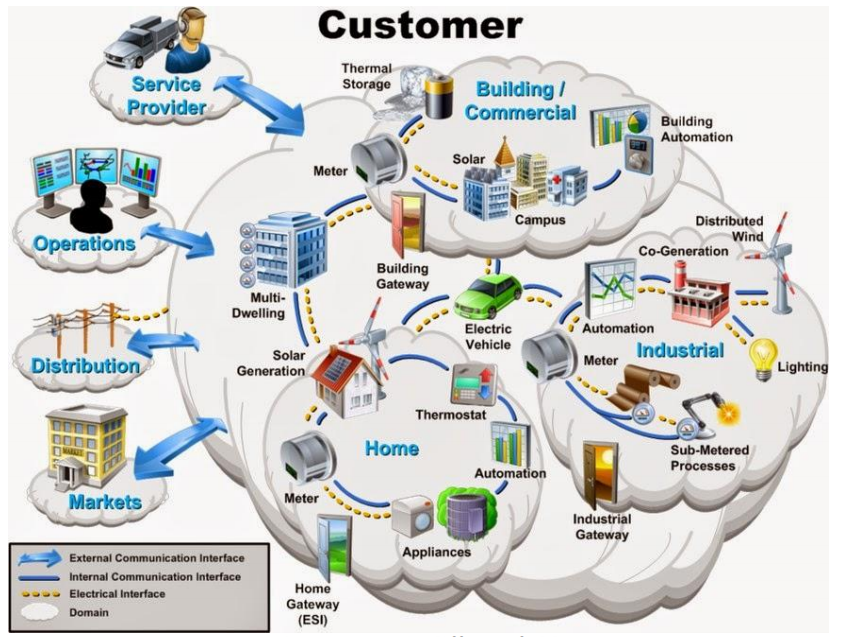
\includegraphics[height=8cm,width=12cm]{Figures/1.png}
	\caption{Το διαδίκτυο των αντικειμένων σε διάφορους τομείς \cite{Niranjan} }	
\end{figure}

%----------------------------------------------------------------------------------------
\section{Η κατάσταση μέχρι σήμερα}
Το διαδίκτυο των Αντικειμένων στη βιομηχανία βρίσκεται ακόμα σε πρώιμο στάδιο, παρόμοιο με αυτό που το διαδίκτυο βρισκόταν στα τέλη της δεκαετίας του 1990. Ενώ η εξέλιξη του διαδικτύου τις τελευταίες δύο δεκαετίες παρέχει κάποια σημαντικά διδάγματα, είναι αρκετά ασαφές το πως αυτή η γνώση μπορεί να αξιοποιηθεί στο Διαδίκτυο των Αντικειμένων στη βιομηχανία λόγω του μοναδικού πεδίου εφαρμογής του καθώς και λόγω των απαιτήσεων που υπάρχουν. Για παράδειγμα, οι αποκρίσεις σε πραγματικό χρόνο, είναι συχνά κρίσιμες στον κατασκευαστικό τομέα, στον τομέα της ενέργειας, της μεταφοράς καθώς και της υγείας. Ο πραγματικός χρόνος για το σημερινό Ίντερνετ συνήθως σημαίνει μερικά δευτερόλεπτα. Εν αντιθέσει, ο πραγματι­κός χρόνος σε ένα βιομηχανικό σύστημα είναι συχνά στην κλίμα­κα χιλιοστών του δευτερολέπτου Ο κανόνας του αντίχειρα (rule of thumb) υπαγορεύει ότι μία αλλαγή 10 φορές στην απόδοση απαι­τεί μία εντελώς διαφορετική προσέγγιση, για να μην αναφερθεί μια αλλαγή 100x  που θα επιφέρει στην βιομηχανία το Διαδίκτυο των Αντικειμένων [10].

Ένας άλλος σημαντικός παράγοντας πέρα από το χρόνο εί­ναι και η αξιοπιστία. Το ίντερνετ μέχρι στιγμής ακολουθεί μία προσέγγιση “καλύτερης προσπάθειας” (best-effort approach) η οποία παρέχει αποδεκτές επιδόσεις για τον άνθρωπο και για την αλληλεπίδραση του με το διαδίκτυο. Οι απροσδόκητες δυσλει­τουργίες σε έναν διακομιστή στην Google προκαλούν κάποιες κα­θυστερήσεις οι οποίες είναι αποδεκτές και δεν επηρεάζουν τόσο την αλληλεπίδραση του χρήστη με τις υπηρεσίες που του παρέχο­νται. Ωστόσο, η αποτυχία ενός ηλεκτρικού δικτύου, του συστήμα­τος ελέγχου της εναέριας κυκλοφορίας ή ενός αυτοματοποιημένου εργοστασίου για το ίδιο χρονικό διάστημα θα είχε πολύ πιο σοβα­ρές συνέπειες. 

Αυτοί οι παράγοντες της απόκρισης σε πραγματικό χρόνο και της αξιοπιστίας, που συνέβαλαν σε μία συντηρητική κουλτού­ρα μεταξύ των βιομηχανικών εταιρειών για την ενσωμάτωση των αλλαγών και των νέων τεχνολογιών, μαζί με το κόστος και την διάρκεια ζωής ενός τυπικού βιομηχανικού προϊόντος, είναι όλοι κρίσιμοι παράγοντες στη διαμόρφωση του τρόπου εξέλιξης του Διαδικτύου των Αντικειμένων στην Βιομηχανία.

Παρά τα εμπόδια αυτά, η υιοθέτηση του Διαδικτύου των Αντικειμένων στην βιομηχανία επιταχύνετε. Κατά τα τελευταία τρία χρόνια για παράδειγμα, ο αριθμός αισθητήρων που μεταφέρ­θηκαν αυξήθηκε περισσότερο από πέντε φορές. Πιο συγκεκρι­μένα, από 4,2 δισεκατομμύρια το 2012 αυξήθηκαν σε 23.6 δισεκα­τομμύρια το 2014 [11]. Μεγάλη προσοχή έχουν τραβήξει επίσης, οι προσπάθειες μεγάλων εταιρειών καθώς και κυβερνητικές πρω­τοβουλίες όπως το Industrie 4.0 [10].

Η Industry 4.0 είναι μία πολυετής στρατηγική πρωτοβουλία που πρόσφατα εισήγαγε η Γερμανική κυβέρνηση. Ο στόχος της πρωτοβουλίας αυτής είναι ο μετασχηματισμός της βιομηχανικής παραγωγής μέσω της ψηφιοποίησης και της εκμετάλλευσης των νέων δυνατοτήτων που προσφέρουν οι νέες τεχνολογίες. Η βιομη­χανική παραγωγή καθοδηγείται σήμερα από τον παγκόσμιο αντα­γωνισμό και την ανάγκη ταχείας προσαρμογής της παραγωγής στις συνεχώς μεταβαλλόμενες απαιτήσεις της αγοράς. Αυτές οι απαιτήσεις μπορούν να ικανοποιηθούν μόνο με ριζικές προόδους στην τρέχουσα τεχνολογία παραγωγής. Τα τεχνικά ζητήματα αυ­τών των απαιτήσεων αντιμετωπίζονται με την εφαρμογή των γε­νικών εννοιών των Cyber-Physical συστημάτων (CPS) και Διαδι­κτύου των Αντικειμένων στα συστήματα βιομηχανικής πα­ραγωγής [12].

Το Διαδίκτυο των Αντικειμένων στην βιομηχανία παρουσιάζεται σαν μία επανάσταση που υπόσχεται να αλλάξει ριζικά το πρόσωπο της βιομηχανίας. Στην πραγματικότητα, πρόκειται για μία εξέλιξη που έχει τις ρίζες της σε τεχνολογίες και λειτουργίες που έχουν αναπτυχθεί πριν από περισσότερα από 15 χρόνια. Η εμφάνιση του IIoT δημιούργησε τόσο ελπίδα όσο και σύγχυση σε φορείς που είναι υπεύθυνοι για την λειτουργία βιομηχανικών εγκαταστάσεων [13]. 

Ωστόσο, το Διαδίκτυο των Αντικειμένων στην βιομηχανία έχει να αντιμετωπίσει αρκετές προκλήσεις τόσο ερευνητικές όσο και τεχνολογικές. Οι πιο σημαντικές προκλήσεις που πρέπει να αντιμετωπιστούν σύμφωνα με την [14] είναι οι εξής:

\begin{enumerate}
	\item{\textbf{Τεχνολογική διαλειτουργικότητα}: Η διαλειτουργικότη­τα είναι σημαντικά πιο δύσκολη για το διαδίκτυο των αντικειμένων, καθώς δεν είναι μόνο η σύνδεση των ανθρώπων με τους ανθρώπους, αλλά η απρόσκοπτη αλληλεπίδραση μεταξύ συσκευών και ατόμων με συσκευές. Αυτές οι συσκευές μπορεί να διαφέρουν όσον αφορά τις τεχνολογικές τους δυνατότητες.}
	\item{\textbf{Σημασιολογική διαλειτουργικότητα}: Για να επιτευχθεί πλήρης διαλειτουργικότητα, είναι απαραίτητο οι συσκευές να ερμηνεύουν σωστά τις πληροφορίες κοινής χρήσης και να ενεργούν ανάλογα. Μία τέτοιου είδους διαλειτουργικότητα καλύπτεται από την σημασιολογι­κή πτυχή της διαλειτουργικότητας που συνήθως αναφέρεται σαν μοντέλο πληροφοριών (Information Model). Ως εκ τούτου, πρέπει να γίνουν βελτιώσεις όσον αφορά τις κατανεμημένες οντολογίες, τον σημα­σιολογικό ιστό (semantic web) καθώς και την ανακάλυ­ψη συσκευών μέσω σημασιολογίας. }
	\item{\textbf{Ασφάλεια και προστασία προσωπικών δεδομένων}: Η ακεραιότητα των δεδομένων, η μοναδική αναγνώριση καθώς και η κρυπτογράφηση θεωρούνται βασικές προκλήσεις για το Διαδίκτυο καθώς πολλά από τα δεδο­μένα που κοινοποιούνται περιέχουν προσωπικές πληροφορίες. Επιπλέον, τα δικαιώματα ιδιοκτησίας δεδο­μένων, τα νομικά ζητήματα και τα ζητήματα ευθύνης πρέπει να αντιμετωπιστούν αναλόγως. Τέλος, πρέπει να λαμβάνονται υπόψη οι ενεργειακά αποδοτικές τε­χνολογίες κρυπτογράφησης και προστασίας δεδομένων. }
	\item{\textbf{Έξυπνα αντικείμενα}: Πρέπει να αναπτυχθούν κυκλώμα­τα και συσκευές εξαιρετικά χαμηλής ισχύος ικανά να αντέχουν σε σκληρά περιβάλλοντα Επιπλέον, η παράλληλη επεξεργασία σε συστήματα πολλαπλών επεξεργαστών χαμηλής ισχύος, η προσαρμογή, η αυτόνομη συμπεριφορά με ταυτόχρονη εγγύηση της εμπιστοσύνης της ιδιωτικής ζωής και της ασφάλειας συγκαταλέγονται στις βασικές προκλήσεις όσον αφορά τις συσκευές του διαδικτύου. }
	\item{\textbf{Ανθεκτικότητα και αξιοπιστία}: Σε βιομηχανικά περιβάλλοντα ή σε περιπτώσεις έκτακτης ανάγκης, προσω­ρινές υπολειτουργίες του συστήματος δεν είναι αποδε­κτές. Ως εκ τούτου, τα ζητήματα ανθεκτικότητας και αξιοπιστίας στο διαδίκτυο πρέπει να διερευνηθούν από μια συνολική άποψη του συστήματος και επιπλέον πε­ριλαμβάνουν πτυχές όπως η διαθεσιμότητα, η ευρωστία και η ευελιξία της επικοινωνίας και του υλικού στις μεταβαλλόμενες περιβαλλοντικές συνθήκες, η αποφυγή ενιαίων σημείων αποτυχίας ή η ευρωστία δεδομένων επεξεργασίας σε αβέβαιες πληροφορίες. }
	
\end{enumerate}

Όταν αυτές οι προκλήσεις αντιμετωπιστούν, η διασύνδεση των βιομηχανικών συστημάτων παραγωγής με διάφορα άλλα συστήματα, συσκευές και καταναλωτές μέσω του διαδικτύου θα δημιουργήσει νέες δυνατότητες όπως αναφέρονται στο [15]: 

\begin{enumerate}
	\item{\textbf{Μαζική εξατομίκευση - Δημιουργία εξατομικευμένων προϊόντων με μικρούς χρόνους παράδοσης}: Πάντα υπήρχε ένας συμβιβασμός που έπρεπε να κάνει ένας κατασκευαστής μεταξύ εξατομίκευσης ενός προϊόντος και μαζικής παραγωγής του. Με την εφαρμογή του Δια­δικτύου των Αντικειμένων στην βιομηχανία ένα δι­κτυωμένο - έξυπνο εργοστάσιο καθιστά εφικτή την εξατομίκευση των προϊόντων σε κλίμακα μαζικής πα­ραγω-γής.}
	\item{\textbf{Συνεργασία ανθρώπου - μηχανής}: Η συνεργασία ανθρώπου - μηχανής μπορεί να διαχωριστεί σε φορητές διεπαφές ανθρώπου - μηχανής (mobile Hu­man-Machine Interfaces, HMI) και συνεργατικά συστήματα ανθρώπου - μηχανής (Human-Machine Collaborative Systems, HMCS). Οι HMI τεχνολογίες, για παράδειγμα κινητά τηλέφωνα, ταμπλέτες, ηλεκτρονικά που φοριούνται (wearables) σε συνδυασμό με πρόσβαση στο διαδίκτυο θα αλλάξουν ριζικά τον τρόπο με τον οποίο οι χειρι­στές των μηχανών και οι μηχανικοί θα παρακολουθούν και θα χειρίζονται την παραγωγή. Η φυσική παρουσία του προσωπικού στο χώρο διαχείρισης δεν θα είναι απαραίτητη, γεγονός που αυξάνει την ασφάλεια και οι ικανότητες του χειριστή διευρύνονται με την χρήση νέων τεχνολογιών όπως η εικονική πραγματικότητα για την καλύτερη παρακολούθηση της παραγωγής και τον εντοπισμό των προβλημάτων. Οι HMCS τεχνολογί­ες στοχεύουν στην κατασκευή ευέλικτων ρομποτικών συστημάτων για κατασκευαστές μικρής κλίμακας οι οποίοι τροποποιούν συχνά τις γραμμές παραγωγής τους. Η δυνατότητα ανάλυσης αλυσίδας ενεργειών (Action Sequence analysis) θα δίνει τη δυνατότητα στα ρομποτικά συστήματα αυτά να “μαθαίνουν” δυναμικά νέες εργασίες όπως η συναρμολόγηση κάποιου νέου προϊόντος με επαναληπτικές μεθόδους αντί για προ­γραμματισμό, πράγμα που μπορεί εύκολα να γίνει από ένα εργαζόμενο χωρίς αυτός να έχει ιδιαίτερες γνώσεις προγραμματισμού. }
	\item{\textbf{Ενοποίηση της παγκόσμιας αλυσίδας εφοδιασμού}: Η παγκοσμιοποίηση της αγοράς και των αλυσίδων εφοδιασμού, παρόλο που είναι εξαιρετικά κερδοφόρα για τον κατασκευαστή, δημιουργεί ορισμένα προβλήματα. Οι κατασκευαστές οφείλουν να λαμβάνουν υπ’ όψη τους πολλούς παράγοντες όπως οι τρέχουσες τιμές, διαθεσιμότητες, χρόνοι παράδοσης, ποιοτικές προδια­γραφές και αποθέματα πρώτων υλών, εργαλείων και μηχανών. Στα πλαίσια του Διαδικτύου των Αντικει­μένων στην βιομηχανία αναπτύσσονται εργαλεία τα οποία παρέχουν ενοποιημένη πρόσβαση σε πραγματικό χρόνο στις πληροφορίες αυτές. Κάτι τέτοιο ενισχύει την παραγωγικότητα, την ασφάλεια στο χώρο εργασίας και την ποιότητα της παραγωγής.}
\end{enumerate}

Η εφαρμογή της τεχνολογίας του Διαδικτύου των Αντικειμένων σε τομείς της βιομηχανίας αναμένεται να έχει έντονο αντίκτυπο σε όλη την διαδικασία της παραγωγής ώστε τελικά να οδηγήσει στην επονομαζόμενη τέταρτη βιομηχανική επανάσταση. Η εικόνα 2.2 δείχνει τις φάσεις που πέρασε η βιομηχανική επανάσταση.

\begin{figure}[htbp]
	\centering
		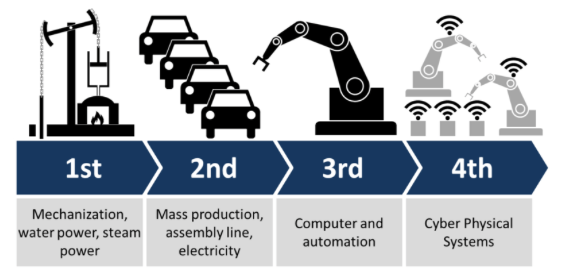
\includegraphics[height=7.5cm,width=15cm]{Figures/2.png}
	\caption{Οι φάσεις των βιομηχανικών επαναστάσεων \cite{Marr} }	
\end{figure}

Οι πιο αισιόδοξες προβλέψεις κάνουν λόγο για παραγωγή επιπρόσθετης αξίας παγκοσμίως από την εφαρμογή τους Διαδι­κτύου των Αντικειμένων στην βιομηχανίας της τάξης των 15 τρισεκατομμυρίων δολαρίων μέχρι το 2030 [16].  
%----------------------------------------------------------------------------------------
\section{Πρότυπα και πρωτόκολλα ΙοΤ}
Στο όραμα του Διαδικτύου των Αντικειμένων, το διαδίκτυο εξαπλώνεται πέρα από τον πυρήνα του. Αυτή η τεράστια ανάπτυ­ξη φέρνει τόσο συναρπαστικές δυνατότητες όσο και προκλήσεις στο Διαδίκτυο, όπως το πως θα ενσωματωθούν απρόσκοπτα οι διάφορες συσκευές και οι σένσορες στον παγκόσμιο ιστό. Ένας τρόπος για την ομαλή ενοποίηση του κυβερνο-κόσμου  και του φυσικού κόσμου είναι η επαναχρησιμοποίηση των υφιστάμενων τεχνολογιών και προτύπων στον παγκόσμιο ιστό, όσο το δυνατόν περισσότερο. Αυτή την τάση έρευνας την αντιμετωπίζει το Διαδί­κτυο των Αντικειμένων ως το Διαδίκτυο των πραγμάτων (Web of Things, WoT). Στο WoT, οι συσκευές δεν έχουν απλά μία ΙΡ ώστε να είναι συνδεδεμένες στο διαδίκτυο, αλλά έχουν την δυνατότητα να μιλούν και την ίδια γλώσσα και έτσι είναι σε θέση να επικοινω­νούν και να αλληλεπιδρούν ελεύθερα στον Παγκόσμιο Ιστό. Προ­κειμένου να υλοποιηθεί αυτό το όραμα, πρέπει να διεξαχθεί εκ νέου σχεδιασμός και βελτιώσεις στην κωδικοποίηση ωφέλιμου φορτίου και στα πρωτόκολλα εφαρμογής, ώστε να ικανοποιηθούν οι ειδικές απαιτήσεις των εφαρμογών μηχανής προς μηχανή (Machine to Machine, M2M) σε περιορισμένα περιβάλλοντα του διαδικτύου των αντικειμένων [17].

	Ένας τρόπος να εκπληρωθούν τα παραπάνω ζητούμενα είναι η ευρεία τοποθέτηση κοινής αρχιτεκτονικής, τόσο σε επίπεδο δικτύου, το οποίο επιτυγχάνεται με τα 6LoWPAN πρότυπα [19], όσο και σε επίπεδο εφαρμογών μέσω του WoT [20] που αναφέρθηκε παραπάνω. Μία τέτοια προσέγγιση επιτυγχάνει την χαλαρή ζεύξη (loose coupling) μεταξύ των τμημάτων που αποτελούν μια κατα­νεμημένη εφαρμογή, ιδιότητα - κλειδί για την επίτευξη της ζητού­μενης διαλειτουργικότητας [18]. 
	
\subsection{Η αρχιτεκτονική REST}
Η αρχιτεκτονική αρχή που βρίσκεται στην καρδιά του διαδικτύου, δηλαδή η Representatio-nal State Transfer (REST) όπως ορίστηκε από τον Roy Fielding [31], μοιράζεται έναν παρόμοιο στόχο με τις περισσότερες γνωστές τεχνικές ενοποίησης όπως οι υπηρεσίες WS-*  Web  services  (SOAP,  WSDL,  κτλ), ο οποίος εί­ναι η αύξηση της διαλειτουργικότητας για μια χαλαρότερη ζεύξη μεταξύ τμημάτων των κατανεμημένων εφαρμογών. Ωστόσο, ο στόχος του REST είναι να το επιτύχει αυτό με έναν πιο ελαφρύ και απλούστερο τρόπο και εστιάζει σε πόρους και όχι σε λειτουργίες, όπως συμβαίνει με τις υπηρεσίες WS-* Web. Συγκεκριμένα, το REST χρησιμοποιεί το Διαδίκτυο ως μια πλατφόρμα εφαρμογών και εκμεταλλεύεται πλήρως όλες τις λειτουργίες που είναι εγγε­νείς στο HTTP πρωτόκολλο, όπως ο έλεγχος ταυτότητας, η εξου­σιοδότηση, η κρυπτογράφηση, η συμπίεση και η προσωρινή απο­θήκευση. Με αυτόν τον τρόπο το REST “φέρνει” υπηρεσίες μέσα στον πρόγραμμα περιήγησης. Οι πόροι μπορούν να συνδεθούν και να ανατεθούν σε σελιδοδείκτες και τα αποτελέσματα να είναι ορατά με οποιοδήποτε πρόγραμμα περιήγησης του ιστού χωρίς να χρειάζεται να παράγουν πολύπλοκο πηγαίο κώδικα από αρχεία WSDL για να μπορούν να αλληλεπιδρούν με μία υπηρεσία [18]. 
	
	Για να το πετύχει αυτό η REST αρχιτεκτονική απαρτίζεται από δύο βασικούς κανόνες: 
	
\begin{itemize}
	\item{Το μοντέλο εφαρμογής μετασχηματίζεται και αντί να έχει την λειτουργικότητα σαν κύριο άξονα έχει τα δεδο­μένα. Αυτό σημαίνει ότι κάθε τι που προσφέρει υπηρε­σίες γίνεται πλέον ένας πόρος (resource), για παράδειγμα ένας αισθητήρας θερμότητας είναι ένας πόρος, που μπορεί να αναγνωριστεί μέσω ενός συγκεκριμένου URI.}
	\item{Οι τέσσερις κύριες λειτουργίες που παρέχονται από το πρωτόκολλο HTTP (PUT, POST, GET, DELETE) είναι οι μόνες διαθέσιμες λειτουργίες που μπορεί να έχει ένας πόρος. Έτσι ορίζεται μια ομοιόμορφη διεπαφή με γνωστή και κοινή σημασιολογία. }
\end{itemize}

 Αυτά τα πλεονεκτήματα εξηγούν κυρίως γιατί οι υπηρεσίες που προσφέρει η REST αρχιτεκτονική αποτελούν την τεχνολογική βάση για ένα αυξανόμενο αριθμό υπηρεσιών Web 2.0 όπως αυτές που προσφέρονται από το Flickr, το Twitter, το Google και το Amazon. Παραδοσιακά, η REST αρχιτεκτονική έχει χρησιμοποιη­θεί για την ενσωμάτωση διάφορων υπηρεσιών που παρέχονται σε ιστοσελίδες. Ωστόσο, επειδή η αρχιτεκτονική αυτή είναι αρκετά ελαφριά γίνεται άμεσα υποψήφια για ενσωματωμένες συσκευές με περιορισμένους πόρους ώστε να προσφέρουν υπηρεσίες στον παγκόσμιο ιστό. Εφόσον, τέτοιες συσκευές προσφέρουν συνήθως απλές και ατομικές λειτουργίες η μοντελοποίησή τους χρησιμοποιώντας το REST είναι συχνά απλή [18]. 

	Έχει σημασία να επισημανθεί πως το REST δεν περιγράφει κάποιο συγκεκριμένο πρωτόκολλο αλλά έχει μόνο ένα στυλ σχεδιασμού πρωτοκόλλων επικοινωνίας.

\subsection{Τα πρωτόκολλα HTTP - CoAP}
Επί του παρόντος, η πρόσβαση στο Διαδίκτυο απαιτεί πρωτόκολλα εφαρμογών μέσω TCP / IP  ή UDP / IP. Ένα τέτοιο πρωτόκολλο εφαρμογής αποτελεί το Hyper Text Transfer Protocol (HTTP), το οποίο έχει τυποποιηθεί στο ΙΕTF, και έχει εφαρμοστεί για την επικοινωνία στο διαδίκτυο. Ωστόσο, όταν εφαρμόζεται αυτό το πρωτόκολλο στην επικοινωνία μεταξύ συσκευών στο ΙοΤ, κατά την οποία μεταφέρεται ένας τεράστιος αριθμός μικροσκοπι­κών μπλοκ δεδομένων, το overhead που προστίθεται σε συνδυα­σμό με τις χαμηλές επιδόσεις αποτελούν ένα σημαντικό πρόβλη­μα. Επιπλέον, η διεύθυνση ΙΡ εξαρτάται από την φυσική τοποθε­σία της συσκευής, γεγονός που δημιουργεί το πρόβλημα της πολυπλοκότητας του ελέγχου δικτύου. 

	 Επιπλέον ένα μέρος της διαδρομής του δικτύου που θα ακολουθούν τα δεδομένα θα είναι μέσα σε δίκτυα χαμηλής ισχύος και με υψηλό ποσοστό απώλειας δεδομένων (Low power and Lossy Networks, LLN) [21]. Έτσι λοιπόν ένα κατάλληλο για την M2M επικοινωνία πρωτόκολλο πρέπει να μεγιστοποιεί την εξοικονόμηση ενέργειας, να είναι αποδοτικό όταν χρησιμοποιείται σε LLN’s και να είναι σχετικά ελαφρύ ώστε να εκτελείται σε μικρών δυνατοτή­των (μνήμης και επεξεργαστικής ισχύος) ενσωματωμένα συστή­ματα. Επιπρόσθετα το HTTP δε διαθέτει κάποιο μηχανισμό για αποστολή multi cast και εντοπισμού resources.

	Τα προβλήματα αυτά έρχεται να λύσει το πρωτόκολλο Constrained Application Protocol (CoAP). Το CoAP είναι ένα πρωτόκολλο σύγχρονης αίτησης / απόκρισης επιπέδου εφαρμογής που σχεδιάστηκε από την Internet Engineering Task Force (IETF) για να στοχεύσει σε συσκευές περιορισμένων πόρων. Σχεδιάστη­κε χρησιμοποιώντας ένα υποσύνολο των μεθόδων του πρωτοκόλ­λου HTTP που το καθιστούν διαλειτουργικό με το HTTP [23]. 

	Το  CoAP λειτουργεί πάνω από UDP έτσι ώστε να είναι όλη η υλοποίησή του ελαφριά. Χρησιμοποιεί τις εντολές του ΗΤΤΡ, GET, POST, PUT και DELETE για την παροχή αλληλεπιδράσεων προσανατολισμένων σε πόρους σε μια αρχιτεκτονική πελάτη - διακομιστή (client - server). Το CoAP είναι ένα πρωτόκολλο  αίτησης / απόκρισης που χρησιμοποιεί τόσο σύγχρονες όσο και ασύγχρονες απαντήσεις. Ο λόγος για το σχεδιασμό ενός πρωτοκόλλου επι­πέδου εφαρμογής που βασίζεται σε UDP για την διαχείριση των πόρων είναι η κατάργηση του overhead που προσθέτει το TCP και η μείωση των απαιτήσεων σχετικά με το εύρος ζώνης [24]. Χρησι­μοποιώντας το αναξιόπιστο UDP, το CoAP υλοποίησε τους δικούς του μηχανισμούς για την επίτευξη αξιοπιστίας. Δύο bit στην κε­φαλίδα κάθε πακέτου αναφέρουν τον τύπο του μηνύματος και το απαιτούμενο επίπεδο ποιότητας υπηρεσίας (QoS).  Υπάρχουν τέσ­σερις τύποι μηνυμάτων: 
	
\begin{enumerate}
	\item{\textbf{Επιβεβαιώσιμο}: Ένα μήνυμα αίτησης που απαιτεί επιβεβαίωση (ACK). Η απόκριση μπορεί να αποσταλεί είτε συγχρόνως (εντός του ACK) είτε εάν χρειάζεται περισσότερος υπολογιστικός χρόνος, μπορεί να σταλεί ασύγχρονα με ένα ξεχωριστό μήνυμα.}
	\item{\textbf{Μη επιβεβαιώσιμο}: Ένα μήνυμα που δεν απαιτεί επιβεβαίωση.}
	\item{\textbf{Αναγνώρισης}: Επιβεβαιώνει τη λήψη ενός επιβεβαίωσιμου μηνύματος.}
	\item{\textbf{Επαναφοράς (Reset)}: Επιβεβαιώνει την λήψη ενός μηνύματος που δεν είναι δυνατή η επεξεργασία του.}
\end{enumerate}

Υπάρχει επίσης ένας απλός μηχανισμός μετάδοσης Stop - and - Wait για επιβεβαιωμένα μηνύματα και ένα πεδίο κεφαλίδας 16 bit σε κάθε πακέτο CoAP ονομάζεται message ID, το οποίο εί­ναι μοναδικό και χρησιμοποιείται για την ανίχνευση διπλότυπων.  

	Παρόλο που το CoAP δημιουργήθηκε για τις επικοινωνίες ΙοΤ και Μ2Μ, δεν περιλαμβάνει ενσωματωμένα χαρακτηριστικά ασφαλείας. Το πρωτόκολλο που προτείνεται για διασφάλιση των συναλλαγών μέσω του CoAP είναι το Datagram Transport Layer Security (DTLS) [25].

	Η εικόνα 2.3 αναπαριστά την αρχιτεκτονική του πρωτοκόλλου CoAP: 
	
	
\begin{figure}[htbp]
	\centering
		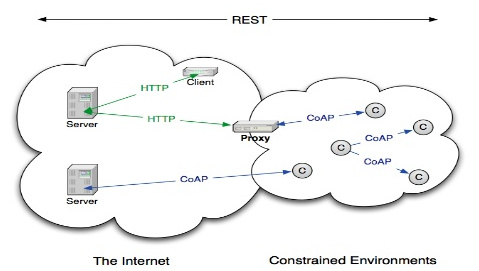
\includegraphics[height=8cm,width=12cm]{Figures/3.jpg}
	\caption{Η αρχιτεκτονική CoAP \cite{Coap} }	
\end{figure}

\subsection{Το πρωτόκολλο MQTT}
Το Message Queue Telemetry Transport (MQTT) πρωτόκολλο κυκλοφόρησε από την ΙΒΜ και στοχεύει σε ελαφρές επικοινωνίες μεταξύ συσκευών (Μ2Μ). Πρόκειται για ένα ασύγχρονο πρωτόκολλο δημοσίευσης / εγγραφής (publish / subscribe) που εκτελείται στην κορυφή του TCP.  Τα πρωτόκολλα δημοσίευσης / εγγραφής πληρούν καλύτερα τις απαιτήσεις του IoT από τα πρωτόκολλα αιτήματος / απόκρισης (request /response), δεδομένου ότι οι clients δεν χρειάζεται να ζητούν ενημερώσεις και έτσι το εύρος ζώνης του δικτύου μειώνεται και η ανάγκη χρήσης υπολογιστικών πόρων μειώνεται. 

Στο MQTT υπάρχει ένας broker (διακομιστής) που περιέχει ζητήματα. Κάθε πελάτης (client) μπορεί να είναι ένας εκδότης (publisher) που στέλνει πληροφορίες στον broker σχετικά με ένα συγκεκριμένο ζήτημα ή / και έναν συνδρομητή (subscriber) που λαμβάνει αυτόματα μηνύματα κάθε φορά που υφίσταται μία αλλαγή σε ένα ζήτημα στο οποίο έχει εγγραφεί. Το συγκεκριμένο πρωτόκολλο έχει σχεδιαστεί για να χρησιμοποιεί το εύρος ζώνης και τη χρήση μπαταρίας με φειδώ γι’ αυτό για παράδειγμα αυτή τη στιγμή χρησιμοποιείται από το Facebook Messenger [26]. 

Το ΜQTT εξασφαλίζει αξιοπιστία παρέχοντας την επιλογή τριών επιπέδων QoS: 
\begin{enumerate}
	\item{\textbf{Fire and forget}: Ένα μήνυμα αποστέλλεται μία φορά και δεν απαιτείται επιβεβαίωση.}
	\item{\textbf{Delivered at least one}: Ένα μήνυμα αποστέλλεται τουλάχιστον μία φορά και απαιτείται επιβεβαίωση.}
	\item{\textbf{Delivered exactly one}: Ένας μηχανισμός χειραψίας τεσσάρων κατευθύνσεων χρησιμοποιείται για να εξασφαλίσει ότι το μήνυμα παραδίδεται ακριβώς μία φορά. }
\end{enumerate}

Aξίζει να σημειωθεί ότι παρόλο που το MQTT τρέχει πάνω από το TCP, έχει σχεδιαστεί ώστε να προσθέτει χαμηλό overhead σε σύγκριση με άλλες εφαρμογές που βασίζονται στο TCP [27]. Η εικόνα 2.4 δείχνει την αρχιτεκτονική του MQTT  πρωτοκόλλου.


\begin{figure}[htbp]
	\centering
		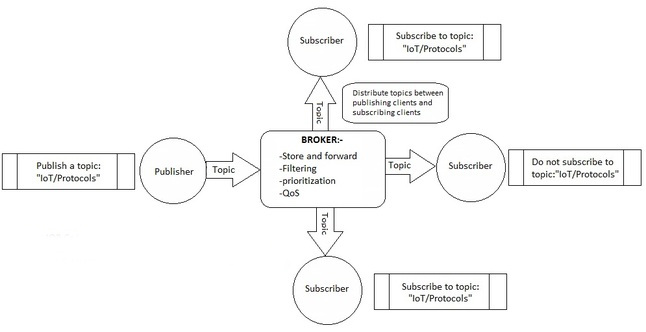
\includegraphics[height=8cm,width=15cm]{Figures/4.jpg}
	\caption{Η αρχιτεκτονική MQTT \cite{Gupta} }	
\end{figure}

Ενδεικτικά, άλλα διαδεδομένα πρωτόκολλα είναι τα XMPP, DDS, SOAP και WebSocket.


\chapter{Το πρωτόκολλο LwM2M } % Main chapter title

\label{Chapter3} 

%\lhead{ΤΟ ΠΡΩΤΟΚΟΛΛΟ LWM2M} 

%%%%%%%%%%%%%%%%%%%%%%%%%%%% The paper headers

\section{Γενικά}
Το Lightweight M2M (\textbf{LwM2M}) αποτελεί ένα νέο, αναδυόμενο πρότυπο που αναπτύχθηκε από την Open Mobile Alliance (OMA) με μεγάλη συνάφεια με την αναπτυσσόμενη M2M βιομηχανία και το Διαδίκτυο των Αντικειμένων στο σύνολο του. Αυτό το βιομηχανικό πρότυπο παρέχει μέσα για την απομακρυσμένη διαχείριση μιας ευρείας γκάμας απομακρυσμένων ενσωματωμένων συσκευών και συνδεδεμένων συσκευών στο αναδυόμενο Διαδίκτυο των Αντικειμένων για την πραγματοποίηση εξ’ αποστάσεως εξυπηρέτησης και διαχείρισης απομακρυσμένων εφαρμογών [28].  

Η αγορά των διασυνδεδεμένων συσκευών αυξάνεται ρα­γδαία. Παρόλο που υπάρχουν βιομηχανικά πρότυπα διαθέσιμα που ικανοποιούν τις απαιτήσεις απομακρυσμένης διαχείρισης, για παράδειγμα σταθερών ευρυζωνικών δρομολογητών και smartphones, αυτά τα καθιερωμένα πρότυπα δεν είναι ιδιαίτερα χρήσιμα για την απομακρυσμένη διαχείριση μιας μεγάλης και ανα­πτυσσόμενης κατηγορίας συνδεδεμένων συσκευών: εκείνων με περιορισμένο εύρος ζώνης δικτύου, υπολογιστικής ισχύος και μνήμης, εκείνων που εξαρτώνται από περιορισμένη διάρκεια ζωής της μπαταρίας και εκείνων που είναι βιώσιμα μόνο με πολύ χαμη­λό κόστος παραγωγής. Ως εκ τούτου, αναλήφθηκε αυτή η νέα προ­σπάθεια για τη δημιουργία ενός μηχανισμού που να καλύπτει επίσης τις ανάγκες των “περιορισμένων” συσκευών. Η βιομηχα­νία αναζητά έναν απλό, χαμηλού κόστους απομακρυσμένο μηχανι­σμό διαχείρισης και ενεργοποίησης υπηρεσιών, ο οποίος να περιλαμβάνει σύγχρονες αρχιτεκτονικές αρχές (σύμφωνα με τα πρότυ­πα του Διαδικτύου) ενώ παράλληλα να λειτουργεί μέσω ασύρμα­των συνδέσεων και να είναι κατάλληλος για το σκοπό αυτό λόγω των χαμηλών απαιτήσεων σε πόρους. Τη λύση έρχεται να δώσει το πρωτόκολλο LwM2M.

Από τεχνικής άποψης, το LwM2M πρόκειται για ένα πρωτόκολλο επικοινωνίας για χρήση μεταξύ του λογισμικού του client μιας M2M συσκευής και του λογισμικού του server σε μια πλατφόρμα διαχείρισης και ενεργοποίησης υπηρεσιών Μ2Μ. Το πρωτόκολλο LwM2M που χρησιμοποιείται για την απομακρυσμένη διαχείριση Μ2Μ συσκευών και τις σχετικές δυνατότητες εξυπηρέτησης έχει τέσσερα εξαιρετικά χαρακτηριστικά [28]:

\begin{enumerate}
	\item{Διαθέτει σύγχρονο αρχιτεκτονικό σχεδιασμό βασι­σμένο στο REST που απευθύνεται σε προγραμματιστές.}
	\item{Ορίζει ένα μοντέλο πόρων και δεδομένων.}
	\item{Έχει σχεδιαστεί με γνώμονα την απόδοση και τους περιορισμένους πόρους των συσκευών Μ2Μ.}
	\item{Επαναχρησιμοποιείται και βασίζεται σε ένα αποδοτικό πρότυπο μεταφοράς δεδομένων, το CoAP που περιγράφηκε παραπάνω.}
\end{enumerate}

Η διαθεσιμότητα αυτού του ανοικτού κώδικα, τυποποιη­μένου μηχανισμού απομακρυσμένης διαχείρισης δημιουργεί τις ακόλουθες ευκαιρίες και επιχειρηματικά οφέλη για τους διάφο­ρους “παίκτες” της βιομηχανίας Μ2Μ [28]:

\begin{itemize}
	\item{Θα μειώσει τον βαθμό κατακερματισμού (fragmentation) στον τομέα της απομακρυσμένης διαχείρισης συσκευών M2Μ, επιτρέποντας έτσι περισσότερες plug-n-play λύσεις μεταξύ μιας αυξανόμενης ποικιλίας συσκευών Μ2Μ και των πλατφορμών διαχείρισης τους.}
	\item{Δεδομένου του σχεδιασμού του για την κάλυψη των περιορισμένων συσκευών, μπορεί να λειτουργήσει ως ένας παράγοντας που διευκολύνει την ανάπτυξη της αγοράς Μ2Μ σε διάφορους τομείς, από την διαχείριση μίας “έξυπνης” πόλης μέχρι την διαχείριση ενέργειας και την παρακολούθηση θέσης. Πιο συγκεκριμένα θα ωφεληθούν τομείς όπου οι συσκευές πρέπει να έχουν χαμηλό κόστος για να καταστήσουν δυνατή την ανάπτυξη βιώσιμων επιχειρηματικών μοντέλων.}
	\item{Αυτό το νέο πρότυπο θα μπορούσε να βελτιώσει σημαντικά τον χρόνο time-to-market και την διαχειρισιμότητα των συσκευών, παρέχοντας για  πρώτη φορά μια λύση που μπορεί να χρησιμοποιηθεί τόσο για την διαχείριση συσκευών όσο και για εφαρμογές δεδομένων και υπηρεσιών, ανεξάρτητα από το πως φιλοξενούνται τα στοιχεία του συστήματος.}
	\item{Ως πρωτόκολλο απομακρυσμένης διαχείρισης μεταξύ συσκευών και πλατφορμών Μ2Μ οδηγεί σε αποσύνδεση και των δύο πλευρών, επιτρέποντας έτσι μεγαλύτερη ανεξάρτητη καινοτομία των συσκευών Μ2Μ και των πλατφορμών Μ2Μ. }
\end{itemize}

\section{Περιγραφή των μηχανισμών του LwM2M}
Το LwM2M είναι βασισμένο και σχεδιασμένο πάνω στο CoAP και χρησιμοποιεί προαιρετικά το πρωτόκολλο DTLS για την ανάπτυξη εφαρμογών που απαιτούν ασφαλή επικοινωνία. Στην ει­κόνα 3.1 δίνεται μία οπτικοποίηση της αρχιτεκτονικής του LwM2M πρωτοκόλλου. Μια προς διαχείριση συσκευή αποτελεί έναν LwM2M client ενώ η πλατφόρμα διαχείρισης της συσκευής είναι ένας LwM2M server. Για την επικοινωνία μεταξύ αυτών των δύο το LwM2M ορίζει τέσσερα interfaces που είναι τα εξής:

\begin{enumerate}
	\item{\textbf{Bootstrap}: ορίζει την διαδικασία που απαιτείται ώστε ένας LwM2M client να λάβει τις απαιτούμενες πληροφορίες για τον server στον οποίο πρέπει να συνδεθεί (register).}
	\item{\textbf{Client Registration}: ορίζει την απαιτούμενη διαδικασία κατά την οποία ένας client εγγράφεται ή απεγγράφεται από έναν LwM2M server.}
	\item{\textbf{Device Management and Service Enablement}:  περιγράφει τον τρόπο με τον οποίο ένας LwM2M server προσπελαύνει τα LwM2M objects και τα LwM2M resources που έχει ένας LwM2M client.}
	\item{\textbf{Information Reporting}: χρησιμοποιείται από τον server για την παρακολούθηση αλλαγών σε κάποιο resource του client.}
\end{enumerate}

Ο client αλληλεπιδρά με τον server ακολουθώντας τις αρχές της REST αρχιτεκτονικής. Κάθε υπηρεσία ή πληροφορία που διαθέτει ένας LwM2M client στο περιβάλλον του αποτελεί ένα LwM2M resource. Κάθε resource μεταξύ των υπόλοιπων ιδιοτήτων του, χαρακτηρίζεται και από έναν τύπο (type). Ένα resource μπορεί να είναι τύπου {String, Float, Integer, Boolean, Opaque, Time, ObjLink}. Τα resources είναι λογικά ομαδοποιημένα σε LwM2M Objects. Ένας LwM2M client μπορεί να έχει οποιοδήποτε αριθμό από resources τα οποία όμως ανήκουν σε κάποιο object. Κάθε object μπορεί να έχει ένα μοναδικό ή πολλαπλά στιγμιότυπα (object instances).


\begin{figure}[htbp]
	\centering
		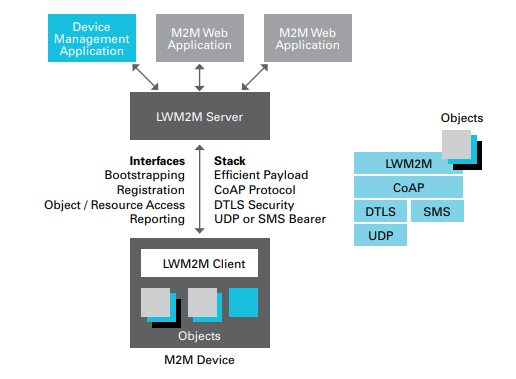
\includegraphics[height=10cm,width=15cm]{Figures/5.png}
	\caption{Η LwM2M αρχιτεκτονική \cite{OMA1} }	
\end{figure}

Κάθε {object/ object instance /resource ενός συγκεκριμένου object} αναγνωρίζεται μονοσήμαντα από ένα μοναδικό {object id/ object instance id / resource id} αντίστοιχα. Η αναφορά σε κάποιο resource γίνεται μέσα από ένα path με τη μορφή “/{Object ID}/{Object Instance ID}/{Resource ID}”. 
	
Ο LwM2M server όταν θέλει να ξεκινήσει μία αλληλεπίδραση με έναν LwM2M client του αποστέλλει ένα αίτημα. Ένα τέτοιο αίτημα απαρτίζεται από το path του resource στο οποίο αναφέρεται και την μέθοδο την οποία αιτείται να εφαρμοστεί στο resource αυτό. 	Το Device Management \& Service Enablement Interface (DM\&SE) ορίζει το σύνολο των μεθόδων που \textbf{πρέπει} να υποστηρίζει τόσο ένας LwM2M client όσο και ο LwM2M server και μπορούν να εφαρμοστούν σε ένα resource [32]. Αυτές είναι:
	
\begin{enumerate}
	\item{\textbf{CREATE}: Δημιουργεί instance}
	\item{\textbf{READ}: Ζητείται να επιστραφεί η τιμή ενός resource}
	\item{\textbf{WRITE}: Ζητείται η αλλαγή της τιμής ενός resource}
	\item{\textbf{DELETE}: Διαγραφεί instance}
	\item{\textbf{EXECUTE}: Ζητείται η πραγματοποίηση μίας ενέργειας}
	\item{\textbf{WRITE-ATTRIBUTES}: Χρησιμοποιείται για την αλλαγή των τιμών των attributes}
	\item{\textbf{DISCOVER}: Χρησιμοποιείται για την ανακάλυψη resources και attributes}
\end{enumerate}

Αφού ο LwM2M server αποστείλει το αίτημα ο LwM2M client στέλνει πίσω μία απάντηση η οποία περιέχει έναν κωδικό απάντησης και σε κάποιες περιπτώσεις ένα περιεχόμενο. Για παράδειγμα μια απάντηση σε ένα αίτημα READ μπορεί να έχει για κωδικό απάντησης το “2.04 Changed” και για περιεχόμενο την τιμή του resource το οποίο αφορούσε το αίτημα. Ανάλογα τον τύπο του αρχικού αιτήματος, ο κωδικός απάντησης έχει διαφορετική σημασία [32].	

	Μεγάλη σημασία έχει επίσης και ο μηχανισμός observe του CoAP, ο οποίος χρησιμοποιείται από το LwM2M μέσω του Information Reporting Interface. Αυτό το interface χρησιμοποιείται από έναν LwM2M server ώστε να παρατηρούνται οι αλλαγές που γίνονται σε ένα resource ενός καταχωρημένου LwM2M client. Κάθε φορά που αλλάζει η τιμή του resource αποστέλλεται μία ειδοποίηση στον LwM2M server μαζί με τη νέα τιμή του resource. Αυτή η σχέση observe-notify ξεκινά με την αποστολή ενός αιτήματος τύπου “observe”  από τον server στον client για ένα object, object instance ή resource που είναι παρακολουθήσιμο (observable).Μετά από την επιτυχή εγκαθίδρυση μιας τέτοιας σχέσης, ο LwM2M client αποστέλλει ένα μήνυμα τύπου “notify” στον server. Το μήνυμα αυτό περιέχει τη νέα τιμή του resource που παρακολουθείται. Η εικόνα 3.2 δείχνει το μοντέλο λειτουργίας για το συγκεκριμένο interface:

\begin{figure}[htbp]
	\centering
		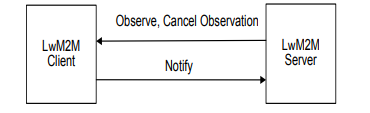
\includegraphics[height=3cm,width=9cm]{Figures/6.png}
	\caption{LwM2M Information Reporting Interface \cite{OMA2} }	
\end{figure}

Αξίζει να σημειωθεί ότι ο οργανισμός ΟΜΑ μαζί με τις προδιαγραφές του LwM2M δημοσιοποιεί και ένα μητρώο (registry) το οποίο περιέχει όλα τα LwM2M objects τα οποία έχουν καταχωρηθεί σε αυτό από τον οργανισμό καθώς και από τρίτους. Αυτό το μητρώο υλοποιήθηκε με στόχο ένας LwM2M client να μπορεί να ενημερώσει έναν LwM2M server για τα objects τα οποία μπορεί να υποστηρίξει αποστέλλοντας μόνο το object ID. Έτσι όλα τα χαρακτηριστικά καθώς και τα resources που αφορούν τα objects αυτά μπορούν να ανασυρθούν από αυτό το μητρώο που μπορεί να βρίσκεται είτε τοπικά στην μνήμη του LwM2M server είτε στο Διαδίκτυο. Επιπρόσθετα έχει υλοποιηθεί και άλλο ένα μητρώο το Resource Registry το οποίο περιέχει επαναχρησιμοποιούμενα resources τα οποία έχουν κοινά χαρακτηριστικά και σημασία για κάθε LwM2M object που τα χρησιμοποιεί. Στην συγκεκριμένη εργασία δημιουργήθηκε ένα μητρώο που βρίσκεται τοπικά στην μνήμη του LwM2M server.

	Επειδή η παρούσα εργασία αφορά την υλοποίηση του Industrial Automation Thing δεν δόθηκε ιδιαίτερη έμφαση στην υλοποίηση του LwM2M server. Εν αντιθέσει υλοποιήθηκε ο LwM2M client ώστε να χρησιμοποιηθούν τα πλεονεκτήματα που δίνονται από το LwM2M. Ο LwM2M server που χρησιμοποιήθηκε υλοποιήθηκε σε άλλη διπλωματική εργασία που εκπονήθηκε ταυτόχρονα με την παρούσα. 
	
\section{Πλεονεκτήματα του  LwM2M}

Το πρωτόκολλο LwM2M επιλύει ένα σύνολο τεχνολογικών προκλήσεων που σχετίζονται με την διαχείριση συσκευών και την ενεργοποίηση end-to-end υπηρεσιών καθώς η αγορά M2M ωριμάζει και το Διαδίκτυο των Αντικειμένων καθιστούν εφικτή την επικοινωνία μεταξύ τέτοιων συσκευών. Παρακάτω συνοψίζονται τα οφέλη που παρέχει το LwM2M [28]: 

\begin{itemize}
	\item{Μεγαλύτερη ανάπτυξη της αγοράς και αποδοτικότητα κόστους για ολόκληρη την βιομηχανία,  μέσω των τεχνολογιών που προσφέρει το LwM2M οι οποίες καθιστούν εφικτή την χαλαρή σύνδεση συσκευών, την εύκολη διαχείριση τους και την διαχείριση των υπηρεσιών που αυτές προσφέρουν.}
	\item{Οι πάροχοι υπηρεσιών, οι OEMs και οι τελικοί χρήστες επωφελούνται από την ομοιόμορφη διαχείριση των διάφορων συσκευών.}
	\item{Σε σύγκριση με τις protocol stacks που χρησιμοποιούνται στις παραδοσιακές συσκευές, το LwM2M μπορεί να παρέχει 10x αύξηση της αποδοτικότητας.}
	\item{Το LwM2M συμπληρώνει τις υπάρχουσες λύσεις διαχείρισης συσκευών, όπως το ΟΜΑ DM και το Broadband Forum TR-69, και επεκτείνει σε μεγάλο βαθμό το εύρος των συσκευών που μπορούν να διαχειριστούν με ασφάλεια.}
	\item{Το μοντέλο δεδομένων του LwM2M καθώς και το μητρώο των αντικειμένων παρέχουν προσβάσιμη και επαναχρησιμοποιήσιμη σημασιολογία τόσο για την διαχείριση συσκευών όσο και για την διαχείριση των δεδομένων μιας εφαρμογής για όλο το Διαδίκτυο των Αντικειμένων στην βιομηχανία. }
	\item{Παρέχοντας μια ενιαία λύση για την διαχείριση των συσκευών και των δεδομένων τους το LwM2M απλοποιεί τα διάφορα συστήματα και επιτρέπει την δημιουργία νέων και καινοτόμων υπηρεσιών M2M.}
	\item{Η πλήρης διαχείριση του κύκλου ζωής και της ασφάλειας που είναι κατάλληλη για περιορισμένες συσκευές επιλύει ένα από τα πιο πιεστικά προβλήματα στη βιομηχανία M2M.}
	\item{Το LwM2M ορίζει μόνο της διεπαφή δικτύου της συσκευής, επιτρέποντας έτσι την εύκολη ενσωμάτωση του σε υπάρχουσες υπηρεσίες διαχείρισης συσκευών και υπηρεσιών Μ2Μ.}
\end{itemize}





\addtocontents{toc}{\vspace{2em}}
\chapter{Ανάπτυξη λογισμικού με την προσέγγιση συνιστωσών } % Main chapter title

\label{Chapter4} 

\section{Εισαγωγή}
Για την μείωση της πολυπλοκότητας των συστημάτων λογισμικού, οι μηχανικοί λογισμικού έχουν εφεύρει αρκετές τεχνικές που στοχεύουν στην βελτίωση της επαναχρησιμοποίησης και της συντηρησιμότητας του λογισμικού όπως η μοντελοποίηση λογισμικού σε μονάδες (modules) και η αντικειμενοστρέφεια. Στην [33], αναφέρεται ότι το 53\% των συστημάτων λογισμικού δεν πέτυχε να παραδοθεί εντός του χρονοδιαγράμματος και του προϋπολογισμού, καθώς και με την απαιτούμενη λειτουργικότητα και ποιότητα, ενώ το 18\% των έργων εγκαταλείφθηκε πλήρως. Αυτά τα στοιχεία καθιστούν σαφή τη σημασία της ακριβής πρόβλεψης της προσπάθειας που απαιτείται για να αναπτυχθεί ένα νέο σύστημα λογισμικού. 

	Τα τελευταία χρόνια, μία δημοφιλής προσέγγιση ανάπτυξης λογισμικού, η ανάπτυξη λογισμικού βασισμένη σε components (Component Based Software Development, CBSD) έχει αλλάξει σημαντικά την κατάσταση που έχουν να αντιμετωπίσουν οι μηχανικοί λογισμικού. Στην βιομηχανία έχουν αναφερθεί σημαντικά πλεονεκτήματα που δίνει η χρήση της CBSD προσέγγισης ανάπτυξης λογισμικού έναντι του παραδοσιακού τρόπου ανάπτυξης λογισμικού [33]. Μετά την επιτυχία που είχε η Αντικειμενοστραφής προσέγγιση, η CBSD εμφανίζεται ως η επόμενη επανάσταση στον τρόπο ανάπτυξης λογισμικού [34]. Επιπλέον σύμφωνα με την [33] που αφορά τους τρόπους ανάπτυξης λογισμικού που εφαρμόζονται στην βιομηχανία, διαπιστώθηκε ότι περίπου το 53\% από 118 εταιρείες που συμμετείχαν σε έρευνα χρησιμοποιούν την CBSD και η τάση αυτή συνεχώς αυξάνεται. 
	
\section{Η προσέγγιση των συνιστωσών}

\subsection{Γενικές πληροφορίες και βασικές έννοιες}

Η ανάπτυξη λογισμικού με βάση τα components αποτελεί μία προσέγγιση βασισμένη στην επαναχρησιμοποίηση για τον ορισμό, την υλοποίηση και την σύνθεση χαλαρά συνδεδεμένων (loosely coupled) ανεξάρτητων components σε συστήματα λογισμικού. Επιδιώκει να επιφέρει ευρύ φάσμα πλεονεκτημάτων τόσο βραχυπρόθεσμα όσο και μακροπρόθεσμα για το ίδιο το λογισμικό και για οργανισμούς που χορηγούν τέτοιες λύσεις. Το σκεπτικό πίσω από αυτή την προσέγγιση είναι η συναρμολόγηση συστημάτων λογισμικού, χρησιμοποιώντας υπάρχοντα, κατασκευασμένα από τρίτους και δοκιμασμένα components έτσι ώστε να μην είναι απαραίτητη η υλοποίηση όλου του συστήματος από την αρχή. Ο κύκλος ζωής της CBSD μπορεί να χωριστεί σε τέσσερις φάσεις: \textbf{Domain analysis, Component Design and Development, Component Cataloging and Retrieval, Component Selection and Application Assembly} [35]. Κατά την ανάπτυξη ενός προϊόντος λογισμικού χρησιμοποιώντας την CBSD τεχνική, τα διαθέσιμα components συναρμολογούνται ή προσαρμόζονται με τη βοήθεια μίας εφαρμογής ανάπτυξης λογισμικού [34]. Στην εικόνα 4.1 δίνεται μία απεικόνιση της διαδικασίας που ακολουθείται κατά την ανάπτυξη ενός συστήματος λογισμικού χρησιμοποιώντας την CBSD προσέγγιση. 


\begin{figure}[htbp]
	\centering
		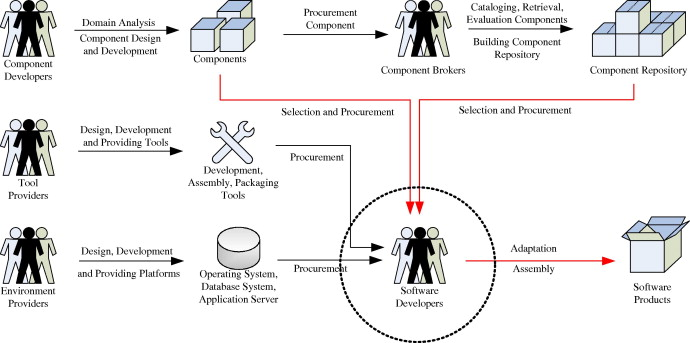
\includegraphics[height=8cm,width=15cm]{Figures/7.jpg}
	\caption{Διάγραμμα ροής της διαδικασίας CBSD \cite{Xie} }	
\end{figure}

\subsection{Οντότητες Λογισμικού}
\subsubsection{Component}
Σύμφωνα με το [36], οι χαρακτηριστικές ιδιότητες ενός component είναι:
\begin{enumerate}
	\item{Αποτελεί μία μονάδα που αναπτύσσεται ανεξάρτητα}
	\item{Μπορεί να αναπτυχθεί και από τρίτους}
	\item{Δεν έχει (εξωτερικά) παρατηρήσιμη κατάσταση}
\end{enumerate}

	Αυτές οι ιδιότητες έχουν πολλές συνέπειες. Για να μπορεί ένα component να αναπτύσσεται ανεξάρτητα, είναι απαραίτητο να διαχωρίζεται από το περιβάλλον στο οποίο θα χρησιμοποιηθεί και από τα άλλα components. Επομένως, ένα component ενθυλακώνει όλα τα χαρακτηριστικά του. Επίσης, καθώς αποτελεί μία μονάδα ανάπτυξης ενός συστήματος δεν θα χρησιμοποιηθεί ποτέ μόνο του. Σε αυτό το πλαίσιο γίνεται σαφές ότι μία ομάδα τρίτων που αναπτύσσει ένα component δεν είναι απαραίτητο να έχει πρόσβαση σε λεπτομέρειες κατασκευής ενός συστήματος καθώς ούτε και σε όλα τα υπόλοιπα components που απαρτίζουν το σύστημα [36]. 
	
	Για να μπορεί ένα component να συνδυαστεί με άλλα components που μπορεί να έχουν σχεδιαστεί και υλοποιηθεί από τρίτους πρέπει να είναι επαρκώς αυτόνομο [36]. Ένα component παρέχει ένα σύνολο υπηρεσιών (services) και τις εκθέτει στο περιβάλλον του μέσω ενός interface που ονομάζεται “provided interface”. Το component επίσης μπορεί να χρειαστεί κάποιες υπηρεσίες από άλλα components ή από το περιβάλλον στο οποίο λειτουργεί προκειμένου να παρέχει με επιτυχία τις δικές του . Αυτές οι απαιτούμενες υπηρεσίες συγκεντρώνονται στο “required interface” του component. Για το λόγο αυτό σε ένα σύστημα που αποτελείται από components κάθε component συναρμολογείται σε συνεργασία με άλλα components ώστε να μπορούν να καλυφθούν οι απαιτήσεις του. Το component ουσιαστικά ορίζει ένα είδος συμβατικής συμφωνίας με την οποία, αν ικανοποιηθούν όλες οι λειτουργικές ανάγκες της (απαιτούμενες υπηρεσίες), καθώς και άλλες πιθανές υποθέσεις για το περιβάλλον ή την πλατφόρμα εκτέλεσης, τότε είναι σε θέση να παρέχει τις λειτουργικές της υπηρεσίες [37]. Με άλλα λόγια, ένα component πρέπει να “κρύβει” την υλοποίηση του από το περιβάλλον του και να αλληλεπιδρά με αυτό μέσω καλά καθορισμένων interfaces [36].

	Τέλος, ένα component δεν πρέπει να έχει οποιαδήποτε εξωτερικά παρατηρήσιμη κατάσταση. Δηλαδή απαιτείται το component να μην διακρίνεται από τα δικά του αντίγραφα. Πιθανές εξαιρέσεις σε αυτό τον κανόνα είναι χαρακτηριστικά που δεν συμβάλουν στην λειτουργικότητα του component, όπως για παράδειγμα οι σειριακοί αριθμοί που χρησιμοποιούνται στην λογιστική. Ο συγκεκριμένος αποκλεισμός της παρατηρήσιμης κατάστασης επιτρέπει τεχνικές χρήσεις της κατάστασης που μπορεί να είναι κρίσιμες για την απόδοση χωρίς να επηρεάζεται η παρατηρήσιμη συμπεριφορά ενός component. Συγκεκριμένα, ένα component μπορεί να χρησιμοποιήσει μια κατάσταση για σκοπούς προσωρινής αποθήκευσης, π.χ. μια μνήμη cache [36].
	
\subsubsection{Interface}

	Τα interfaces αποτελούν σημαντικό στοιχείο των components. Το interface ενός component καθορίζει τις υπηρεσίες που αυτό παρέχει στο περιβάλλον του καθώς και τα σημεία πρόσβασης (access points) του. Κανονικά, ένα component θα απαρτίζεται από πολλά interfaces που θα αντιστοιχούν σε διαφορετικά σημεία πρόσβασης. Κάθε σημείο πρόσβασης μπορεί να παρέχει διαφορετική υπηρεσία, καλύπτοντας διαφορετικές ανάγκες. Ιδιαίτερη έμφαση πρέπει να δοθεί στον συμβατικό χαρακτήρα των προδιαγραφών ενός interface, καθώς το component και τα components που θα το χρησιμοποιήσουν αναπτύσσονται σε αμοιβαία άγνοια, οπότε η σύμβαση (contract) αυτή αποτελεί το κοινό μέσο για την επιτυχή αλληλεπίδραση των components [36]. Η εικόνα 8 δείχνει δύο components με τα interfaces τους.
	
\subsubsection{Container}

	Ο container μπορεί να θεωρηθεί σαν ένας software wrapper γύρω από τα components, ο οποίος είναι υπεύθυνος για την ικανοποίηση των έξω-λειτουργικών απαιτήσεων που τίθενται επί του component. Γενικά, δεν μπορεί να υπάρξει άμεση επικοινωνία μεταξύ των components. Αυτό εν μέρει προκαλείται από τον container μέσα στον οποίο βρίσκεται το component, ο οποίος είναι υπεύθυνος για την απόκτηση και έκθεση των απαιτούμενων και παρεχόμενων interfaces αντίστοιχα. Ο container επίσης, διαμεσολαβεί την πρόσβαση του component σε υπηρεσίες που παρέχονται από την πλατφόρμα εκτέλεσης [37]. Στην εικόνα 4.2 φαίνεται ένα component μαζί με τον container.
	
\subsubsection{Connector}

Ο connector αποτελεί μία οντότητα λογισμικού που είναι υπεύθυνη για την αλληλεπίδραση μεταξύ των components, όπως αυτή ορίζεται από τον container. Ο ρόλος του connector είναι να αποσυνδέσει τα προβλήματα αλληλεπίδρασης από τα προβλήματα λειτουργικότητας. Πρακτικά, αυτό σημαίνει ότι ένα component δεν χειρίζεται άμεσα την αλληλεπίδραση του με τα άλλα components του συστήματος. Έτσι γίνεται εύκολα κατανοητό ότι ο κώδικας ενός component μπορεί να προσδιοριστεί ανεξάρτητα από: (1) τα component στα οποία θα συνδεθεί αργότερα και (2) την μορφή επικοινωνίας που θα χρησιμοποιηθεί. Αυτό είναι απαραίτητο καθώς τα components σχεδιάζονται μεμονωμένα και η σύνδεση τους με άλλα components αποτελεί μεταγενέστερη ανησυχία ή μπορεί να ποικίλει και να είναι σχετική με τα περιβάλλοντα στα οποία θα κληθεί να λειτουργήσει το component [37].


\begin{figure}[htbp]
	\centering
		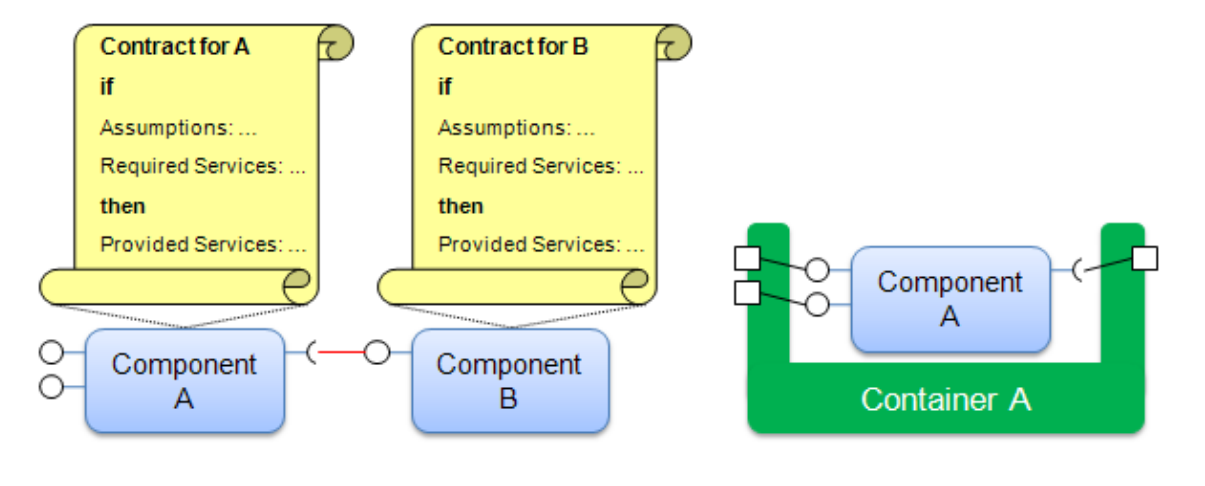
\includegraphics[height=7cm,width=15cm]{Figures/8.png}
	\caption{\textbf{Αριστερά}: Components μαζί με τα interfaces τους. \textbf{Δεξιά}: Ένας container μαζί με το component \cite{Panunzio} }	
\end{figure}

\subsection{Στόχοι της CBSD προσέγγισης}

Υπάρχουν πολλές συζητήσεις και διαφωνίες σχετικά με τι το είναι και τι δεν είναι τα components [38]. Μερικοί συγγραφείς προτιμούν να θεωρούν τα components σαν συνεκτικά πακέτα με χρήσιμη συμπεριφορά, ενώ άλλοι τα αντιμετωπίζουν σαν αναπτυσσόμενες μονάδες λογισμικού που εκτελούνται μέσα σε ένα συγκεκριμένο περιβάλλον [39]. Ανεξάρτητα από αυτές τις διαφορές, η βασική προσέγγιση της CBSD είναι η κατασκευή συστημάτων από σαφώς ορισμένα, ανεξάρτητα μεταξύ τους κομμάτια. Ωστόσο, οι ενδιαφέρουσες πτυχές της CBSD αφορούν τον τρόπο με τον οποίο επιτυγχάνεται αυτή η προσέγγιση, επιτρέποντας την ανάπτυξη των components ως κατάλληλων συνεκτικών μονάδων λειτουργικότητας και τη διευκόλυνση του σχεδιασμού και της συναρμολόγησης συστημάτων από ένα μείγμα νέων και προηγουμένων ανεπτυγμένων components [40]. Ο στόχος της δημιουργίας συστημάτων από καλά καθορισμένα κομμάτια δεν είναι κάτι καινούργιο. 

	Το ενδιαφέρον για την CBSD βασίζεται σε μια μακρά ιστορία εργασίας πάνω σε αρθρωτά συστήματα, δομημένο σχεδιασμό και πιο πρόσφατα σε αντικειμενοστραφή συστήματα [41] - [45]. Αυτά αποσκοπούσαν στην ευκολότερη ανάπτυξη και διατήρηση ευρύτερων συστημάτων χρησιμοποιώντας μια προσέγγιση “divide and conquer”. Η CBSD επεκτείνει αυτές τις ιδέες, δίνοντας έμφαση στο σχεδιασμό λύσεων με κομμάτια λειτουργικότητας που παρέχονται σαν components, προσβάσιμα σε άλλους μόνο μέσω σαφώς ορισμένων interfaces και εστιάζοντας στην ελεγχόμενη συναρμολόγηση των components χρησιμοποιώντας τεχνικές σχεδιασμού βασισμένες σε interfaces [40].


	Το πιο σημαντικό είναι ότι οι έννοιες αυτές υποστηρίζονται από μια σειρά προϊόντων που εφαρμόζουν ανοικτά πρότυπα που προσφέρουν μια υποδομή υπηρεσιών για τη δημιουργία, τη συναρμολόγηση και την εκτέλεση των components. Κατά συνέπεια, η διαδικασία ανάπτυξης εφαρμογών έχει ανασχεδιαστεί έτσι ώστε η κατασκευή λογισμικού να επιτυγχάνεται σε μεγάλο βαθμό μέσω μιας διαδικασίας επιλογής, αξιολόγησης και συναρμολόγησης των components. Τα components αποκτώνται από ένα διαφορετικό σύνολο πηγών και χρησιμοποιούνται μαζί με τοπικά σχεδιασμένο λογισμικό για την κατασκευή μιας πλήρους εφαρμογής [46].
	
\subsection{Γιατί ανάπτυξη λογισμικού με συνιστώσες}
Η ανάπτυξη λογισμικού με βάση τα components, έρχεται να δώσει σημαντικές λύσεις σε πολλές προκλήσεις που αντιμετωπίζει η βιομηχανία καθώς και οι επιχειρήσεις στην εποχή του Διαδικτύου. Αυτές οι προκλήσεις αναφέρονται στην επόμενη λίστα [40]: 

\begin{itemize}
	\item{\textbf{Πολυπλοκότητα}: Σε κάθε περίπλοκη κατάσταση υπάρχουν μερικές βασικές τεχνικές που μπορούν να χρησιμοποιηθούν για την κατανόηση και τη διαχείριση αυτής της πολυπλοκότητας. Αυτές είναι οι τεχνικές αφαίρεσης, αποσύνθεσης και σταδιακής ανάπτυξης. Κάθε λύση ανάπτυξης εφαρμογών πρέπει να παρέχει τρόπους υποστήριξης αυτών των τεχνικών.}
	\item{\textbf{Μείωση του χρόνου παράδοσης}: Η δυνατότητα έγκαιρης παράδοσης λύσεων αποτελεί ουσιαστική πτυχή κάθε έργου ανάπτυξης λογισμικού. Με τον αυξημένο ρυθμό αλλαγής της τεχνολογίας, αυτή η πτυχή γίνεται πιο σημαντική. Αυτή η ανάγκη για μειωμένο χρόνο παράδοσης συστημάτων λογισμικού αναφέρεται συχνά ως εργασίας σε “ρυθμούς Internet”.}
	\item{\textbf{Βελτίωση της συνοχής}: Τα περισσότερα συστήματα λογισμικού μοιράζονται σημαντικά χαρακτηριστικά με άλλα συστήματα που είτε έχουν αναπτυχθεί ήδη, είτε βρίσκονται στην φάση της ανάπτυξης ή δεν έχουν κατασκευαστεί ακόμα. Αν χρησιμοποιηθούν αυτά τα χαρακτηριστικά θα είναι εφικτό να βελτιωθεί η συνοχή και να μειωθεί σημαντικά το κόστος ανάπτυξης νέων συστημάτων λογισμικού. }
	\item{\textbf{Χρήση του καλύτερου στην κατηγορία}: Σε αρκετούς τομείς υπάρχουν ήδη καλά ανεπτυγμένες λύσεις που προσφέρουν ισχυρή λειτουργικότητα και απόδοση. Η αξιοποίηση αυτών των λύσεων ως μέρος μίας μεγαλύτερης προσπάθειας ανάπτυξης ενός συστήματος κρίνεται απαραίτητη. }
	\item{\textbf{Αύξηση της παραγωγικότητας}: Η έλλειψη δεξιοτήτων στον τομέα της ανάπτυξης λογισμικού έχει ως αποτέλεσμα σημαντικές καθυστερήσεις στους χρήστες συστημάτων. Οποιεσδήποτε νέες προσεγγίσεις πρέπει να βελτιώνουν την παραγωγικότητα των εργαζομένων ώστε να μπορούν να παράγουν ποιοτικά αποτελέσματα με ταχύτερους ρυθμούς. }
	\item{\textbf{Βελτίωση της ποιότητας}: Καθώς αυξάνεται το οικονομικό και ανθρώπινο αντίκτυπο μίας αποτυχίας ενός συστήματος λογισμικού, πρέπει να δοθεί ιδιαίτερη προσοχή στην ποιότητα των ανεπτυγμένων συστημάτων. Στόχος πρέπει να είναι η σωστή υποστήριξη της κατασκευής συστημάτων εξ’ αρχής, χωρίς εκτεταμένες και δαπανηρές δοκιμές και επανεγγραφή του κώδικα. }
	\item{\textbf{Αύξηση της ορατότητας στην πρόοδο του έργου}: Η διαχείριση μεγάλων έργων αποτελεί ένα εγχείρημα υψηλού κινδύνου. Για να αποφευχθεί αυτός ο κίνδυνος, πρέπει να είναι δυνατή η μεγαλύτερη ορατότητα καθ’ όλη τη διάρκεια του κύκλου ζωής του λογισμικού. Αυτό απαιτεί μια βαθμιαία προσέγγιση στην ανάπτυξη, την παράδοση και την δοκιμή κομματιών λογισμικού. }
	\item{\textbf{Υποστήριξη παράλληλου και κατανεμημένου τρόπου ανάπτυξης λογισμικού}: Οι κατανεμημένες ομάδες ανάπτυξης λογισμικού απαιτούν προσεγγίσεις που ενθαρρύνουν και επιτρέπουν την παράλληλη ανάπτυξη συστημάτων λογισμικού. Κάτι τέτοιο όμως απαιτεί ιδιαίτερη προσοχή στην διαχείριση της πολυπλοκότητας λόγω της ανάγκης διαίρεσης και επανασυγχρονισμού των αποτελεσμάτων. }
	\item{\textbf{Μείωση του κόστους συντήρησης}: Το μεγαλύτερο μέρους του κόστους ανάπτυξης ενός συστήματος προκύπτει μετά την αρχική ανάπτυξη του συστήματος. Για να μειωθεί το κόστος συντήρησης, πρέπει να είναι δυνατόν να προσδιοριστεί ευκολότερα η ανάγκη για αλλαγή, να είναι εφικτό να προβλεφθεί το αντίκτυπο που θα φέρει οποιαδήποτε προτεινόμενη αλλαγή και να εφαρμοστεί αυτή η αλλαγή στο υπάρχων σύστημα. }
	
\end{itemize}

Η παραπάνω λίστα αποτελεί ένα αποθαρρυντικό σύνολο προκλήσεων για οποιαδήποτε προσέγγιση ανάπτυξης λογισμικού. Ωστόσο, τα components και οι προσεγγίσεις που βασίζονται σε αυτά προσφέρουν την πιο ελπιδοφόρα προσπάθεια αντιμετώπισης των προκλήσεων και προσφέρουν τη βάση μιας νέας σειράς τεχνικών που υποστηρίζουν την επόμενη γενιά λύσεων που προσφέρει το λογισμικό. 

\subsection{Πλεονεκτήματα της CBSD σε σύγκριση με παραδοσιακές τεχνικές ανάπτυξης}

Αρχικά, η φιλοσοφία ανάπτυξης ενός συστήματος λογισμικού αυτών των δύο προσεγγίσεων είναι εντελώς διαφορετική. Η παραδοσιακή ανάπτυξη λογισμικού είναι ίδια με την κατασκευή από το μηδέν. Αντίθετα η CBSD προσέγγιση στηρίζεται περισσότερο στην “buy, don’t build” φιλοσοφία. Δεύτερον, η δομή του λογισμικού που αναπτύσσεται με παραδοσιακές τεχνολογίες χαρακτηρίζεται από υψηλή σύζευξη μεταξύ των επιμέρους τμημάτων του συστήματος, αλλά η CBSD προσπαθεί να κάνει την δομή του λογισμικού να έχει μία χαμηλότερη σύζευξη με σκοπό την βελτίωση της ποιότητας και της συντηρησιμότητας του κώδικα. Η τρίτη σημαντική διαφορά είναι ότι η διαδικασία ανάπτυξης ενός συστήματος λογισμικού χρησιμοποιώντας CBSD είναι εξελικτική και ταυτόχρονη. Αυτό συμβαίνει γιατί ένα σύστημα υλοποιημένο με βάση τα components στην ουσία οικοδομείται και δεν υλοποιείται από την αρχή. Σε αντίθεση με την παραδοσιακή ανάπτυξη λογισμικού, η  CBSD εστιάζει κυρίως σε δραστηριότητες που αφορούν το integration, την αναζήτηση και τον εντοπισμό των υποψήφιων components, την αξιολόγηση και την επιλογή τους βάσει των απαιτήσεων του συστήματος καθώς και των περιορισμών του έργου. Η προσέγγιση CBSD έχει πολλά πλεονεκτήματα, όπως η αποτελεσματική διαχείριση της πολυπλοκότητας, ο μειωμένος χρόνος προς την αγορά, η αυξημένη παραγωγικότητα και ο μεγαλύτερος βαθμός συνοχής και ένα ευρύτερο φάσμα χρηστικότητας. Επιπλέον, τα επαναχρησιμοποιήσιμα στοιχεία καθιστούν δυνατή τη διάσπαση της διαδικασίας ανάπτυξης εφαρμογών σε διαφορετικά μέρη, έτσι ώστε διαφορετικοί άνθρωποι ή εταιρείες να μπορούν να εκτελούν διαφορετικά μέρη της διαδικασίας.


\section{Open Services Gateway initiative (OSGi)}
\subsection{Γενικά}
Από την δεκαετία του ‘70, η οργάνωση του κώδικα σε modules θεωρείται βασική ιδιότητα για την βελτίωση της ευελιξίας, της κατανόησης και της επαναχρησιμοποίησης του [49]. Σε γενικές γραμμές, τα modules αντιστοιχούν σε μονάδες που μπορούν να εκτελέσουν μία διεργασία και μπορούν να υλοποιηθούν ανεξάρτητα, να συγκεντρωθούν και στην συνέχεια να συναρμολογηθούν κατάλληλα ώστε να υλοποιηθεί ένα σύστημα λογισμικού. Για παράδειγμα, οι κλάσεις στην Java ενθυλακώνουν τόσο δεδομένα όσο και υπηρεσίες. Μέσω της τεχνολογίας των πακέτων (packages σε όρους Java), γίνεται ομαδοποίηση και οργάνωση κλάσεων σχετικών μεταξύ τους, με αποτέλεσμα να διευκολύνεται η επαναχρησιμοποίηση. Επιπλέον, τα πακέτα μπορούν να αναπτυχθούν και να διανεμηθούν με την μορφή αρχείων JAR [50]. 

	Ωστόσο το αρθρωτό σύστημα που χρησιμοποιείται στην Java παρουσιάζει τουλάχιστον δύο προβλήματα. Πρώτον, οι μηχανισμοί απόκρυψης πληροφοριών εφαρμόζονται μόνο στο επίπεδο των κλάσεων, αλλά όχι στο επίπεδο των πακέτων και των αρχείων JAR. Για παράδειγμα, δεν είναι δυνατό να περιοριστεί η πρόσβαση σε κλάσεις με ορατότητα public που ορίζονται στα διαθέσιμα πακέτα. Η απουσία τέτοιων κανόνων ελέγχου της ορατότητας μπορεί εύκολα να οδηγήσει σε συστήματα πολύ στενά συνδεδεμένα μεταξύ τους. Από την άλλη πλευρά, το αρθρωτό σύστημα της Java είναι εγγενώς στατικό. Αυτό σημαίνει ότι τα διάφορα modules μπορούν να ενημερωθούν για τυχόν αλλαγές μόνο κατά τον χρόνο ανάπτυξης, γεγονός που απαιτεί διακοπή και επανεκκίνηση του συστήματος [50]. Ένας τέτοιος περιορισμός δημιουργεί τεράστια προβλήματα σε πολλούς τομείς όπως αυτός της βιομηχανίας όπου αναφέρεται και η παρούσα εργασία. 

	Προκειμένου να αντιμετωπιστούν οι περιορισμοί του τυποποιημένου αρθρωτού συστήματος της Java, η πρωτοβουλία  Open Services Gateway (OSGi) πρότεινε το 1999 [48] το  OSGi framework και μοντέλο προγραμματισμού, το οποίο παρέχει ένα δυναμικό αρθρωτό σύστημα με γνώμονα την παροχή υπηρεσιών για την γλώσσα προγραμματισμού Java. Σύμφωνα με τις αρχές του OSGi, τα συστήματα λογισμικού πρέπει να είναι δομημένα γύρω από ανεξάρτητα modules, τα οποία σε όρους OSGi ονομάζονται bundles, που παρέχουν σαφώς καθορισμένες υπηρεσίες. Το OSGi, καθορίζει επίσης και μια υποδομή για τον έλεγχο του κύκλου ζωής των bundles κατά τον χρόνο εκτέλεσης. Αυτή η υποδομή επιτρέπει στους προγραμματιστές να  προσθέτουν, να αφαιρούν και να αναβαθμίζουν bundles από το σύστημα δυναμικά [50]. 
	
\subsection{Η αρχιτεκτονική του OSGi}
Το OSGi παρέχει ένα γενικού σκοπού, ασφαλές και εύκολα διαχειρίσιμο framework για την Java, το οποίο υποστηρίζει την ανάπτυξη επεκτάσιμων εφαρμογών και εφαρμογών που μπορούν να μεταφορτωθούν από το διαδίκτυο, γνωστές και ως bundles. Οι συσκευές που είναι συμβατές με το OSGi μπορούν να λαμβάνουν και να εγκαθιστούν bundles τα οποία θα μπορούν να αφαιρέσουν όταν δεν θα είναι πλέον απαραίτητα. Το framework διαθετει τεχνολογίες που διαχειρίζονται την εγκατάσταση και την ενημέρωση των bundles σε ένα περιβάλλον συμβατό με το OSGi, με δυναμικό και κλιμακωτό τρόπο. Για να επιτευχθεί αυτό, οι εξαρτήσεις (dependencies) μεταξύ των bundles διαχειρίζονται λεπτομερώς από το framework [51].  

	Το OSGi έχει ένα πολυεπίπεδο μοντέλο που απεικονίζεται στην εικόνα 4.3:
	

\begin{figure}[htbp]
	\centering
		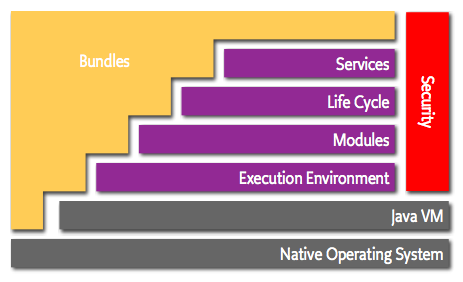
\includegraphics[height=8cm,width=14cm]{Figures/9.png}
	\caption{Τα επίπεδα της αρχιτεκτονικής του OSGi  \cite{OSGi} }	
\end{figure}

\textbf{Bundles}: Τα bundles είναι τα OSGi components που φτιάχνονται από τους προγραμματιστές. Πιο συγκεκριμένα, τα bundles είναι κανονικά .jar αρχεία που περιέχουν αρχεία για τις κλάσεις τους, άλλους πόρους όπως εικόνες, απαιτούμενα API κ. λπ., καθώς και ένα αρχείο manifest το οποίο χρησιμοποιείται για την δήλωση στατικών πληροφοριών σχετικά με το bundle, όπως τα πακέτα που εισάγει και εξάγει. Επιπλέον, κάθε bundle μπορεί να παρέχει υπηρεσίες σε άλλα bundles. Στην αρχιτεκτονική του OSGi, μια υπηρεσία είναι ένα τυπικό αντικείμενο Java που έχει καταχωρηθεί χρησιμοποιώντας έναν ή και περισσότερους τύπους διεπαφών και ιδιοτήτων που χρησιμοποιούνται για τον εντοπισμό της αντίστοιχης υπηρεσίας [50].

	\textbf{Services}: Το επίπεδο των services συνδέει τα bundles με ένα δυναμικό τρόπο προσφέροντας ένα publish-find-bind μοντέλο για τα απλά αντικείμενα Java (POJO). Είναι απαραίτητο γιατί στην Java  είναι δύσκολη η συνεργατική ανάπτυξη κώδικα με κοινή χρήση μόνο των κλάσεων. Η λύση στην Java είναι η χρήση factories που προσφέρουν δυναμική φόρτωση των κλάσεων και των στατικών στοιχείων. Για παράδειγμα αν σε μία εφαρμογή υπάρχει η ανάγκη για την δημιουργία ενός DocumentBuilderFactory θα πρέπει να γίνει κλήση στην στατική μέθοδο του factory DocumentBuilderFactory.newInstance(). Πίσω από αυτή την κλήση όμως, η μέθοδος newInstance() χρησιμοποιεί κάθε τέχνασμα του class loader ώστε να δημιουργήσει ένα νέο instance της κλάσης DocumentBuilderFactory. Αυτό αποτελεί ένα παθητικό μοντέλο. Ο κώδικας της υλοποίησης δεν μπορεί να κάνει τίποτα ώστε να αποδείξει την διαθεσιμότητά του και ο εκάστοτε χρήστης δεν μπορεί να γνωρίζει όλες τις  πιθανές υλοποιήσεις ώστε να διαλέξει την καταλληλότερη. Επιπλέον, είναι ένα στατικό μοντέλο. Μόλις μία υλοποίηση δημιουργήσει ένα νέο instance δεν μπορεί να καταστρέψει το αντικείμενο. Το χειρότερο από όλα είναι ότι αυτό ο μηχανισμός χρησιμοποιείται σε πολλά σημεία και κάθε factory έχει τους δικούς του μοναδικούς μηχανισμούς API και ρύθμισης των παραμέτρων του. Δεν υπάρχει συγκεντρωτική επισκόπηση όλων των υλοποιήσεων του εκάστοτε factory που χρησιμοποιείται. Κάτι τέτοιο δημιουργεί πολλά προβλήματα [48].

	Τη λύση σε όλα αυτά τα προβλήματα δίνει το μητρώο υπηρεσιών που παρέχει το OSGi. Ένα bundle μπορεί να δημιουργήσει ένα αντικείμενο και να το καταχωρήσει στο μητρώο υπηρεσιών κάτω από μία ή περισσότερες διεπαφές. Άλλα bundles μπορούν να μεταβούν στο μητρώο και να βρουν όλα τα αντικείμενα που είναι καταχωρημένα κάτω από μία διεπαφή ή κλάση. Για παράδειγμα, ένα bundle μπορεί να παρέχει μία συγκεκριμένη υλοποίηση του DocumentBuilderIf. Όταν ξεκινάει, δημιουργεί ένα instance του αντικειμένου DocumentBuilderImpl και το καταχωρεί στο μητρώο υπηρεσιών. Ένα bundle που χρειάζεται ένα αντικείμενο DocumentBuilder μπορεί να μεταβεί στο μητρώο και να ζητήσει όλες τις διαθέσιμες υπηρεσίες που υλοποιούν το DocumentBuilderIf. Ακόμα καλύτερα ένα bundle μπορεί να περιμένει μία υπηρεσία να εμφανιστεί και να πάρει μία κλήση πίσω (call back) [48]. 

	Επομένως, ένα bundle μπορεί να καταχωρίσει μία υπηρεσία στο μητρώο, να λάβει μία υπηρεσία που είναι ήδη καταχωρημένη και να περιμένει μία υπηρεσία να εμφανιστεί ή να εξαφανιστεί. Οποιοσδήποτε αριθμός bundles μπορεί να καταχωρίσει την ίδια υπηρεσία και οποιοσδήποτε αριθμός bundles μπορεί να λάβει την ίδια υπηρεσία [48]. Αυτή η λειτουργικότητα εμφανίζεται στην εικόνα 4.4.

	Σύμφωνα με όσα αναφέρθηκαν, είναι εύλογο το ερώτημα πως διαχωρίζονται οι υπηρεσίες αν πολλά bundles έχουν καταχωρήσει την ίδια υπηρεσία. Αρχικά, σε πολλές περιπτώσεις δεν είναι σημαντικό να γίνει διάκριση της υπηρεσίας από ένα συγκεκριμένο bundle. Σε περίπτωση όμως που κάτι τέτοιο κριθεί αναγκαίο το OSGi παρέχει τις ιδιότητες. Κάθε υπηρεσία που καταχωρείται έχει ένα σύνολο από τυπικές και προσαρμοσμένες ιδιότητες. Επιπλέον, υπάρχει μία συγκεκριμένη γλώσσα που μπορεί να φιλτράρει τις υπηρεσίες που παρέχονται και να διαλέξει μόνο αυτές που χρειάζεται το συγκεκριμένο bundle. Οι ιδιότητες μπορούν να χρησιμοποιηθούν για να επιλεχθεί η κατάλληλη υπηρεσία ή να παίξουν και άλλους ρόλους σε επίπεδο εφαρμογής [48].
	
\begin{figure}[htbp]
	\centering
		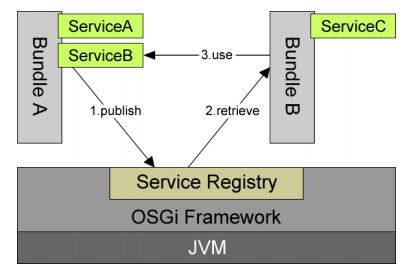
\includegraphics[height=7cm,width=11cm]{Figures/10.png}
	\caption{Το μητρώο υπηρεσίων του OSGi \cite{Tavares} }	
\end{figure}

Οι υπηρεσίες είναι δυναμικές. Αυτό σημαίνει ότι ένα bundle μπορεί να αποφασίσει να  αποσύρει μία υπηρεσία της από το μητρώο, ενώ άλλα bundles εξακολουθούν να χρησιμοποιούν αυτή την υπηρεσία. Τα bundles που χρησιμοποιούν μια τέτοια υπηρεσία πρέπει να διασφαλίζουν ότι δεν χρησιμοποιούν πλέον το αντικείμενο αυτής της υπηρεσίας και να διαγράψουν οποιοδήποτε reference έχουν σε αυτή την υπηρεσία. Αυτό ίσως ακούγεται σαν να επιφέρει σημαντική πολυπλοκότητα αλλά έχουν υλοποιηθεί αρκετές τεχνολογίες οι οποίες λύνουν αυτό το πρόβλημα και επιφέρουν σημαντικά πλεονεκτήματα. Τέτοιες είναι το Service Tracker και τα Declarative Services τα οποία χρησιμοποιήθηκαν στην παρούσα εργασία. Αυτή η δυναμική των υπηρεσιών καθιστά εφικτή την εγκατάσταση και απεγκατάσταση bundles κατά την διάρκεια του run-time και τα υπόλοιπα bundles του συστήματος να μπορούν να προσαρμοστούν. Δηλαδή στην δική μας υλοποίηση μπορούμε να αλλάξουμε το bundle του Valve κατά την διάρκεια που το liqueur θερμαίνεται και το σύστημα να συνεχίζει να δουλεύει κανονικά. 


\textbf{Life-Cycle}: Αποτελεί ένα API για την διαχείριση του κύκλου ζωής των bundles, δηλαδή την εγκατάσταση, την έναρξη, την αναβάθμιση, την διακοπή και την απεγκατάσταση των bundles. Επιπρόσθετα,  παρέχει ένα περιεκτικό API για τα events για να επιτρέπει σε ένα bundle διαχείρισης να ελέγχει τις λειτουργίες του OSGi framework. To επίπεδο Life-Cycle απαιτεί το Module επίπεδο, ενώ το επίπεδο Security δεν είναι απαραίτητο [51]. 

\textbf{Modules}:  Η πλατφόρμα Java προσφέρει περιορισμένη υποστήριξη για τον διαχωρισμό σε πακέτα, την ανάπτυξη και τον έλεγχο εφαρμογών και components που βασίζονται στην γλώσσα Java. Εξαιτίας αυτού, πολλά έργα που βασίζονται σε Java, όπως τα  Jboss και Netbeans, έχουν καταφύγει στην δημιουργία προσαρμοσμένων αντίστοιχων επιπέδων (module layer) με εξειδικευμένους class loaders ώστε να παρέχουν καλύτερη υποστήριξη στην ανάπτυξη, τον διαχωρισμό σε πακέτα και τον έλεγχο εφαρμογών. Το OSGi παρέχει μια γενική και τυποποιημένη λύση για το modularization εφαρμογών.  

	Πιο αναλυτικά, το OSGi ορίζει μία μονάδα (module) το bundle. Ένα bundle αποτελείται από κλάσεις Java και άλλους πόρους, οι οποίοι μαζί μπορούν να παρέχουν λειτουργίες στους τελικούς χρήστες. Τα bundles μπορούν να μοιράζονται πακέτα με άλλα bundles. Στο OSGi τα bundles είναι οι μοναδικές οντότητες για την ανάπτυξη εφαρμογών. Ένα bundle αναπτύσσεται σαν ένα αρχείο .jar. Τα αρχεία .jar συνήθως χρησιμοποιούνται για την αποθήκευση των εφαρμογών και των πόρων τους σε μία τυπική μορφή αρχείου .zip. Ωστόσο, υπάρχει ένας ειδικός τύπος ΜΙΜΕ που προορίζεται για τα OSGi bundles που χρησιμοποιείται για να διακρίνονται τα bundles από κανονικά αρχεία .jar [51]. 

\textbf{Security}: Είναι ένα προαιρετικό επίπεδο που βασίζεται στην αρχιτεκτονική ασφάλειας Java 2. Παρέχει την υποδομή για την ανάπτυξη και την διαχείριση εφαρμογών που πρέπει να εκτελούνται σε ελεγχόμενα και ασφαλή περιβάλλοντα [51]. 

\subsection{Πλεονεκτήματα του OSGi}

Ο βασικός λόγος που το OSGi είναι τόσο επιτυχημένο είναι ότι παρέχει ένα πολύ ώριμο σύστημα για την ανάπτυξη εφαρμογών με την χρήση component, που λειτουργεί σε έναν εκπληκτικό αριθμό περιβάλλοντων. Το OSGi χρησιμοποιείται σε ιδιαίτερα περίπλοκες εφαρμογές όπως περιβάλλοντα ανάπτυξης κώδικα (IDEs), διακομιστές εφαρμογών, gateways καθώς και σε εφαρμογές βιομηχανικού αυτοματισμού. 

	Τα πλεονεκτήματα που παρέχει το OSGi σύμφωνα με το [48] αναφέρονται παρακάτω: 
	
\begin{itemize}
	\item{\textbf{Το OSGi αρχικά δημιουργήθηκε για το ΙοΤ}: Από την αρχή το OSGi είχε σχεδιαστεί με γνώμονα συσκευές με χαμηλή επεξεργαστική ισχύ και μνήμη RAM. Οι συσκευές σήμερα  έχουν μεγαλύτερη επεξεργαστική ισχύ και καλύτερους πόρους. Εξαιτίας αυτού δημιουργήθηκαν εξελιγμένες εφαρμογές και λύσεις καθώς και ακμάζοντα οικοσυστήματα οργανισμών που συνεισφέρουν στην ανάπτυξη λογισμικού. Τέτοια οικοσυστήματα μπορούν να βρεθούν σε ποικίλες αγορές όπως την αγορά των “έξυπνων σπιτιών”, των “έξυπνων” αυτοκινήτων και της Industrie 4.0. Το βιομηχανικό σύστημα παραγωγής λικέρ που χρησιμοποιήθηκε ως μελέτη στην παρούσα διπλωματική εργασία υιοθέτησε σαν βάση το OSGi για την ανάπτυξη του συστήματος παραγωγής myLiquerProduction, το οποίο εκμεταλλεύεται τις τεχνολογίες του ΙοΤ για να επιτρέπει στους τελικούς χρήστες να παράγουν προσαρμοσμένους τύπους λικέρ. Το smartSilo υλοποιήθηκε χρησιμοποιώντας τον hardware προσομοιωτή Silo που είχε αναπτυχθεί σε προηγούμενη διπλωματική εργασία και έναν Controller σε επίπεδο λογισμικού που τρέχει σε Raspberry Pi και αναπτύχθηκε κάτω από το Apache Felix Framework το οποίο αποτελεί μία υλοποίηση ανοιχτού κώδικα του OSGi. }
	\item{\textbf{Μειωμένη πολυπλοκότητα}: Η ανάπτυξη εφαρμογών με το OSGi σημαίνει την ανάπτυξη bundles. Τα bundles κρύβουν τα εσωτερικά στοιχεία τους από τα υπόλοιπα bundles και επικοινωνούν μεταξύ τους μέσω σαφώς καθορισμένων υπηρεσιών. Η απόκρυψη των εσωτερικών στοιχείων προσδίδει μεγαλύτερη ελευθερία στην ανάπτυξη και ευκολία σε οποιαδήποτε αλλαγή που θα επέλθει αργότερα. Κάτι τέτοιο όχι μόνο μειώνει των αριθμό των σφαλμάτων, αλλά κάνει την διαδικασία ανάπτυξης των bundles πιο απλή καθώς κάθε bundle θα υλοποιεί ένα κομμάτι λειτουργικότητας μέσω σαφώς καθορισμένων interfaces. Κάθε component στην συγκεκριμένη εργασία αντιπροσωπεύει αντικείμενα πραγματικού κόσμου του παραδείγματος που υλοποιήθηκε σαν μελέτη, αλλά σε τομέα λογισμικού.}
	\item{\textbf{Επαναχρησιμοποίηση}: Το μοντέλο για τα components που παρέχει το OSGi καθιστά εύκολη τη χρήση πολλών components, που έχουν αναπτυχθεί από τρίτους, σε μία εφαρμογή. Στην υλοποίηση μας χρησιμοποιήθηκαν πολλά τέτοια bundles όπως το Californium for OSGi που είναι μία υλοποίηση του πρωτοκόλλου CoAP σε Java, ο Pax Logger που χρησιμοποιήθηκε σαν logger, η βιβλιοθήκη Pi4J που είναι υπεύθυνη για τον έλεγχο τον General Purpose Inputs Outputs (GPIO) του Raspberry Pi κλπ. }
	\item{\textbf{Δυναμικότητα}: Το μοντέλο του OSGi είναι δυναμικό. Τα διάφορα bundles μπορούν να εγκαθιστώνται, να αναβαθμίζονται, να σταματάνε και να ξεκινούν χωρίς να πρέπει να σταματήσει να λειτουργεί ολόκληρο το σύστημα. Οι περισσότεροι προγραμματιστές δεν θεωρούν ότι κάτι τέτοιο είναι αξιόπιστο και για αυτό το λόγο δεν το χρησιμοποιούν σε πραγματικά περιβάλλοντα. Επιπλέον, στον κόσμο του OSGi οι υπηρεσίες που παρέχει το κάθε bundle μπορεί ανά πάσα στιγμή να μην υπάρχουν. Ωστόσο και ο πραγματικός κόσμος είναι δυναμικός και οι δυναμικές υπηρεσίες που έρχονται και φεύγουν καθιστούν τις δυναμικές υπηρεσίες του OSGi ένα τέλειο μηχανισμό που δίνει λύσει σε πολλά σενάρια πραγματικού κόσμου. Αυτή η δυναμικότητα όμως εξηγείται καλύτερα μέσω ενός παραδείγματος. Στην μελέτη που έγινε στην παρούσα εργασία μία υπηρεσία θα μπορούσε να είναι το άνοιγμα μίας βάνας ενός σιλό. Έστω ότι παρουσιάζεται ένα πρόβλημα και το λογισμικό του controller για τη συγκεκριμένη λειτουργία του συστήματος παρουσιάζει ένα σφάλμα. Τότε μπορεί να αλλαχθεί το bundle που παρέχει την υπηρεσία για το άνοιγμα της βάνας με κάποιο bundle που διορθώνει το πρόβλημα χωρίς να πρέπει να σταματήσει η λειτουργία ολόκληρου του συστήματος. Μόλις το νέο bundle εγκατασταθεί στο περιβάλλον του OSGi και να καταχωρηθεί η νέα υπηρεσία που αυτό παρέχει. Έτσι ο controller βρίσκει τη νέα υπηρεσία και την επόμενη φορά που θα γίνει μία κλήση σε αυτή την μέθοδο θα χρησιμοποιηθεί αυτή. Το συγκεκριμένο παράδειγμα ελέγχθηκε και στην υλοποίηση μας. }
	\item{\textbf{Απλότητα}: Το OSGi είναι εξαιρετικά απλό παρά την διαχείριση των εξαρτήσεων μεταξύ των bundles και της δυναμικότητας που παρέχει. Ο κώδικας σε ένα bundle συμβατό με το OSGi μοιάζει σχεδόν με τον κλασικό κώδικα Java. Ένας συνδυασμός από annotations (Declarative Services) δηλώνουν στο framework πως να χρησιμοποιήσει τον δυναμικό χαρακτήρα του OSGi, καθώς και το ενημερώνουν για τις διάφορες εξαρτήσεις μεταξύ των bundles. Αυτό το πολύ απλό μοντέλο επιτρέπει τη σταδιακή χρήση πιο προηγμένων λειτουργιών. }
\end{itemize}


\subsection{Υλοποιήσεις του OSGi}

Το OSGi είναι ένα τυποποιημένο σύστημα για modules και μία πλατφόρμα υπηρεσιών για την γλώσσα προγραμματισμού Java. Τα πρότυπα του OSGi ορίζονται από την OSGi Alliance και δημοσιεύονται από την ίδια πρωτοβουλία [48]. Αυτή η ενότητα περιέχει μια επισκόπηση των διαθέσιμων υλοποιήσεων του OSGi, τόσο εμπορικές όσο και ανοιχτού κώδικα. Μία γρήγορη επισκόπηση απεικονίζεται στον πίνακα 4.1, που αποτελεί μία τροποποίηση του πίνακα που βρίσκετε στην [53] . 

\begin{table}[h]
\centering
\resizebox{\textwidth}{!}{%
\begin{tabular}{|l|c|c|c|c|}
\hline
\multicolumn{1}{|c|}{} & \textbf{\begin{tabular}[c]{@{}c@{}}Apache Felix\\ (4.4) \\ Open Source\end{tabular}} & \textbf{\begin{tabular}[c]{@{}c@{}}Eclipse Equinox\\ (4.5)\\ Open Source\end{tabular}} & \textbf{\begin{tabular}[c]{@{}c@{}}Knoplerfish\\ (5.1)\\ Open Source\end{tabular}} & \textbf{\begin{tabular}[c]{@{}c@{}}ProSyst\\ (SDK 7.3)\\ Commercial\end{tabular}} \\ \hline
Security (v1.8) & \cellcolor[HTML]{F56B00}1.7 & \cellcolor[HTML]{32CB00}1.8 & \cellcolor[HTML]{F56B00}1.7 & \cellcolor[HTML]{F56B00}1.5 \\ \hline
Core Framework (v6.0) & \cellcolor[HTML]{32CB00}6 & \cellcolor[HTML]{32CB00}6 & \cellcolor[HTML]{32CB00}6 & \cellcolor[HTML]{32CB00}6 \\ \hline
Package Admin Service (v1.2) & \cellcolor[HTML]{32CB00}1.2 & \cellcolor[HTML]{32CB00}1.2 & \cellcolor[HTML]{32CB00}1.2 & \cellcolor[HTML]{32CB00}1.2 \\ \hline
Start Level Service (v1.1) & \cellcolor[HTML]{32CB00}1.1 & \cellcolor[HTML]{32CB00}1.1 & \cellcolor[HTML]{32CB00}1.2 & \cellcolor[HTML]{32CB00}1.2 \\ \hline
Conditional Admin Service (v1.1) & \cellcolor[HTML]{32CB00}1.1 & \cellcolor[HTML]{32CB00}1.1 & \cellcolor[HTML]{32CB00}1.1 & \cellcolor[HTML]{32CB00}1.1 \\ \hline
Permission Admin Service (v1.2) & \cellcolor[HTML]{32CB00}1.2 & \cellcolor[HTML]{32CB00}1.2 & \cellcolor[HTML]{32CB00}1.2 & \cellcolor[HTML]{32CB00}1.2 \\ \hline
URL Handler Service (v1.0) & \cellcolor[HTML]{32CB00}1 & \cellcolor[HTML]{32CB00}1 & \cellcolor[HTML]{32CB00}1 & \cellcolor[HTML]{32CB00}1 \\ \hline
Log	Service (v1.3) & \cellcolor[HTML]{32CB00}1.3 & \cellcolor[HTML]{32CB00}1.3 & \cellcolor[HTML]{32CB00}1.3 & \cellcolor[HTML]{32CB00}1.3 \\ \hline
HTTP Service (v1.2) & \cellcolor[HTML]{32CB00}1.2 & \cellcolor[HTML]{32CB00}1.2 & \cellcolor[HTML]{32CB00}1.2 & \cellcolor[HTML]{32CB00}1.2 \\ \hline
Device Access Service (v1.1) & \cellcolor[HTML]{FE0000}x & \cellcolor[HTML]{32CB00}1.1 & \cellcolor[HTML]{32CB00}1.1 & \cellcolor[HTML]{32CB00}1.1 \\ \hline
Configuration Admin Service (v1.5) & \cellcolor[HTML]{F56B00}1.3 & \cellcolor[HTML]{F56B00}1.3 & \cellcolor[HTML]{32CB00}1.5 & \cellcolor[HTML]{F56B00}1.3 \\ \hline
Meta-type Service (v1.2) & \cellcolor[HTML]{F56B00}1.1 & \cellcolor[HTML]{32CB00}1.2 & \cellcolor[HTML]{32CB00}1.2 & \cellcolor[HTML]{F56B00}1.1 \\ \hline
Preference Service (v1.1) & \cellcolor[HTML]{32CB00}1.1 & \cellcolor[HTML]{32CB00}1.1 & \cellcolor[HTML]{32CB00}1.1 & \cellcolor[HTML]{32CB00}1.1 \\ \hline
User Admin Service (v1.1) & \cellcolor[HTML]{32CB00}1.1 & \cellcolor[HTML]{32CB00}1.1 & \cellcolor[HTML]{32CB00}1.1 & \cellcolor[HTML]{FE0000}x \\ \hline
Wire Admin Service (v1.0) & \cellcolor[HTML]{32CB00}1 & \cellcolor[HTML]{FE0000}x & \cellcolor[HTML]{32CB00}1 & \cellcolor[HTML]{32CB00}1 \\ \hline
IO Connector Service (v1.3) & \cellcolor[HTML]{32CB00}1.3 & \cellcolor[HTML]{FE0000}x & \cellcolor[HTML]{32CB00}1.3 & \cellcolor[HTML]{32CB00}1.3 \\ \hline
Initial Provisioning Service (v1.2) & \cellcolor[HTML]{32CB00}1.2 & \cellcolor[HTML]{FE0000}x & \cellcolor[HTML]{32CB00}1.2 & \cellcolor[HTML]{32CB00}1.2 \\ \hline
UPnP Device Service (v1.2) & \cellcolor[HTML]{F56B00}1.1 & \cellcolor[HTML]{FE0000}x & \cellcolor[HTML]{32CB00}1.2 & \cellcolor[HTML]{F56B00}1.1 \\ \hline
Declarative Service (v1.2) & \cellcolor[HTML]{32CB00}1.2 & \cellcolor[HTML]{32CB00}1.2 & \cellcolor[HTML]{32CB00}1.2 & \cellcolor[HTML]{F56B00}1.1 \\ \hline
Event Admin Service (v1.3) & \cellcolor[HTML]{32CB00}1.3 & \cellcolor[HTML]{32CB00}1.3 & \cellcolor[HTML]{32CB00}1.3 & \cellcolor[HTML]{F56B00}1.2 \\ \hline
Deployment Admin Service (v1.1) & \cellcolor[HTML]{32CB00}1.1 & \cellcolor[HTML]{FE0000}x & \cellcolor[HTML]{32CB00}1.1 & \cellcolor[HTML]{32CB00}1.1 \\ \hline
\end{tabular}%
}
\caption{Διαθέσιμες υλοποιήσεις του OSGi και η έκδοση των modules που υποστηρίζουν}
\label{my-label}
\end{table}

Όπως φαίνεται στον πίνακα 4.1 συγκρίνονται τέσσερις υλοποιήσεις του OSGi, οι τρεις εκ των οποίων είναι ανοιχτού κώδικα. Το \textbf{Apache Felix} αποτελεί μία κοινοτική προσπάθεια για την υλοποίηση του OSGi Framework και άλλων τεχνολογιών που σχετίζονται με το OSGi υπό την άδεια Apache [52]. Αποτελεί την βασική επιλογή των προγραμματιστών που ασχολούνται με το OSGi. Αποτελεί την πιο καθαρή υλοποίηση του OSGi γι’ αυτό και τα modules του που παρέχουν διάφορες υπηρεσίες των προδιαγραφών του OSGi μπορούν να λειτουργήσουν άψογα ακόμα και αν εγκατασταθούν σε κάποια άλλη υλοποίηση. 

	Το \textbf{Knoplerfish} είναι μία υλοποίηση του OSGi που υποστηρίζεται και αναπτύσσεται από την Makewave [54]. Είναι η πιο απλή υλοποίηση του OSGi καθώς έχει σχεδιαστεί για ενσωματωμένα συστήματα και για περιβάλλοντα με περιορισμένους πόρους. Σύμφωνα με την [53], σε μία σύγκριση των παραπάνω υλοποιήσεων αυτή του Knoplerfish αποδείχτηκε η πιο γρήγορη, όταν οι δοκιμές και οι μετρήσεις έγιναν πάνω σε ένα Raspberry Pi. Η συγκεκριμένη υλοποίηση έχει αναπτυχθεί πάνω στο Apache Felix. 

	Το \textbf{Equinox} είναι μία εφαρμογή των προδιαγραφών που ορίζονται από το OSGi, αλλά παρέχει και ένα σύνολο από bundles που υλοποιούν διάφορες προαιρετικές υπηρεσίες του OSGi καθώς και μία υποδομή για τη λειτουργία συστημάτων που βασίζονται στο OSGi. Υποστηρίζεται και αναπτύσσεται από το Eclipse project [55].

	Τέλος, η \textbf{Prosyst} είναι μία από τις πρώτες εταιρείες που συμμετείχαν στην πρωτοβουλία OSGi Alliance και έχει συμβάλλει σημαντικά στην ανάπτυξη των προδιαγραφών του OSGi. Πλέον εστιάζει αποκλειστικά στην ανάπτυξη λογισμικού και λύσεων σχετικών με το OSGi, όπως frameworks, bundles, την υλοποίηση του OSGi που μελετήθηκε σε αυτή την ενότητα. Οι λύσεις που παρέχει χρησιμοποιούνται από συσκευές για το Smart Home, κατασκευαστές αυτοκινήτων, κατασκευαστές κινητών τηλεφώνων κ.α [56]. 

	Στην παρούσα μελέτη, χρησιμοποιήθηκε η υλοποίηση που μας παρέχει το Apache Felix. Αυτό έγινε κυρίως γιατί σκοπός ήταν να δημιουργηθεί ένα περιβάλλον OSGi εξ’ ολοκλήρου από την αρχή ώστε να υπάρχει έλεγχος σε οποιοδήποτε bundle έτρεχε κατά την διάρκεια του run time. Ένα άλλος λόγος που οδηγηθήκαμε σε αυτή την απόφαση ήταν και η υλοποίηση των Core προδιαγραφών του OSGi καθώς την περίοδο που εκπονήθηκε η εργασία οι υπόλοιπες υλοποιήσεις δεν παρείχαν την τελευταία έκδοση αυτών των προδιαγραφών αλλά παρείχαν κάποια προηγούμενη. Αξίζει να σημειωθεί ότι κατά την διάρκεια της εργασίας χρησιμοποιήθηκε και το \textbf{Apache Karaf }το οποίο είναι ένας container βασισμένος σε OSGi χτισμένος πάνω στο Apache Felix. Το Karaf παρέχει πολλές υπηρεσίες χωρίς να χρειάζεται να εγκατασταθούν μία προς μία τις οποίες χρειαστήκαμε στην υλοποίηση μας. Τέτοιες είναι υπηρεσίες όπως οι File Install, Declarative Services, Jetty Server, Felix Webconsole και άλλες που θα αναφερθούν στην συνέχεια. Ωστόσο, στην τελική υλοποίηση χρησιμοποιήσαμε το Apache Felix καθώς ήταν πιο ελαφρύ από το Karaf και μας παρείχε την ίδια λειτουργικότητα.

\addtocontents{toc}{\vspace{2em}}
\chapter{Το Liqueur Plant Σύστημα Παραγωγής} % Main chapter title

\label{Chapter5} 

Στο [56] περιγράφεται ένα σύστημα παραγωγής liqueur και ένα σύστημα ελέγχου του βιομηχανικού συστήματος παραγωγής, βασισμένο σε PLC’s προγραμματισμένα σε γλώσσες προτύπου IEC61131. Στα πλαίσια της παρούσας διπλωματικής εργασίας αναπτύχθηκε για το ίδιο σύστημα παραγωγής ένα σύστημα ελέγχου βασισμένο σε τεχνολογίες ΙοΤ ακολουθώντας την component-based προσέγγιση για την ανάπτυξη του λογισμικού. Στο εξής θα γίνονται αναφορές σε αυτό το βιομηχανικό σύστημα παραγωγής σαν LPPS. Το συγκεκριμένο βιομηχανικό σύστημα έχει μελετηθεί ήδη και στις [57], [58], [59]. Έτσι μελετήθηκε, σχεδιάστηκε και υλοποιήθηκε ένα σύστημα παραγωγής  δύο τύπων liqueur βασισμένο στις προδιαγραφές του LPPS, το οποίο φαίνεται στην εικόνα 5.1:


\begin{figure}[htbp]
	\centering
		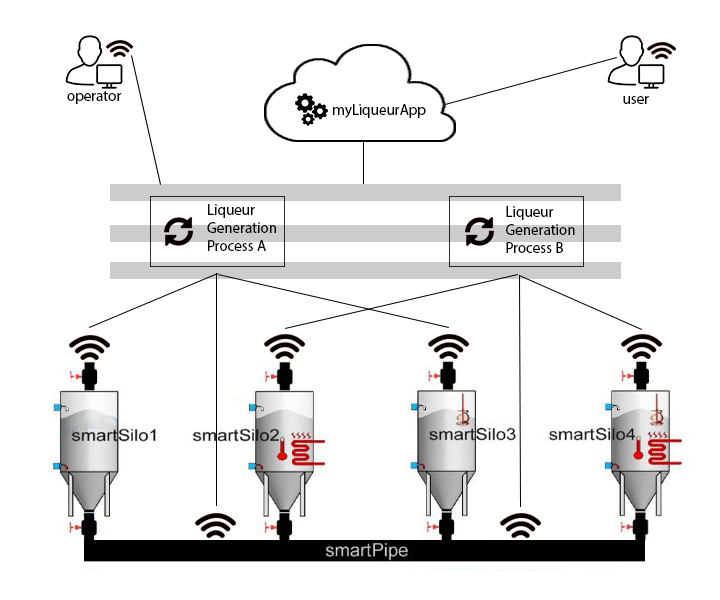
\includegraphics[height=11cm,width=15cm]{Figures/11.png}
	\caption{Σχηματική αναπαράσταση του συστήματος παραγωγής liqueur \cite{Thrampo3} }	
\end{figure}


	Το σύστημα αποτελείται από τέσσερα σιλό συνδεδεμένα μεταξύ τους με ένα σωλήνα. Κάθε ένα σιλό αποτελείται από μία βαλβίδα εισαγωγής και μία βαλβίδα εξαγωγής υγρού, καθώς και από δύο αισθητήρες για τον έλεγχο της παρουσίας υγρού, έναν στο πάνω μέρος ο οποίος ανιχνεύει αν το σιλό έχει γεμίσει  και έναν στο κάτω μέρος που ανιχνεύει αν το σιλό έχει αδειάσει. Επιπλέον, δύο από τα σιλό, το smartSilo2 και το smartSilo4, έχουν ένα στοιχείο θέρμανσης του υγρού και έναν αισθητήρα που ανιχνεύει την θερμοκρασία του υγρού. Τα smartSilo3 και smartSilo4 περιλαμβάνουν από ένα στοιχείο μίξης του υγρού. 

	Στο συγκεκριμένο σύστημα παράγονται δύο τύποι liqueur ακολουθώντας την εξής διαδικασία: 

\begin{itemize}
	\item{\textbf{Παραγωγή τύπου liqueur A}: Για να ξεκινήσει η παραγωγή του liqueur τύπου Α, το σιλό 1 γεμίζει με υγρό. Μόλις γεμίσει θα πρέπει να μεταφερθεί το υγρό αυτό μέσω του σωλήνα στο σιλό 4. Στη συνέχεια μόλις μεταφερθεί όλο το υγρό στο σιλό 4, θερμαίνεται μέχρι να φτάσει σε μία επιθυμητή θερμοκρασία και τέλος αναδεύεται για ένα συγκεκριμένο χρονικό διάστημα με την χρήση του στοιχείου μίξης του σιλό 4. Τέλος το υγρό μεταφέρεται σε άλλο σημείο παραγωγής μέσω της βαλβίδας εξαγωγής του σιλό 4. }
	\item{\textbf{Παραγωγή τύπου liqueur B}: Για την παραγωγή liqueur τύπου Β το σιλό 2 γεμίζει με υγρό. Μόλις γεμίσει το υγρό θερμαίνεται μέχρι να φτάσει σε μία επιθυμητή θερμοκρασία. Στη συνέχεια θα πρέπει να μεταφερθεί μέσω του σωλήνα στο σιλό 3. Αφού μεταφερθεί το υγρό αναδεύεται για ένα συγκεκριμένο χρονικό διάστημα μέσω του στοιχείου μείξης του σιλό 3. Τέλος, το υγρό μεταφέρεται σε άλλο σημείο παραγωγής μέσω της βαλβίδας εξαγωγής του σιλό 3. }
\end{itemize}

Οι δύο τύποι liqueur που μπορούν να παραχθούν καθώς και η διαδικασίες που ακολουθούνται για την παραγωγή τους είναι ανεξάρτητες και μπορούν να γίνουν ταυτόχρονα. Αλλά θα πρέπει να ληφθούν υπόψιν οι εξής περιορισμοί. Ο σωλήνας είναι κοινός πόρος και μπορεί να υποστηρίξει μία μεταφορά κάθε φορά. Δηλαδή μεταφορά υγρού από το σιλό 1 στο σιλό 4 ή μεταφορά υγρού από το σιλό 2 στο σιλό 3. Επιπλέον, υπάρχει και περιορισμός στην κατανάλωση ισχύος και γι’ αυτό θα πρέπει να λειτουργεί μόνο ένας αναδευτήρας κάθε φορά και όχι και οι δύο ταυτόχρονα. 

Οποιοσδήποτε χρήστης του myLiqueurApp θα μπορεί να ορίζει τον τύπο του liqueur που θέλει καθώς και τις διάφορες ιδιότητες του, δηλαδή σε ποια θερμοκρασία πρέπει να θερμανθεί και για πόση ώρα θα πρέπει να αναδευτεί καθώς και την ποσότητα που θέλει. Επιπλέον, θεωρούμε ότι τα σιλό απέχουν αρκετά μεταξύ τους ώστε να έχει σημασία η χρήση τεχνολογιών IoT για την επικοινωνία τους.
\addtocontents{toc}{\vspace{2em}}
\chapter{Σχεδιασμός του συστήματος} % Main chapter title

\label{Chapter6} 

\section{Εισαγωγή}
Στο κεφάλαιο αυτό θα γίνει μία περιγραφή του σχεδιασμού του συστήματος ελέγχου του κάθε σιλό του LPPS ξεχωριστά. Για να γίνει αυτό και το κάθε σιλό να είναι σε θέση να αναβαθμιστεί χρησιμοποιώντας τεχνολογίες ΙοΤ είναι απαραίτητη η ενσωμάτωση ενός μικροϋπολογιστή με δυνατότητες δικτύωσης σε κάθε σιλό. Από εδώ και στο εξής ένα τέτοιο σύστημα, δηλαδή τα μηχανικά στοιχεία ενός σιλό σε συνεργασία με τον μικροϋπολογιστή, θα καλείται Industrial Automation Thing (IAT). 

	Αυτοί οι μικροϋπολογιστές, αποτελούν τους LwM2M clients του συστήματος και θα παρέχουν υπηρεσίες στο περιβάλλον τους που μπορεί να τις αξιοποιήσει ένας LwM2M server ώστε να επιτυγχάνεται η παραγωγή liqueur που είναι και το ζητούμενο. 
	
Για τον σχεδιασμό του συστήματος χρησιμοποιήθηκε η γλώσσα UML, που είναι μια γλώσσα γενικής χρήσης, ανάπτυξης και μοντελοποίησης στον τομέα της μηχανικής λογισμικού και παρέχει έναν τυποποιημένο τρόπο απεικόνισης του σχεδιασμού ενός συστήματος. Η υλοποίηση των διαγραμμάτων UML έγινε με την βοήθεια του εργαλείου Papyrus. 
	
\section{Σχεδιασμός του API του Industrial Automation Thing}

Για να γίνει ο σχεδιασμός του API του ΙΑΤ έπρεπε αρχικά να ληφθούν υπόψιν όλα τα κρίσιμα τμήματα των διεργασιών που μπορεί να εκτελέσει ένα σιλό. Τα κρίσιμα τμήματα που σημειώθηκαν και σύμφωνα με τα οποία έγινε ο σχεδιασμός του συστήματος είναι τα παρακάτω: 

\begin{itemize}
	\item{Όταν ένα σιλό γεμίζει με υγρό πρέπει οι πάνω βαλβίδα να κλείσει αμέσως μόλις ανιχνευθεί υγρό. Αν δεν γίνει αυτό το σιλό μπορεί να συνεχίζει να γεμίζει πέρα από το επιθυμητό επίπεδο. }
	\item{Όταν ένα σιλό αδειάζει από υγρό η κάτω βαλβίδα πρέπει να κλείσει αμέσως μόλις ο κάτω αισθητήρας του σιλό ανιχνεύσει απουσία υγρού. }
	\item{Όταν ένα σιλό θερμανθεί μέχρι μία συγκεκριμένη θερμοκρασία τότε το στοιχείο θέρμανσης του σιλό πρέπει να απενεργοποιηθεί άμεσα ώστε να μην ξεπεραστεί η θερμοκρασία αυτή.}
	\item{Όταν ένα σιλό έχει αναδευτεί για το επιθυμητό χρονικό διάστημα το στοιχείο μίξης πρέπει να απενεργοποιηθεί αλλιώς μπορεί να μην έχουμε το επιθυμητό αποτέλεσμα στον τελικό προϊόν.}
\end{itemize}


	Παρατηρείται ότι οι κρίσιμες λειτουργίες αφορούν τα μηχανικά στοιχεία και τις λειτουργίες μόνο ενός σιλό και έτσι δεν χρειάζεται επιπλέον γνώση οποιασδήποτε πληροφορίας ή αλληλεπίδρασης με το περιβάλλον του. Αυτό σε συνδυασμό με την παραδοχή ότι το κάθε σιλό βρίσκεται σε μεγάλη απόσταση από τα υπόλοιπα καθιστά σαφές ότι θα πρέπει να υπάρχει ενσωματωμένος ένας μικροϋπολογιστής σε κάθε σιλό ξεχωριστά και ότι το κάθε σιλό θα αποτελεί και έναν LwM2M client. Έτσι σύμφωνα με τις προδιαγραφές του OMA LwM2M ορίστηκαν κάποια συγκεκριμένα LwM2M objects καθώς και resources, μέσω των οποίων γίνεται η πρόσβαση στις υπηρεσίες που παρέχει το κάθε σιλό. Αυτά αναλύονται καλύτερα στην επόμενη ενότητα.
	
\section{Περιγραφή των LwM2M objects και resources}
Παρακάτω αναφέρονται και περιγράφονται τα LwM2M objects που ορίστηκαν για την ανάπτυξη του συστήματος ελέγχου του κάθε σιλό: 

\begin{itemize}
	\item{Object \textbf{Silo}: παρέχει τις υψηλού επιπέδου υπηρεσίες του κάθε 
	σιλό
	\begin{itemize}
		\item{Resource \textbf{state}: αναπαριστά ανά πάσα στιγμή την κατάσταση στην οποία βρίσκεται κάθε σιλό. Η κατάσταση ενός σιλό μπορεί να είναι {Empty, Emptying, Filling, Full, Heating, Heated, Mixing, Mixed}. }
		\item{Resource \textbf{initialize}: χρησιμοποιείται για διάφορες αρχικοποιήσεις που μπορεί να χρειαστεί το σιλό.}
		\item{Resource \textbf{fill}: μέσω αυτού δίνεται η εντολή για να ξεκινήσει η διαδικασία γεμίσματος του σιλό.}
		\item{Resource \textbf{empty}: μέσω αυτού δίνεται η εντολή για να ξεκινήσει η διαδικασία αδειάσματος του σιλό.}
		\item{Resource \textbf{heat}: μέσω αυτού δίνεται η εντολή για να ξεκινήσει η διαδικασία θέρμανσης του υγρού που υπάρχει στο σιλό. }
		\item{Resource \textbf{mix}: μέσω αυτού δίνεται η εντολή για να αρχίσει η διαδικασία ανάδευσης του υγρού. }
		\item{Resource \textbf{stop\_filling}: χρησιμοποιείται για να σταματήσει τη διαδικασία γεμίσματος του σιλό χωρίς αυτό να έχει γεμίσει μέχρι το μέγιστο σημείο.}
		\item{Resource \textbf{stop\_emptying}: χρησιμοποιείται για να σταματήσει η διαδικασία αδειάσματος του σιλό προτού το υγρό φτάσει στο χαμηλότερο επίπεδο του σιλό. }
		\item{Resources \textbf{filling\_completed, emptying\_completed. mixing\_completed, \\heating\_completed}: Μέσω αυτών ενημερώνεται οποιοσδήποτε ενδιαφερόμενος σχετικά με το πέρας μίας λειτουργίας. Ο κάθε ενδιαφερόμενος θα πρέπει να εγκαθιδρύσει μία σχέση observe-notify με το αντίστοιχο resource και θα λαμβάνει true κάθε φορά που μία διαδικασία του σιλό ολοκληρώνεται.}
		\item{Resource \textbf{target\_temperature}: χρησιμοποιείται για να οριστεί η θερμοκρασία μέχρι την οποία πρέπει να θερμανθεί το υγρό. Μόλις το θερμόμετρο ανιχνεύσει αυτή την θερμοκρασία τότε το υγρό σταματά να θερμαίνεται.}
		\item{Resource \textbf{event}: είναι ένα json string που περιέχει πληροφορίες για κάθε event του σιλό. Τέτοιες πληροφορίες είναι ο αποστολέας, το event (Fill, Empty, Heat, κ.ο.κ) καθώς και η ημερομηνία και η ώρα της αποστολής.}
	\end{itemize}
	}
	\item{Object \textbf{Valve}: παρέχει πρόσβαση σε υπηρεσίες χαμηλού επιπέδου μία βαλβίδας ροής υγρού.
	\begin{itemize}
		\item{Resource \textbf{on/off}: Όταν έχει την τιμή true τότε η βαλβίδα ροής υγρού είναι ανοιχτή, ειδάλλως είναι κλειστή. }
	\end{itemize}		
	}
	\item{Object \textbf{Heater}: αναφέρεται στο στοιχείο θέρμανσης του σιλό.
		\begin{itemize}
			\item{Resource \textbf{on/off}: Όταν έχει την τιμή true τότε η το υγρό θερμαίνεται, ειδάλλως το στοιχείο θέρμανσης είναι κλειστό.}
		\end{itemize}			
	}
	\item{Object \textbf{Mixer}: αναφέρεται στο στοιχείο μίξης του σιλό.
		\begin{itemize}
			\item{Resource \textbf{time to operate}: Ορίζει τον χρόνο που πρέπει να αναδευτεί το υγρό.}
			\item{Resource \textbf{on/off}: Όταν έχει την τιμή true τότε το στοιχείο μίξης είναι ενεργό, ενώ αν έχει την τιμή false το στοιχείο μίξης δεν λειτουργεί.}
		\end{itemize}			
	}
	\item{Object \textbf{Level Sensor}: παρέχει πρόσβαση σε υπηρεσίες που παρέχει ένας ανιχνευτής παρουσίας υγρού.
		\begin{itemize}
			\item{Resource \textbf{sensor type}: επιστρέφει τον τύπο του αισθητήρα.}
			\item{Resource \textbf{digital output state}: Γίνεται true όταν ανιχνευθεί υγρό από τον αισθητήρα αλλιώς είναι false.}
		\end{itemize}		
	}
\end{itemize}

	Τα LwM2M objects και resources που ορίσαμε φαίνονται πιο αναλυτικά και στον πίκανα 6.1. Αξίζει να σημειωθεί ότι μερικά από τα resources, όπως για παράδειγμα τα on/off resources υπάρχουν στο resource registry του ΟΜΑ LwM2M. Αυτά τα resources φαίνονται στον πίνακα 6.1 στα πράσινα πεδία.

\begin{table}[h]
\centering
\resizebox{\textwidth}{!}{%
\begin{tabular}{|c|c|c|c|c|c|c|c|}
\hline
\textbf{ID} & \textbf{Object} & \textbf{Resource} & \textbf{Resource	ID} & \textbf{RWE} & \textbf{Single} & \textbf{Mandatory} & \textbf{Type} \\ \hline
 &  &  &  &  & N & Y &  \\ \cline{3-8} 
 &  & state & 0 & R & Y & Y & String \\ \cline{3-8} 
 &  & initialize & 1 & E & Y & Y & Boolean \\ \cline{3-8} 
 &  & fill & 2 & E & Y & Y & Boolean \\ \cline{3-8} 
 &  & empty & 3 & E & Y & Y & Boolean \\ \cline{3-8} 
 &  & heat & 4 & E & Y & Y & Boolean \\ \cline{3-8} 
 &  & mix & 5 & E & Y & Y & Boolean \\ \cline{3-8} 
 &  & stop\_filling & 6 & E & Y & Y & Boolean \\ \cline{3-8} 
 &  & stop\_emptying & 7 & E & Y & Y & Boolean \\ \cline{3-8} 
 &  & \begin{tabular}[c]{@{}c@{}}filling\\ 			completed\end{tabular} & 10 & R & Y & Y & Boolean \\ \cline{3-8} 
 &  & \begin{tabular}[c]{@{}c@{}}emptying\\ 			completed\end{tabular} & 11 & R & Y & Y & Boolean \\ \cline{3-8} 
 &  & \begin{tabular}[c]{@{}c@{}}heating\\ 			\\ 			\\ 			completed\end{tabular} & 12 & R & Y & N & Boolean \\ \cline{3-8} 
 &  & \begin{tabular}[c]{@{}c@{}}mixing\\ 			completed\end{tabular} & 13 & R & Y & N & Boolean \\ \cline{3-8} 
 &  & \begin{tabular}[c]{@{}c@{}}target\\ 			temperature\end{tabular} & 14 & RW & Y & N & Float \\ \cline{3-8} 
\multirow{-15}{*}{20000} & \multirow{-15}{*}{Silo} & Event & 15 & R & Y & Y & String \\ \hline
\multicolumn{1}{|l|}{} &  &  &  &  & N & N &  \\ \cline{3-8} 
\multicolumn{1}{|l|}{\multirow{-2}{*}{20001}} & \multirow{-2}{*}{Valve} & \cellcolor[HTML]{32CB00}on/off & \cellcolor[HTML]{32CB00}5850 & \cellcolor[HTML]{32CB00}RW & \cellcolor[HTML]{32CB00}Y & \cellcolor[HTML]{32CB00}Y & \cellcolor[HTML]{32CB00}Boolean \\ \hline
\multicolumn{1}{|l|}{} &  &  &  &  & N & N &  \\ \cline{3-8} 
\multicolumn{1}{|l|}{} &  & \cellcolor[HTML]{32CB00}\begin{tabular}[c]{@{}c@{}}sensor\\ 			type\end{tabular} & \cellcolor[HTML]{32CB00}5751 & \cellcolor[HTML]{32CB00}R & \cellcolor[HTML]{32CB00}Y & \cellcolor[HTML]{32CB00}N & \cellcolor[HTML]{32CB00}String \\ \cline{3-8} 
\multicolumn{1}{|l|}{\multirow{-3}{*}{20002}} & \multirow{-3}{*}{Level Sensor} & \cellcolor[HTML]{32CB00}\begin{tabular}[c]{@{}c@{}}digital\\ 			output state\end{tabular} & \cellcolor[HTML]{32CB00}5550 & \cellcolor[HTML]{32CB00}RW & \cellcolor[HTML]{32CB00}Y & \cellcolor[HTML]{32CB00}Y & \cellcolor[HTML]{32CB00}Boolean \\ \hline
 &  &  &  &  & N & N &  \\ \cline{3-8} 
 &  & \begin{tabular}[c]{@{}c@{}}time\\ 			to operate\end{tabular} & 0 & RW & Y & Y & Integer \\ \cline{3-8} 
\multirow{-3}{*}{20004} & \multirow{-3}{*}{Mixer} & \cellcolor[HTML]{32CB00}on/off & \cellcolor[HTML]{32CB00}5850 & \cellcolor[HTML]{32CB00}RW & \cellcolor[HTML]{32CB00}Y & \cellcolor[HTML]{32CB00}Y & \cellcolor[HTML]{32CB00}Boolean \\ \hline
 &  &  &  &  & N & N &  \\ \cline{3-8} 
\multirow{-2}{*}{20005} & \multirow{-2}{*}{Heater} & \cellcolor[HTML]{32CB00}on/off & \cellcolor[HTML]{32CB00}5850 & \cellcolor[HTML]{32CB00}RW & \cellcolor[HTML]{32CB00}Y & \cellcolor[HTML]{32CB00}Y & \cellcolor[HTML]{32CB00}Boolean \\ \hline
\end{tabular}%
}
\caption{LwM2M objects και Resources}
\label{my-label}
\end{table}
\newpage
\section{Αρχιτεκτονικός σχεδιασμός του συστήματος ελέγχου του σιλό}
Μια αφαιρετική περιγραφή της αρχιτεκτονικής του σιλό φαίνεται στην εικόνα 6.1. Το σιλό αποτελείται από τα μηχανικά του μέρη, που είναι όλοι οι αισθητήρες, οι βαλβίδες, το στοιχείο μίξης και το στοιχείο θέρμανσης. Αυτά τα μέρη πρέπει να επικοινωνούν με κάποιο λογισμικό ώστε να μπορούν να ελεγχθούν. Η επικοινωνία των μηχανικών στοιχείων του σιλό με το λογισμικό γίνεται μέσω του driver. Ο driver ή οι drivers με τη σειρά τους αποστέλλουν πληροφορίες στον Controller του σιλό ο οποίος αποτελεί την καρδιά του συστήματος ελέγχου και με την σειρά του μπορεί να στείλει κάποιο μήνυμα στους drivers ώστε να γίνει μία ενέργεια στα μηχανικά μέρη του σιλό. Για να ενταχθεί όμως το σύστημα αυτό στο διαδίκτυο των αντικειμένων πρέπει να υπάρχει συνδεσιμότητα με το διαδίκτυο. Αυτό γίνεται μέσω του LwM2M Wrapper ο οποίος δίνει τη δυνατότητα στο σιλό να επικοινωνεί με το δίκτυο χρησιμοποιώντας το πρωτόκολλο LwM2M. Έτσι το σιλό εντάσσεται στο διαδίκτυο των αντικειμένων και παρέχει τις υπηρεσίες του στο περιβάλλον ώστε να μπορέσουν να χρησιμοποιηθούν από έναν LwM2M server για την παραγωγή ενός τύπου liqueur. 


\begin{figure}[h]
	\centering
		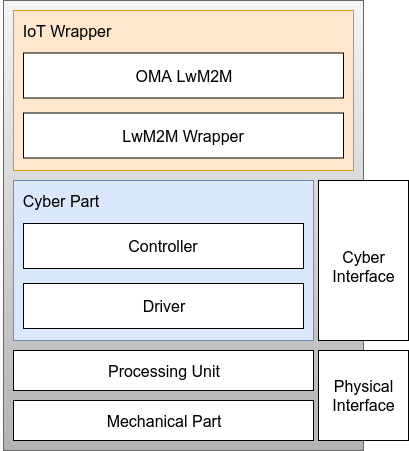
\includegraphics[height=11.5cm,width=10cm]{Figures/12.png}
	\caption{Η αρχιτεκτονική του σιλό}	
\end{figure}

	Η μεταφορά μηνυμάτων από τους drivers προς το σύστημα ελέγχου και το ανάποδο και από το δίκτυο προς το σιλό αλλά και από το σιλό προς το δίκτυο γίνεται με την χρήση Events. Στην συνέχεια θα γίνει μια εκτενέστερη αναφορά στον τρόπο που γίνεται αυτό καθ’ όλη την διάρκεια λειτουργίας του συστήματος. 
	
\section{Δομή των σιλό}

Όπως έχει ήδη αναφερθεί, στην παρούσα εργασία η ανάπτυξη του λογισμικού έγινε  βασισμένη σε συνιστώσες. Για να γίνει κάτι τέτοιο έπρεπε πρώτα να ξεχωριστούν οι διάφορες συνιστώσες από τις οποίες απαρτίζεται το σύστημα. Όπως φαίνεται και στην εικόνα 6.1 στην αρχιτεκτονική του σιλό το cyber μέρος του αποτελείται από τον driver ή τους drivers αν αυτοί είναι περισσότεροι από έναν και τον controller. Εξαιτίας αυτού έγινε η επιλογή οι διάφοροι drivers να είναι ξεχωριστά components στο σύστημα μας. Το ίδιο ισχύει και για τον controller του σιλό. Κάτι τέτοιο μας επιτρέπει να επωφεληθούμε από πολλά πλεονεκτήματα που μας δίνει τόσο αυτή η προσέγγιση όσο και το συγκεκριμένο framework (OSGi) που χρησιμοποιήσαμε, καθώς σε περίπτωση που χρειαστεί κάποια αλλαγή στο λογισμικό του συστήματος τότε αυτή μπορεί να γίνει κατά την διάρκεια που το σύστημα λειτουργεί χωρίς να επιφέρει κάποιο πρόβλημα στην λειτουργία όλου του συστήματος ελέγχου. Στις εικόνες 6.2, 6.3, 6.4, 6.5 φαίνεται η εσωτερική δομή του cyber μέρους των σιλό η οποία αποτελείται από τον controller μαζί με το state machine του που καθορίζει την συμπεριφορά του σιλό και την υποδομή των drivers του σιλό. Μέσω των διάφορων ports ο controller του σιλό επικοινωνεί με τους drivers και το περιβάλλον του.  

\begin{figure}[htbp]
	\centering
		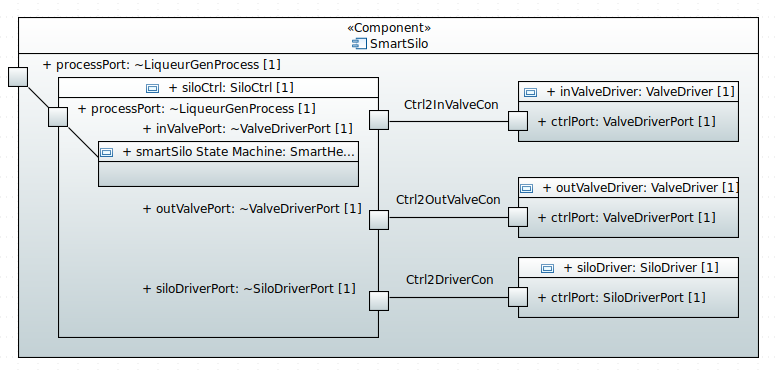
\includegraphics[height=9.5cm,width=15cm]{Figures/13.png}
	\caption{H δομή του smartSilo1}	
\end{figure}
\begin{figure}[htbp]
	\centering
		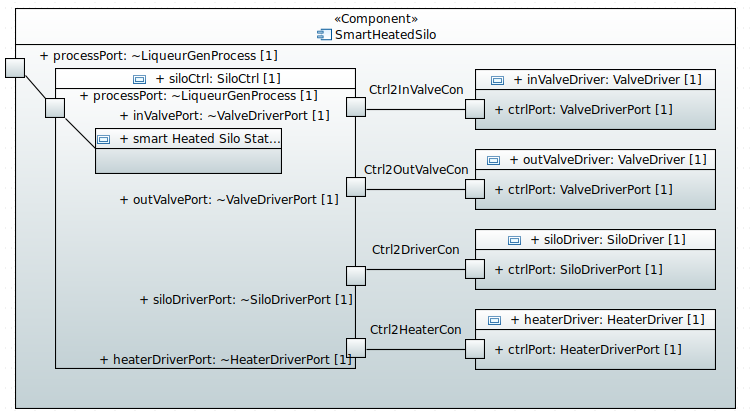
\includegraphics[height=9cm,width=15cm]{Figures/14.png}
	\caption{H δομή του smartSilo2}	
\end{figure}
\begin{figure}[htbp]
	\centering
		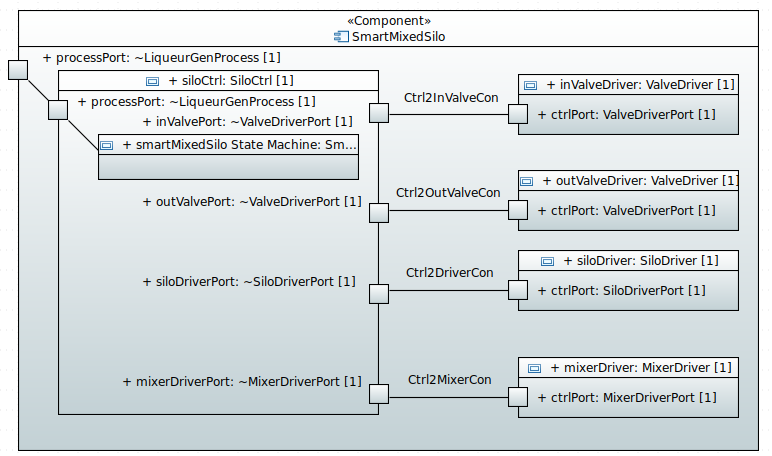
\includegraphics[height=9cm,width=15cm]{Figures/15.png}
	\caption{H δομή του smartSilo3}	
\end{figure}
\begin{figure}[htbp]
	\centering
		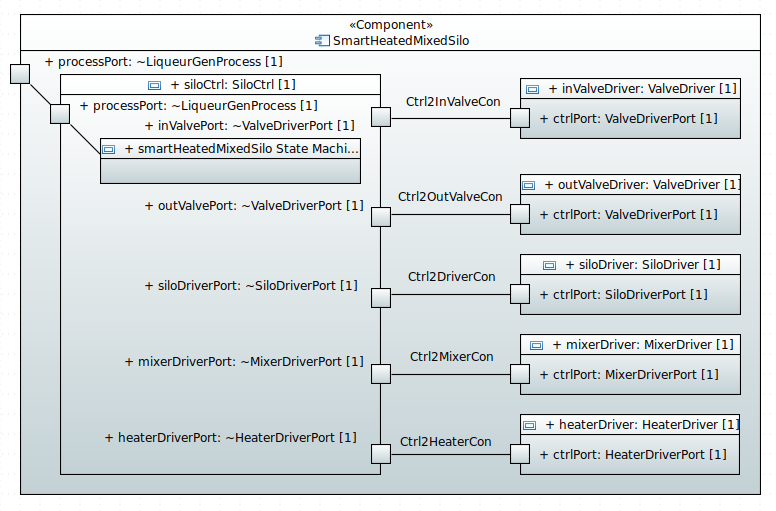
\includegraphics[height=10cm,width=15cm]{Figures/16.png}
	\caption{H δομή του smartSilo4}	
\end{figure}

\newpage

 Η δομή της συνιστώσας του controller του σιλό φαίνεται στο διάγραμμα κλάσεων της εικόνας 6.6. Η notifica-tionQueue αποτελεί την EventQueue του controller στην οποία έρχονται όλα τα μηνύματα από το περιβάλλον του σιλό. Επιπλέον μέσα από το διάγραμμα μπορούμε να ξεχωρίσουμε τις διάφορες καταστάσεις του σιλό καθώς και τον τρόπο μετάβασης από την μία μετάβαση στην άλλη μέσω των διάφορων Transitions. Παρατηρούμε επίσης ότι έχουμε ορίσει δύο κλάσεις τις State και Transition οι οποίες αποτελούν υπερκλάσεις και κληρονομούνται από τις επιμέρους καταστάσεις του σιλό και από τις μεταβάσεις από την μία κατάσταση στην άλλη αντίστοιχα. 
 
\begin{figure}[htbp]
	\centering
		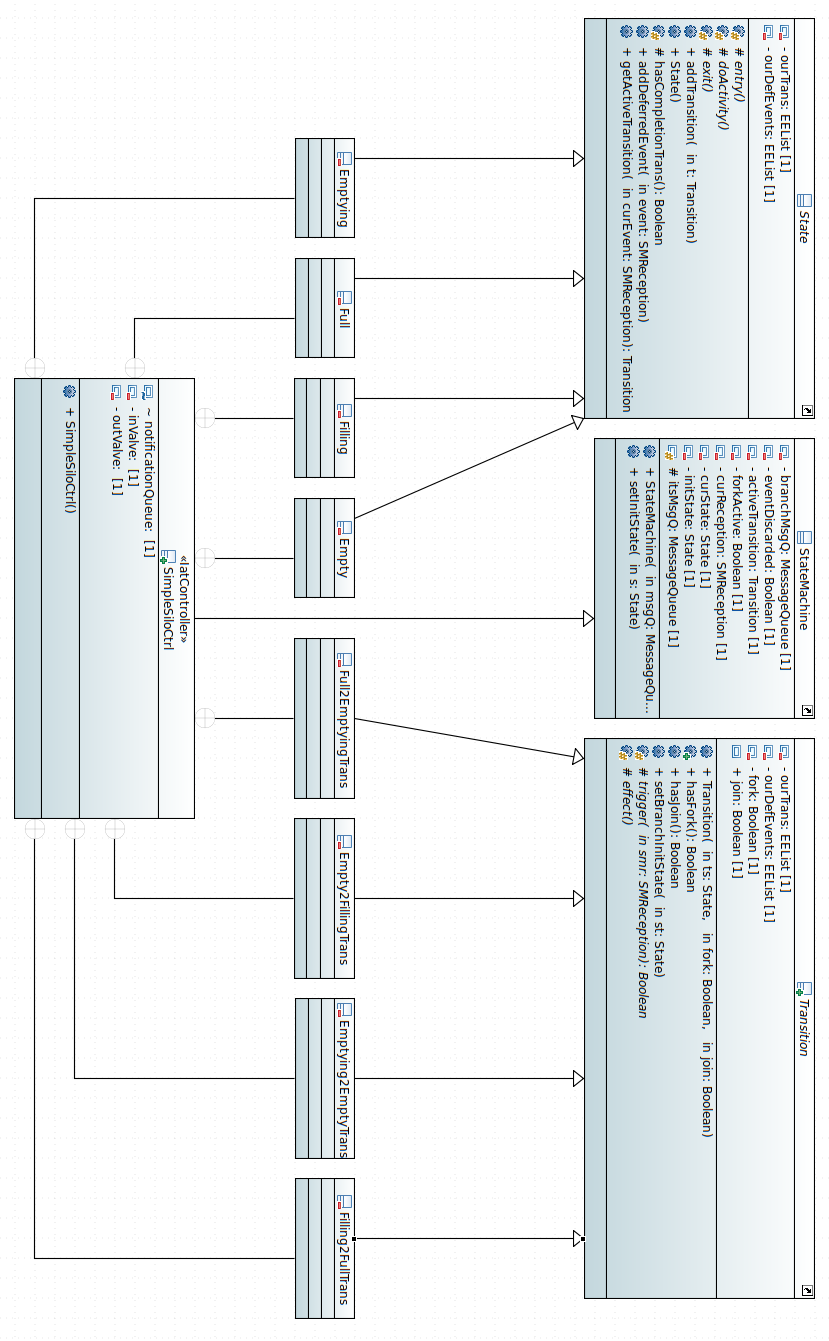
\includegraphics[height=20cm,width=14cm]{Figures/23.png}
	\caption{To διάγραμμα κλάσεων του state machine του σιλό}	
\end{figure}

\section{Συμπεριφορά του συστήματος ελέγχου}
Κάθε σιλό μπορεί να θεωρηθεί ότι κάθε στιγμή βρίσκεται σε μία συγκεκριμένη κατάσταση μέσα από ένα πεπερασμένο πλήθος καταστάσεων. Με την λήψη ενός μηνύματος είτε από τους drivers είτε από έναν LwM2M server το σιλό εκτελεί τις απαραίτητες λειτουργίες και μεταβαίνει στην επόμενη κατάσταση του. 

Ας πάρουμε για παράδειγμα, τις καταστάσεις του σιλό που περιλαμβάνει στοιχείο θέρμανσης την στιγμή που ξεκινά η λειτουργία παραγωγής liqueur τύπου Β. Αρχικά το σιλό είναι άδειο και βρίσκεται στην κατάσταση \textbf{EMPTY}. Όταν ο LwM2M client λάβει το μήνυμα Fill από τον LwM2M server τότε θα ανοίξει η πάνω βαλβίδα εισαγωγής υγρού και το σιλό θα αρχίσει να γεμίζει με liqueur και θα μεταβεί στην κατάσταση \textbf{FILLING}. Στην συνέχεια, αν ο άνω αισθητήρας ανίχνευσης υγρού ενεργοποιηθεί, δηλαδή ανιχνεύσει υγρό τότε ο driver στέλνει το μήνυμα StopFilling και το σιλό μεταβαίνει στην κατάσταση \textbf{FULL}. Ένα τέτοιο μήνυμα μπορεί να έρθει και από τον LwM2M server σε περίπτωση που κάποιος θέλει να διακόψει την εισαγωγή υγρού στο σιλό. Στην συνέχεια έρχεται από τον server ένα μήνυμα Heat και αρχίζει η λειτουργία του στοιχείου θέρμανσης του σιλό, το οποίο εισέρχεται στην κατάσταση \textbf{HEATING} μέχρις ότου φτάσει το υγρό στην επιθυμητή θερμοκρασία. Όταν γίνει αυτό ο αισθητήρας θερμοκρασίας στέλνει μέσω του driver ένα μήνυμα HeatingCompleted και το σιλό μεταβαίνει στην κατάσταση \textbf{HEATED}. Τέλος, με ένα μήνυμα Empty το σιλό μεταβαίνει στην κατάσταση \textbf{EMPTYING} και ανοίγει η βαλβίδα εξαγωγής υγρού. Μόλις το υγρό αδειάσει το σιλό μεταβαίνει στην κατάσταση \textbf{EMPTY} και η διαδικασία επαναλαμβάνεται. Αυτή η διαδικασία αναπαρίσταται από το state machine της εικόνας 6.7. Παρόμοια συμπεριφορά έχουν και τα υπόλοιπα σιλό όπως φαίνεται και στις εικόνες 6.6, 6.8, 6.9.


 Παρατηρούμε ότι όταν το σιλό βρίσκεται σε μία κατάσταση τότε πρέπει να εκτελεστεί μία λειτουργία από κάποιον driver. Όπως για παράδειγμα όταν το σιλό βρίσκεται στην κατάσταση \textbf{FILLING} ο driver πρέπει να στείλει μήνυμα στην άνω βαλβίδα ροής υγρού του σιλό ώστε αυτή να ανοίξει και όταν ο άνω αισθητήρας ανίχνευσης υγρού του σιλού ανιχνεύσει υγρό τότε η βαλβίδα πρέπει να κλείσει. Η επικοινωνία αυτή γίνεται μέσω της EventQueue του controller. Πιο αναλυτικά, όταν ο LwM2M  server που εκτελεί μια διεργασία παραγωγής liqueur ενός εκ των δύο τύπων στείλει ένα μήνυμα στον  LwM2M client του σιλό, τότε μέσω των υπηρεσίων που παρέχει η συνιστώσα του controller στο περιβάλλον της τα μηνύματα αυτά μεταφέρονται στην EventQueue του controller και από εκεί αποστέλονται τα ανάλογα μηνύματα στους drivers του σιλό μέσα από τις υπηρεσίες που η αντίστοιχη συνιστώσα του εκάστοτε driver παρέχει στο περιβάλλον της. 


\begin{figure}[htbp]
	\centering
		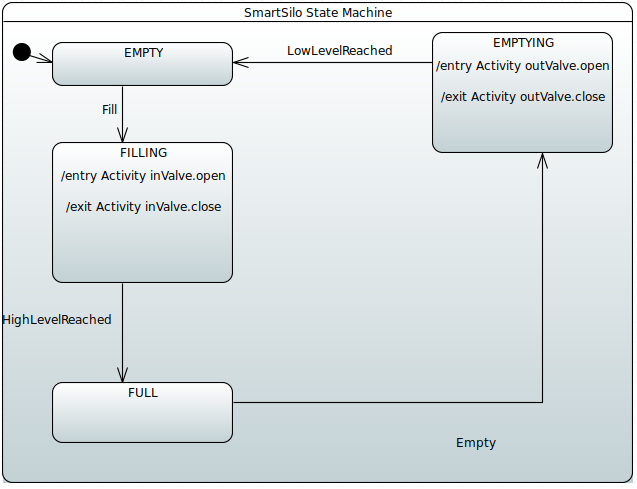
\includegraphics[height=10cm,width=15cm]{Figures/17.png}
	\caption{Το state machine του smartSilo1}	
\end{figure}
\begin{figure}[htbp]
	\centering
		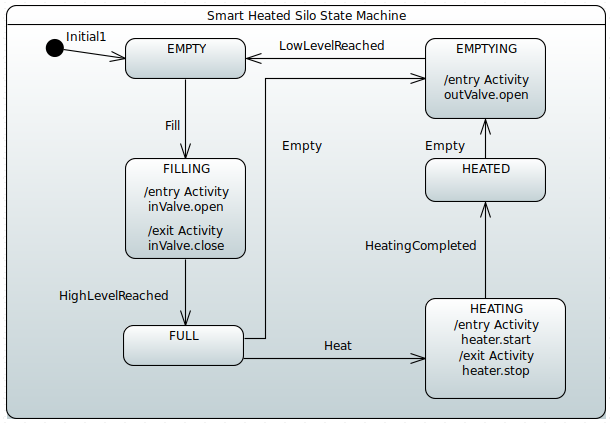
\includegraphics[height=10cm,width=15cm]{Figures/18.png}
	\caption{Το state machine του smartSilo2}	
\end{figure}
\begin{figure}[htbp]
	\centering
		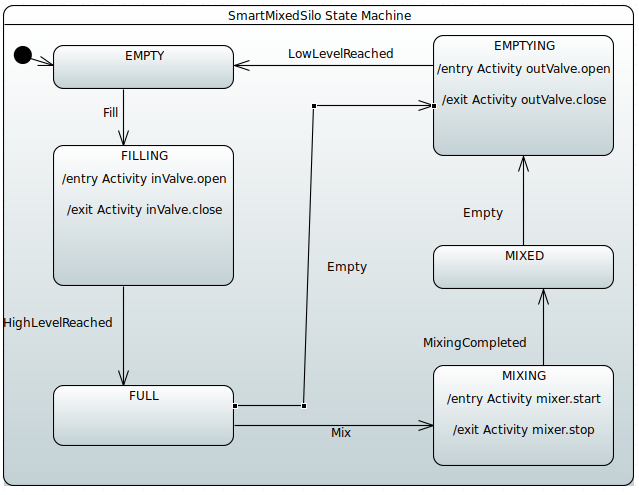
\includegraphics[height=10cm,width=15cm]{Figures/19.png}
	\caption{Το state machine του smartSilo3}	
\end{figure}
\begin{figure}[htbp]
	\centering
		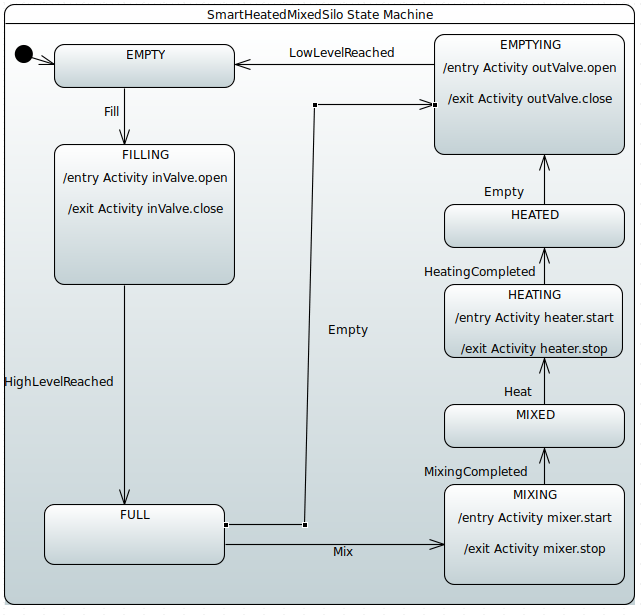
\includegraphics[height=12cm,width=15cm]{Figures/20.png}
	\caption{Το state machine του smartSilo4}	
\end{figure}





\addtocontents{toc}{\vspace{2em}}
\chapter{Υλοποίηση του συστήματος} % Main chapter title

\label{Chapter7} 

\section{Γενικά}
 Σε αυτή την ενότητα θα γίνει μία εκτενής περιγραφή στην ανάπτυξη του συστήματος ελέγχου του σιλό σύμφωνα με τις προδιαγραφές που αναφέρθηκαν παραπάνω. Η υλοποίηση του συστήματος ελέγχου έγινε σε Java χρησιμοποιώντας την component-based προσέγγιση για την ανάπτυξη του λογισμικού. Χρησιμοποιήθηκε το OSGi framework καθώς παρείχε αρκετά πλεονεκτήματα και αρκετές υπηρεσίες που κρίθηκαν πολύ βοηθητικές. Επιπλέον, χρησιμοποιώντας Java για την ανάπτυξη του συστήματος ελέγχου έχουμε αρκετές επιλογές για το υλικό που μπορεί να χρησιμοποιηθεί καθώς η συγκεκριμένη γλώσσα μπορεί να τρέξει σε μεγάλο εύρος συσκευών. Επιπλέον, επιλέγοντας την συγκεκριμένη γλώσσα προγραμματισμού δίνεται η δυνατότητα χρήσης δύο βιβλιοθηκών που υλοποιούν τα πρωτόκολλα CoAP και LwM2M, τις Californium και Leshan αντίστοιχα, καθώς και της βιβλιοθήκης pi4j [60] που μας επιτρέπει να χρησιμοποιήσουμε τα γενικού σκοπού I/O του Raspberry Pi μέσω της Java. 

	Στην συγκεκριμένη εργασία χρησιμοποιήθηκαν σαν ενσωματωμένοι μικροϋπολογιστές  Raspberry Pi 3 Model B και Raspberry Pi 2 Model B.  Η υλοποίηση του συστήματος ελέγχου έγινε στο Intellij IDEA IDE της Jetbrains καθώς υπήρχε άδεια για την χρησιμοποίηση της έκδοσης  Ultimate μέσω του Πανεπιστημίου. Tέλος χρησιμοποιήθηκε το σύστημα ελέγχου πηγαίου κώδικα Git σε συνδυασμό με την υπηρεσία Github. 
	
\section{Οι συνιστώσες του συστήματος ελέγχου}
Όπως έχει ήδη αναφερθεί, η υλοποίηση του λογισμικού του συστήματος έγινε χρησιμοποιώντας την προσέγγιση συνιστωσών με την βοήθεια του OSGi framework. Για να γίνει κάτι τέτοιο έπρεπε αρχικά να ξεχωριστούν οι διάφορες συνιστώσες του συστήματος. Φυσικά και το σύστημα ελέγχου θα μπορούσε να υλοποιηθεί σε ένα μόνο component. Κάτι τέτοιο όμως θα σήμαινε ότι το σύστημα ελέγχου θα υλοποιούνταν σαν ένα Plain Old Java Object (POJO) και ως συνέπεια δεν θα μπορούσαμε να επωφεληθούμε από τα πλεονεκτήματα που μας προσφέρει το OSGi. Κατά συνέπεια αποφασίστηκε το σύστημα ελέγχου να αποτελείται από πολλές συνιστώσες, όπου κάθε μία θα είναι υπεύθυνη για μία λειτουργία του σιλό. Στην εικόνα 7.1 φαίνονται οι συνιστώσες από τις οποίες αποτελείται το σύστημα. Το διάγραμμα αυτό είναι ένα component διάγραμμα όπως το προτείνει η OSGi Alliance [48] και δείχνει τη δομή του cyber μερους του σιλό ως Industrial Automation Thing. Κάθε συνιστώσα σε αυτό το διάγραμμα αντιστοιχεί σε ένα φυσικό μέρος του σιλό το οποίο μπορεί να αντικατασταθεί ανά πάσα στιγμή. 

	Ένα πολύ σημαντικό χαρακτηριστικό του OSGi είναι ότι οι διάφορες συνιστώσες του συστήματος θα πρέπει να επικοινωνούν μεταξύ τους μέσω καλά καθορισμένων interfaces. Έτσι κάθε συνιστώσα πρέπει να εξάγει τις διεπαφές που είναι απαραίτητες ώστε να επικοινωνήσει με το περιβάλλον της και κάποια άλλη συνιστώσα να μπορεί να επικοινωνήσει με αυτή. Στο διάγραμμα μπορούμε να παρατηρήσουμε ότι κάθε .api συνιστώσα εξάγει το πακέτο που περιέχει τα διάφορα interfaces της. Το πακέτο που εξάγεται εμφανίζεται στο διάγραμμα σαν ένα μαύρο κουτί μέσα στο component, ενώ τα πακέτα που το  κάθε component απαιτεί ώστε να μπορέσει να λειτουργήσει μοντελοποιούνται σαν λευκά κουτιά. Για παράδειγμα, η συνιστώσα valve.out υλοποιεί την λειτουργικότητα του driver της βαλβίδας εξαγωγής υγρού του σιλό και η συνιστώσα valve.out.api καθορίζει τις υπηρεσίες που παρέχει η βαλβίδα εξαγωγής υγρού στον περιβάλλον της. Ο controller του σιλό στην εικόνα 7.1 πρέπει να χρησιμοποιήσει τις .api συνιστώσες των τριών drivers, δηλαδή του siloDriver που είναι υπεύθυνος για την λειτουργικότητα των αισθητήρων,  του inValveDriver  και του outValveDriver που είναι υπεύθυνοι για την λειτουργικότητα της βαλβίδας εισαγωγής και εξαγωγής υγρού αντίστοιχα. Στη συνέχεια θα γίνει μία εκτενέστερη ανάλυση του τρόπου λειτουργίας της κάθε συνιστώσας καθώς και του τρόπου χρήσης του OSGi.
	
\begin{figure}[htbp]
	\centering
		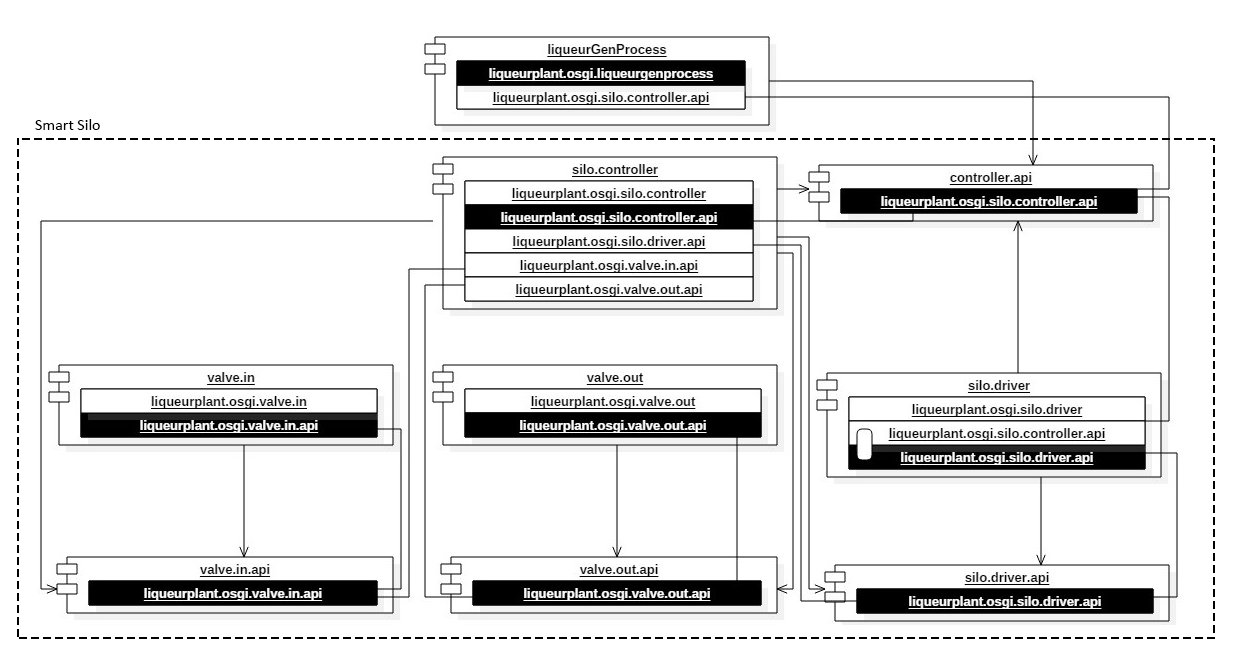
\includegraphics[height=10cm,width=16cm]{Figures/21.png}
	\caption{Το διάγραμμα συνιστωσών ενός σιλό}	
\end{figure}

\section{Ανάλυση των συνιστωσών του συστήματος ελέγχου}

\subsection{Οι συνιστώσες των drivers του σιλό}
Όπως περιγράφηκε και στην προηγούμενη ενότητα, κάθε συνιστώσα είναι υπεύθυνη για την λειτουργικότητα ενός φυσικού στοιχείου του σιλό. Αυτό σημαίνει ότι για κάθε στοιχείο που εκτελεί ένα έργο για το σύστημα θα υπάρχει ένα component υπεύθυνο για την υλοποίηση και ένα component υπεύθυνο για τις υπηρεσίες που εξάγει στο περιβάλλον του. Έτσι έχουμε την ακόλουθη αντιστοίχηση φυσικών μερών του συστήματος με συνιστώσες λογισμικού που φαίνεται στον πίνακα 7.1:


\begin{table}[h]
\centering
\begin{tabular}{|c|c|}
\hline
\textbf{Φυσικό Μέρος του Σιλό} & \textbf{Component λογισμικού} \\ \hline
Βαλβίδα εισαγωγής υγρού & Valve.in \\ \hline
Βαλβίδα εξαγωγής υγρού & Valve.out \\ \hline
Στοιχείο ανάδευσης του υγρού & Mixer.driver \\ \hline
Στοιχείο θέρμανσης του υγρού & Heater.driver \\ \hline
Αισθητήρες επιπέδου υγρού & Silo.driver \\ \hline
\end{tabular}
\caption{Αντιστοίχηση των φυσικών μερών του σιλό με τη συνιστώσα τους}
\label{my-label}
\end{table}

\subsubsection{Συνιστώσες βαλβίδων του σιλό}
	Είναι υπεύθυνες για την αντιστοίχηση του μηχανικού μέρους της βαλβίδας του σιλό σε επίπεδου λογισμικού ώστε να μπορεί να χρησιμοποιηθεί από τον ενσωματωμένο μικροϋπολογιστή και να παρέχει τις υπηρεσίες που περιγράφηκαν στο κεφάλαιο 6 στο περιβάλλον του. Γι’ αυτό οι συγκεκριμένες συνιστώσες αποτελούνται από μία διεπαφή (.api component) μέσω τις οποίας παρέχουν στον περιβάλλον τους υπηρεσίες για το άνοιγμα και το κλείσιμο της βαλβίδας. Αυτές οι διεπαφές υλοποιούνται από τα components valve.in και valve.out όπου με την βοήθεια της βιβλιοθήκης pi4j αποστέλνεται σήμα στην βαλβίδα να ανοίξει ή να κλείσει ανάλογα με την περίπτωση.  Η διεπαφή των βαλβίδων αποτελείται από το interface ValveDriverIf το οποίο ορίζει τις μεθόδους open() και close() οι οποίες ανοίγουν και κλείνουν την βαλβίδα αντίστοιχα. Στο component που υλοποιεί αυτή τη λειτουργικότητα έχουμε την υλοποίηση αυτών των μεθόδων, όπου κάθε μέθοδος αλλάζει την τάση σε ένα συγκεκριμένο γενικού σκοπού I/O του Raspberry Pi. Αξίζει επίσης να σημειωθεί ότι χρησιμοποιήθηκαν και όροι OSGi ώστε να μπορεί αυτή η υλοποίηση να είναι component. Αυτό γίνεται χρησιμοποιώντας το annotation \textbf{@Component} μέσα στο οποίο ορίζεται το όνομα της συνιστώσας καθώς και το όνομα της υπηρεσίας που απαιτεί για να λειτουργήσει. Αυτά φαίνονται καλύτερα και στον αλγόριθμο 7.1 όπου βλέπουμε την υλοποίηση του component για την βαλβίδα εξαγωγής υγρού από το σιλό. 

\newpage

\begin{lstlisting}[caption=Μέρος της υλοποίησης της συνιστώσας την βαλβίδας εξαγωγής υγρού]
$$@Component(
        name = "liqueurplant.osgi.valve.out",
        service = liqueurplant.osgi.valve.out.api.OutValveDriverIf.class
)
public class OutValveDriver implements OutValveDriverIf {
	.
	.
	.
    $$@Override
    public void open() throws Exception {
        try {
            outValvePin.setState(PinState.LOW);
        } catch (Exception e) {
            LOGGER.error("Exception in open(): " + e.toString());
        }
    }

    $$@Override
    public void close() throws Exception {
        try {
            outValvePin.setState(PinState.HIGH);
        } catch (Exception e) {
            LOGGER.error("Exception in close(): " + e.toString());
        }
    }
}
\end{lstlisting}

\subsubsection{Συνιστώσες στοιχείων θέρμανσης και μίξης του σιλό}
Είναι υπεύθυνες για την λειτουργικότητα των στοιχείων ανάδευσης και θέρμανσης του υγρού που μπορεί να περιέχει κάποιο σιλό. Σχετικά με το στοιχείο ανάδευσης του υγρού, αποτελείται από ένα .api component μέσω του οποίου παρέχει τις υπηρεσίες έναρξης και τερματισμού λειτουργίας του μηχανικού μέρους για την ανάδευση του υγρού. Αυτές οι υπηρεσίες παρέχονται μέσω ενός interface στον περιβάλλον του σιλό, το MixerDriverIf και υλοποιούνται από το mixer component στο οποίο όταν έρθει εντολή για έναρξη ανάδευσης το υγρό αναμειγνύεται για συγκεκριμένο χρόνο και η διαδικασία αυτή σταματάει όταν έρθει εντολή τερματισμού. Πάλι και εδώ χρησιμοποιούνται τα αντίστοιχα annotations ώστε το περιβάλλον του OSGi να μπορεί να αναγνωρίζει τη συγκεκριμένη συνιστώσα σαν component. Για το στοιχείο θέρμανσης ακολουθήθηκε παρόμοια λογική, πέρα από το γεγονός ότι υλοποιήθηκε και ένα callback καθώς ήταν απαραίτητη η εισαγωγή πληροφορίας από το μηχανικό μέρος του σιλό. Έτσι μόλις ο αισθητήρας θερμοκρασίας του σιλό επιστρέψει την επιθυμητή τιμή καλείται η μέθοδος heatingCompleted ώστε να σταματήσει η διαδικασία θέρμανσης του υγρού. Στον αλγόριθμο 7.2 φαίνονται οι υπηρεσίες που παρέχει η συνιστώσα του στοιχείου θέρμασης του σιλό στον περιβάλλον της. 


\begin{lstlisting}[caption=Οι υπηρεσίες που παρέχει η συνιστώσα του στοιχείου θέρμανσης]
$$@ProviderType
public interface HeaterDriverIf {
    void start();
    void stop();
    void heat2temp(float temperature);
    void addHeatingCompletedListener(HeatingCompletedListenerIf listener);
}

\end{lstlisting}

Με τη χρήση του annotation \textbf{@ProviderType} οι υπηρεσίες αυτές εγγράφονται στο μητρώο υπηρεσίων του OSGi και μπορούν να χρησιμοποιηθούν από άλλες συνιστώσες.


\subsubsection{Συνιστώσα του driver του σιλό}
Ο συγκεκριμένος driver είναι υπεύθυνος για τους αισθητήρες επιπέδου του υγρού. Η συγκεκριιμένη συνιστώσα δεν συνοδεύεται από ένα component .api καθώς δεν μπορεί να εξάγει κάποια υπηρεσία. Αυτό έγινε γιατί αντιμετωπίστηκε το πρόβλημα των κυκλικών εξαρτήσεων μεταξύ του συστήματος ελέγχου και της συνιστώσας του driver του σιλό. Γι’ αυτό το λόγο ακολουθήθηκε μία διαφορετική προσέγγιση κατά την οποία ο driver επικοινωνεί με τον controller μέσω της EventQueue του controller. Για να γίνει αυτό πιο σαφές, ας θεωρήσουμε ότι το σιλό βρίσκεται στην κατάσταση FILLING. Όταν το υγρό φτάσει στο ανώτατο σημείο του σιλό τότε ο άνω αισθητήρας ανίχνευσης υγρού θα ενεργοποιηθεί και ο driver θα εισάγει στην EventQueue του controller ένα μήνυμα ότι το σιλό έχει γεμίσει ώστε το σύστημα ελέγχου να συνεχίσει τις απαραίτητες διαδικασίες ώστε να λειτουργήσει σωστά όλο το σύστημα παραγωγής. Κάτι τέτοιο δημιουργεί την ανάγκη η συνιστώσα του driver να χρειάζεται τις υπηρεσίες που παρέχει η συνιστώσα του controller για να λειτουργήσει. Αυτό φαίνεται και από το reference που υπάρχει στην συνιστώσα του controller στην υλοποίηση του driver που φαίνεται στον αλγόριθμο 7.3. 
\begin{lstlisting}[caption=Μέρος της υλοποίησης της συνιστώσας του driver του σιλό]

$$@Component(
        name = "liqueurplant.osgi.silo.driver",
        immediate = true
)
public class SimpleSiloDriver {
   .
   .
   .
    $$@Reference(
            policy = ReferencePolicy.DYNAMIC,
            cardinality = ReferenceCardinality.OPTIONAL
    )
    protected void setSiloCtrlIf(SiloCtrlIf siloCtrl) {
        this.siloCtrl = siloCtrl;
        LOGGER.info("SILO-CONTROLLER binded.");
    }

    protected void unsetSiloCtrlIf(SiloCtrlIf siloCtrl) {
        this.siloCtrl = null;
        LOGGER.info("SILO-CONTROLLER unbinded.");
    }
}
\end{lstlisting}

Από μερίας λογισμικού, ο driver του σιλό υλοποιεί δύο \textbf{Listeners} με την βοήθεια της βιβλιοθήκης Pi4j, και συγκεκριμένα του interface GpioPinListenerDigital. Ο listener που αφορά την ακίδα που είναι υπεύθυνη για τον άνω αισθητήρα παρουσίας υγρού του σιλό περιμένει να λάβει σήμα υψηλής τάσης στο γενικού σκοπού I/O του Raspberry Pi από τον εξομοιωτή του σιλό. Όταν έρθει το συγκεκριμένο σήμα τότε εισάγει στην EventQueue του σιλό ένα νέο Signal ότι το υγρό έχει γεμίσει το σιλό. Ομοίως υπάρχει και ένας Listener για  τον κάτω αισθητήρα παρουσίας υγρού του σιλό. Η υλοποίηση αυτή φαίνεται και στον αλγόριθμο 7.4. Αξίζει να σημειωθεί ότι το annotation \textbf{@Activate} που υπάρχει στο πάνω μέρος της μεθόδου, αποτελεί μέρος του OSGi framework και αφορά τον κύκλο ζωής της συγκεκριμένης συνιστώσας. Έτσι μόλις ενεργοποιηθεί η συγκεκριμένη συνιστώσα θα τρέξει η μέθοδος αυτή ώστε να γίνουν οι απαραίτητες αρχικοποιήσεις.
\newpage
\begin{lstlisting}[caption=Η υλοποίση των listener του driver του σιλό]
$$@Activate
public void activate() {
	highLevelSensorPin = gpioController.provisionDigitalInputPin(RaspiPin.GPIO_02, "HIGH-LEVEL-SENSOR", PinPullResistance.PULL_DOWN);
	lowLevelSensorPin = gpioController.provisionDigitalInputPin(RaspiPin.GPIO_03, "LOW-LEVEL-SENSOR", PinPullResistance.PULL_DOWN);

	highLevelSensorPin.setShutdownOptions(true);
	lowLevelSensorPin.setShutdownOptions(true);

	highLevelSensorPin.addListener((GpioPinListenerDigital) event -> {
		if (event.getState() == PinState.HIGH) {
			siloCtrl.put2MsgQueue(new HighLevelReachedSignal());
		}
	});
	lowLevelSensorPin.addListener((GpioPinListenerDigital) event -> {
		if (event.getState() == PinState.LOW) {
			siloCtrl.put2MsgQueue(new LowLevelReachedSignal());
		}
	});
}
\end{lstlisting}

\subsubsection{Συνιστώσα του controller του σιλό}
Αποτελεί το βασικό μέρος του συστήματος ελέγχου, καθώς όλα τα μηνύματα που έρχονται τόσο από τον LwM2M server όσο και από τους drivers του σιλό πρέπει να επεξεργαστούν από τον συγκεκριμένο μέρος του συστήματος. Η συγκεκριμένη συνιστώσα του συστήματος περιλαμβάνει μία EventQueue μέσα στην οποία μπορούν να τοποθετηθούν διάφορα μηνύματα που αφορούν τη λειτουργία του σιλό. Ένα άλλο σημαντικό κομμάτι της υλοποίησης είναι το Generic State Machine που χρησιμοποιήθηκε στον controller του σιλό. 

Αυτό το state machine έχει υλοποιηθεί σε άλλη διπλωματική εργασία που έγινε παράλληλα με την εκπόνηση της παρούσας και χρησιμοποιείται στο controller του σιλό ώστε να γίνεται η επεξεργασία των μηνυμάτων που λαμβάνει καθώς και οι κατάλληλες ενέργειες που απαιτούνται ώστε να επιτευχθεί σωστή λειτουργία του συστήματος ελέγχου. Έχει υλοποιηθεί με μοντέλο την μηχανή καταστάσεων της UML. Αυτό σημαίνει ότι πρέπει να δηλωθούν οι διαφορετικές καταστάσεις στις οποίες μπορεί να βρεθεί το σιλό καθώς και οι διάφορες μεταβάσεις από την μία κατάσταση στην άλλη. Κάθε κατάσταση περιέχει τρεις μεθόδους τις entry, doActivity, exit όπως ακριβώς ορίζει και η UML. Σε αυτές τις μεθόδους εκτελούνται ενέργειες όταν το σιλό εισέλθει σε μία νέα κατάσταση, κατά την διάρκεια που βρίσκεται σε αυτή και πριν μεταβεί σε κάποια επόμενη κατάσταση αντίστοιχα. Σε αυτές τις μεθόδους βρίσκεται το μεγαλύτερο μέρος της λογικής του συστήματος ελέγχου. 

	
	Ο controller του συστήματος παρέχει μέσω της .api συνιστώσας υπηρεσίες υπεύθυνες για την εισαγωγή και εξαγωγή μηνυμάτων από την EventQueue του, οι οποίες φαίνονται στον αλγόριθμο 7.5. Αξίζει να σημειωθεί ότι η EventQueue υλοποιήθηκε με την χρήση της τεχνολογίας ArrayBlockingQueue που μας παρείχε η Java καθώς θα έπρεπε να χρησιμοποιείται από δύο νήματα που θα τρέχουν ταυτόχρονα. Κάτι τέτοιο μας έδωσε την δυνατότητα να μην πέσουμε σε κάποιο deadlock και τα νήματα τόσο του controller όσο και του LwM2M client να λειτουργούν χωρίς να παρουσιαστεί κάποιο πρόβλημα. 

	Η συγκεκριμένη συνιστώσα πρέπει ανάλογα με τον τύπο του σιλό να περιμένει να λάβει τις υπηρεσίες από τα διάφορα άλλα components όπως για παράδειγμα των βαλβίδων και του driver του σιλό. 
	
\begin{lstlisting}[caption=Οι υπηρεσίες που παρέχει η συνιστώσα του ελεγκτή του σιλό]
$$@ProviderType
public interface SiloCtrlIf {
    void put2MsgQueue(BaseSignal signal);
    BaseSignal takeNotification();
}

\end{lstlisting}


\subsubsection{Ο LwM2M client του σιλό}
Η συνιστώσα που υλοποιεί τον LwM2M  client του συστήματος ελέγχου είναι υπεύθυνη για την επικοινωνία του σιλό με το εξωτερικό του περιβάλλον. Δημιουργεί κάποια από τα objects και τα resources που αναλύθηκαν στο κεφάλαιο 6 και τα καθιστά προσβάσιμα μέσω του πρωτοκόλλου CoAP ώστε να μπορούν να χρησιμοποιηθούν από έναν LwM2M server. Μόλις ξεκινήσει η λειτουργία του συστήματος η συγκεκριμένη συνιστώσα είναι υπεύθυνη για να κάνει εγγραφή σε έναν LwM2M server, του οποίου γνωρίζει την IP του. Όταν γίνει αυτή η εγγραφή τότε ενημερώνει τον server για τα object και τα resources που παρέχει ο συγκεκριμένος client. Επιπλέον, είναι σημαντικό να σημειωθεί ότι ο client περιμένει να λάβει τις υπηρεσίες του controller ώστε να μπορέσουν να μεταφερθούν τα διάφορα μηνύματα που θα λάβει από τον server και το σύστημα να λειτουργήσει σωστά. 

\newpage
\section{Η πειραματική διάταξη}
Για να ελεγχθεί η σωστή λειτουργία του συστήματος ελέγχου που υλοποιήθηκε ήταν αναγκαία μία προσομοίωση της διαδικασίας παραγωγής liqueur. Για να γίνει αυτό όπως προαναφέρθηκε χρησιμοποιήθηκαν Raspberry Pi σαν ενσωματωμένοι μικροϋπολογιστές πάνω στους οποίους έτρεχε και το σύστημα ελέγχου. Επίσης, χρησιμοποιήθηκε και ένας προσομοιωτής του μηχανικού σιλό που είχε υλοποιηθεί στην [61]. Ο προσομοιωτής του μηχανικού σιλό όπως φαίνεται στην εικόνα 7.4 αποτελείται από ένα ψηφιακό ηλεκτρονικό κύκλωμα και επικοινωνεί με τον μικροϋπολογιστή Raspberry Pi με την αποστολή ψηφιακών ηλεκτρικών σημάτων.

	
\begin{figure}[htbp]
	\centering
		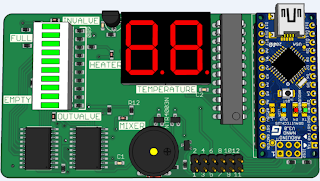
\includegraphics[height=5.5cm,width=10cm]{Figures/24.png}
	\caption{Εξομοιωτής των μηχανικών στοιχείων του σιλό \cite{Foivos}}	
\end{figure}

Το κύκλωμα διαθέτει, σύμφωνα με την [61]:
\begin{itemize}
	\item{μία μπάρα LED 10 τμημάτων για την απεικόνιση της στάθμης του υγρού ανά πάσα στιγμή μέσα στο σιλό}
	\item{δύο LED για την ένδειξη της κατάστασης των βαλβίδων εισόδου και εξόδου}
	\item{δύο LED για την ένδειξη των αισθητήρων παρουσίας υγρού}
	\item{ένα LED για την ένδειξη της κατάστασης του στοιχείου θέρμανσης και ένα LED αλλά και ένα buzzer για την ένδειξη της κατάστασης του στοιχείου μίξης}
	\item{δύο 7-segment displays για την ένδειξη της τρέχουσας θερμοκρασίας του σιλό. }
\end{itemize}

Για την επικοινωνία με τον μικροϋπολογιστή που χρησιμοποιήθηκε, χρησιμοποιήθηκαν οι διεπαφές που είχε ο εξομοιωτής του μηχανικού σιλό οι οποίες ήταν καλά ορισμένες μέσω της [61]. Από το Raspberry Pi αποστέλλονται ψηφιακά σήματα μέσω της βιβλιοθήκης Pi4J και τα γενικού σκοπού Ι/Ο που παρέχει το Raspberry Pi. 

	Είχαμε στην διάθεση μας τέσσερις εξομοιωτές του σιλό και έναν εξομοιωτή του Pipe που φαίνεται στην εικόνα 7.5. Έτσι αφού εγκαταστάθηκε το Apache Felix Framework στους μικροϋπολογιστές και έγιναν οι κατάλληλες διασυνδέσεις με τους εξομοιωτές των μηχανικών τμημάτων του σιλό το σύστημα ήταν έτοιμο για χρήση. Για την διεξαγωγή των πειραμάτων χρησιμοποιήθηκε ένα LwM2M server ο οποίος υλοποιούσε την λογική της παραγωγής και των δύο τύπων liqueur ταυτόχρονα. Ο LwM2M server είναι υλοποιημένος σε Java σαν ένα POJO και έτρεχε σε ένα Raspberry Pi 2 Model B, το οποίο απαρτίζεται από έναν τετραπύρηνο επεξεργαστή χρονισμένο στα 900MHz και από 1 Gb RAM. Η διαδικασία για την παραγωγή του liqueur τύπου Β φαίνεται στην εικόνα 7.6.
	
\begin{figure}[htbp]
	\centering
		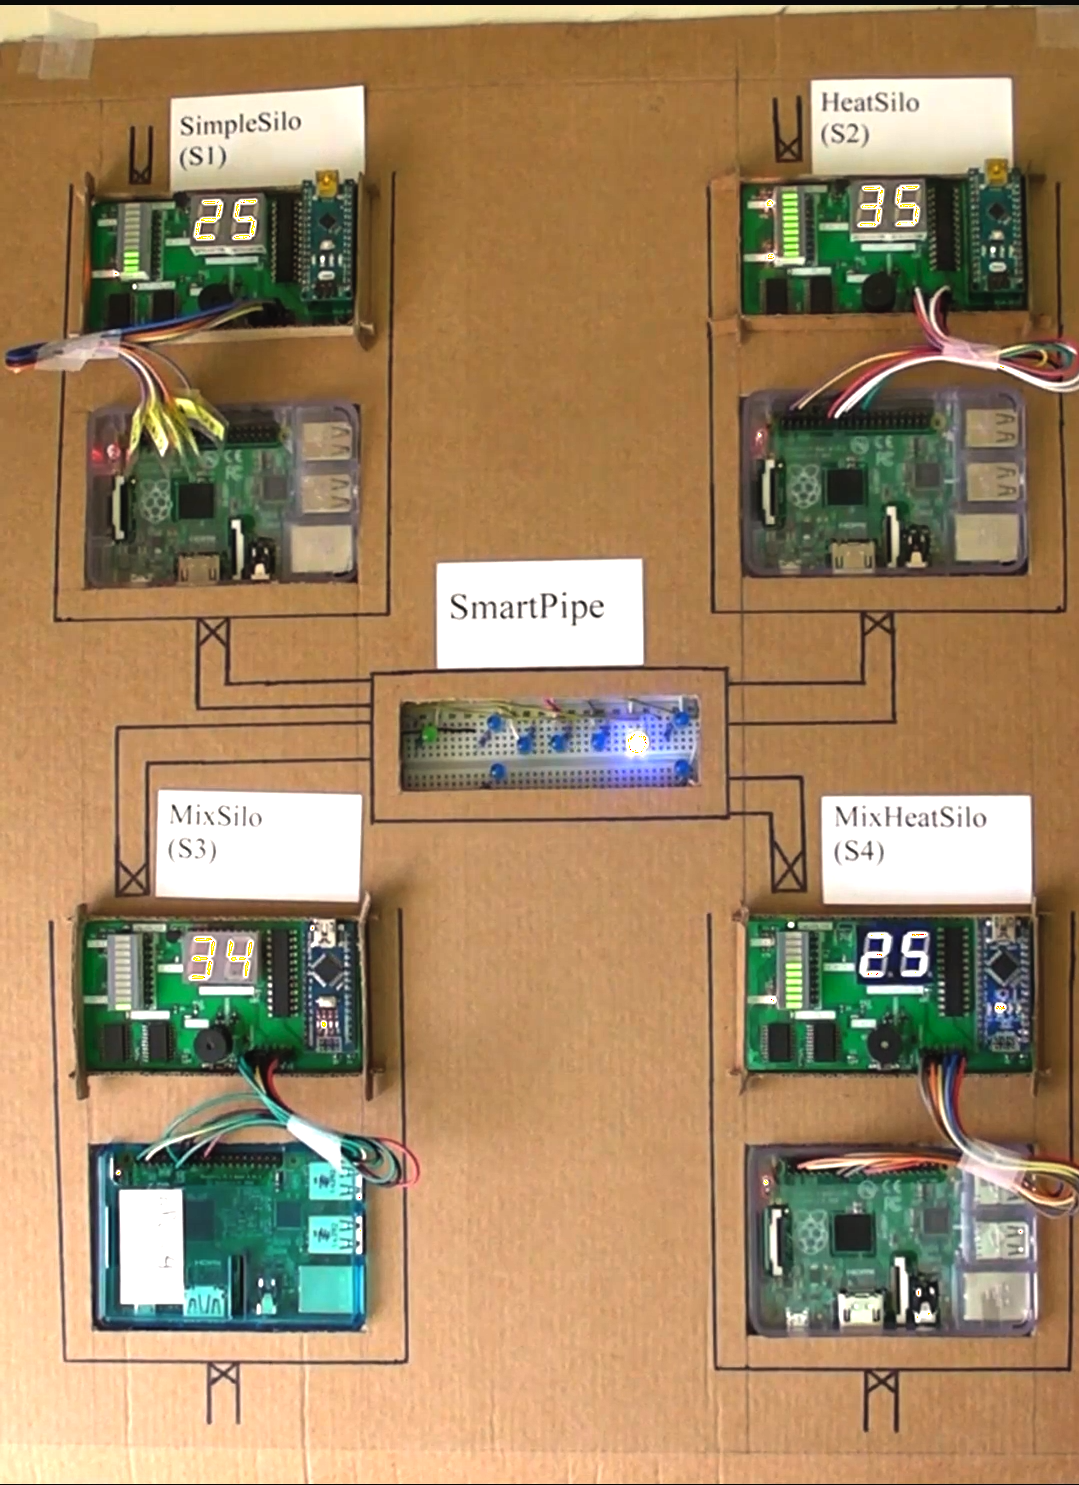
\includegraphics[height=14cm,width=10cm]{Figures/25.png}
	\caption{H πειραματική διάταξη με τα τέσσερα σιλό και τον σωλήνα}	
\end{figure}

\begin{figure}[htbp]
	\centering
		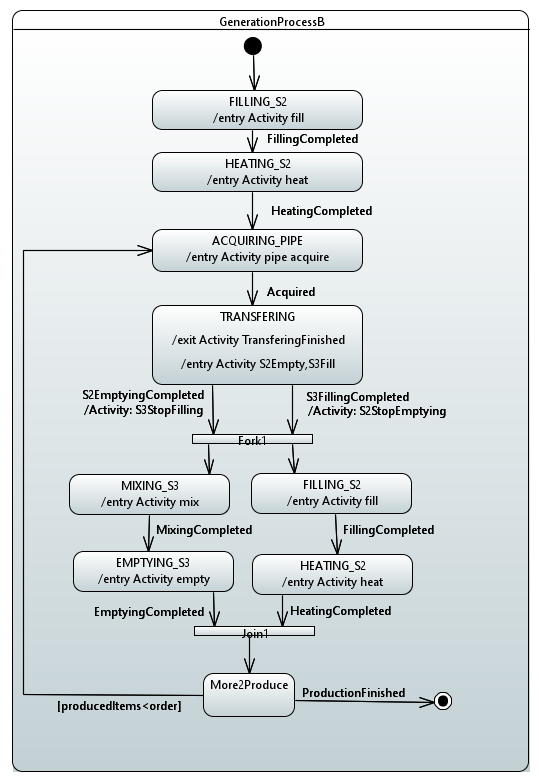
\includegraphics[height=20cm,width=14cm]{Figures/26.PNG}
	\caption{Η διαδικασία παραγωγής liqueur τύπου Β}	
\end{figure}
\addtocontents{toc}{\vspace{2em}}
\chapter{ Συμπεράσματα και μελλοντική εργασία} % Main chapter title

\label{Chapter8}

 

\noindent Στην εργασία αυτή περιγράφεται ο σχεδιασμός και η ανάπτυξη ενός συστήματος ελέγχου για ένα βιομηχανικό σύστημα παραγωγής χρησιμοποιώντας μία προσέγγιση συνιστωσών καθώς και τεχνολογίες διαδικτύου, ώστε να μετατραπεί το παραδοσιακό βιομηχανικό σύστημα σε ένα σύστημα συμβατό με το διαδίκτυο των αντικειμένων. Η επικοινωνία των επιμέρους υποσυστημάτων έγινε με την χρήση του LwM2M που ακολουθεί της αρχές τις REST αρχιτεκτονικής και η ανάπτυξη του συστήματος ελέγχου βασίστηκε στην ανάπτυξη λογισμικού με την προσέγγιση συνιστωσών. 

\section{Συμπεράσματα}
Μέσω της εργασίας αυτής μου δόθηκε η δυνατότητα να μελετήσω αρχικά εις βάθος την προσέγγιση ανάπτυξης λογισμικού με συνιστώσες και κυρίως το framework OSGi που παρέχει αυτή τη δυνατότητα στην γλώσσα προγραμματισμού Java. Μέσω αυτής της μελέτης απέκτησα σπουδαία γνώση στον τρόπο με τον οποίο μπορεί να δομηθεί ένα πρόγραμμα ακολουθώντας την συγκεκριμένη προσέγγιση, αφού σε πολλά σημεία χρειάστηκε να ανατρέξω σε πηγαίο κώδικα προκειμένου να συλλεχθούν οι απαραίτητες πληροφορίες που χρειάστηκαν στα πλαίσια της εργασίας μου. Επιπλέον, η ομάδα που είναι υπεύθυνη για το συγκεκριμένο framework έχει κάνει άριστη δουλειά στο documentantion το οποίο ήταν σύμμαχος μου σε οποιοδήποτε πρόβλημα κλήθηκα να αντιμετωπίσω. Επιπλέον, ήρθα σε επαφή με την γλώσσα μοντελοποίησης UML, την οποία σε συνεργασία με τον επιβλέποντα καθηγητή της εργασίας κατανόησα εις βάθος ώστε να μπορέσω να σχεδιάσω το σύστημα που ανέπτυξα με τον καλύτερο δυνατό τρόπο. Ο σχεδιασμός του συστήματος με την χρήση της γλώσσας UML ήταν ίσως το σημαντικότερο μέρος της εργασίας καθώς από την στιγμή που καταλήξαμε σε μερικές παραδοχές τότε η ανάπτυξη του συστήματος ακολουθώντας τις προδιαγραφές που ορίστηκαν ήταν αρκετά δομημένη και απλή. Επίσης, ήρθα σε επαφή και μελέτησα τον τομέα του διαδικτύου των αντικειμένων. Μέσω της εργασίας κατανόησα βασικές έννοιες που τον διέπουν καθώς και προβλήματα που πρέπει να αντιμετωπιστούν ώστε οι τεχνολογίες που παρέχει αυτός ο τομέας να μπορούν να εφαρμοστούν ώστε να κάνουν τον τρόπο ζωής μας πιο απλό και εύκολο. Επιπλέον, κατανόησα βασικές έννοιες και τον τρόπο λειτουργίας των πρωτοκόλλων που χρησιμοποίησα στην παρούσα εργασία. 

	Από την εργασία προέκυψαν διάφορα συμπεράσματα, τα οποία έχουν να κάνουν κυρίως με την ανάπτυξη λογισμικού χρησιμοποιώντας την προσέγγιση συνιστωσών. Η πρώτη επαφή με την συγκεκριμένη προσέγγιση σίγουρα ήταν δύσκολη, αλλά στην συνέχεια ύστερα από αρκετή κατανόηση και έρευνα μπορούμε να καταλήξουμε στο συμπέρασμα ότι με την προϋπόθεση ότι αυτή η τεχνολογία θα χρησιμοποιηθεί σωστά τότε μπορεί να αποδώσει  σημαντικά πλεονεκτήματα στον τομέα του ΙοΤ και την αυτοματοποίησης της βιομηχανικής παραγωγής. 
	Επιπρόσθετα, το OSGi παρέχει πολλούς δωρεάν πόρους στον προγραμματιστή ώστε να κατανοήσει την λειτουργία του, τα πλεονεκτήματα που παρέχει αλλά και να βοηθηθεί κατά την διάρκεια ανάπτυξης ενός συστήματος χρησιμοποιώντας αυτή την τεχνολογία. Αρκετές υλοποιήσεις του framework ήταν ανοιχτού κώδικα και είχαμε πρόσβαση σε αυτές χωρίς κάποια επιβάρυνση. Η κοινότητα που αναπτύσσει την υλοποίηση που εμείς χρησιμοποιήσαμε έχει κάνει σημαντική δουλεία στην υλοποίηση αρκετών υπηρεσιών που παρέχει το OSGi και ήταν αρκετά βοηθητικές για την ανάπτυξη του συστήματος μας. Ωστόσο, ένα σημαντικό πρόβλημα που αντιμετωπίστηκε ήταν η διαχείριση των εξαρτήσεων των διάφορων συνιστωσών που χρησιμοποιήθηκαν στην δική μας υλοποίηση καθώς έπρεπε να ανατρέξουμε στα διάφορα μηνύματα λάθους ώστε να ανακαλύψουμε ποια components λείπουν ώστε το σύστημα να μπορέσει να λειτουργήσει. 

	Όσον αφορά το πρωτόκολλο LwM2M, αυτό με τη σειρά του προσφέρει αρκετές διευκολύνσεις. Η δύσκολη διαδικασία σχεδιασμού μιας ευέλικτης διεπαφής επάνω σε ένα πρωτόκολλο όπως το HTTP ή το CoAP, ανάγεται στη επιλογή των LwM2M αντικειμένων με τις κατάλληλες ιδιότητες. Παρ’ όλα αυτά, κατά το στάδιο του υψηλού επιπέδου σχεδιασμού του συστήματος, έγινε φανερό πως το απλό, αλλά και περιορισμένο, μοντέλο οργάνωσης των resources στο LwM2M παρουσιάζει μια αδυναμία να περιγράψει πιο σύνθετες σχέσεις μεταξύ οντοτήτων όπως για παράδειγμα η πολλαπλών επιπέδων ιεραρχία τους και η κληρονομικότητα.

	Εν τέλει, μπορεί να θεωρηθεί σίγουρο πως κάθε βιομηχανία μπορεί να επωφεληθεί σε βάθος χρόνου από την ένταξη της στο διαδίκτυο των αντικειμένων και οι προγραμματιστές στον συγκεκριμένο τομέα μπορούν να επωφεληθούν από την χρήση της προσέγγισης συνιστωσών στην ανάπτυξη του λογισμικού για τα διάφορα συστήματα. 
	
\section{Προτάσεις για μελλοντική εργασία}

Σίγουρα το σύστημα που μελετήθηκε και αναπτύχθηκε δεν είναι ικανό να επιδείξει πλήρως τα πλεονεκτήματα που παρέχει η αναβάθμιση που έγινε με την χρήση συνιστωσών. Ωστόσο κάτι τέτοιο μπορεί να γίνει με την μελλοντική μελέτη και εργασία πάνω στο συγκεκριμένο τομέα με τρόπους όπως:

\begin{itemize}
	\item{\textbf{Εύρεση λύσης στο πρόβλημα των εξαρτήσεων μεταξύ των διάφορων συνιστωσών του συστήματος}: Κατά την διάρκεια εκπόνησης της εργασίας αυτής, ένα πρόβλημα που συναντούσαμε συνέχεια μπροστά μας ήταν οι εξαρτήσεις συνιστωσών που έπρεπε να ικανοποιηθούν ώστε το σύστημα μας να είναι σε θέση να λειτουργήσει. Κάθε φορά που έπρεπε να εγκαταστήσουμε μία νέα συνιστώσα, όπως για παράδειγμα την συνιστώσα που υλοποιεί τις τεχνολογίες που ορίζει το framework για τα Declarative Services, τότε δημιουργούνταν εξαρτήσεις σε άλλες συνιστώσες και υπηρεσίες που χρειαζόταν η πρώτη συνιστώσα για να μπορέσει να ξεκινήσει η λειτουργία της. Το OSGi δεν παρείχε κάποιο μηχανισμό ώστε να αναγνωρίζονται οι επιπλέον συνιστώσες και να εγκαθίστανται μαζί με την νέα συνιστώσα που θέλαμε εμείς να εισάγουμε. Έτσι έπρεπε να γίνει μία αναζήτηση των απαιτούμενων συνιστωσών μέσα από τα μηνύματα λάθους που μας παρείχε το περιβάλλον του Felix και στην συνέχεια έπρεπε να εκαταστηθούν αυτές οι συνιστώσες που έλειπαν. Μία λύση στο συγκεκριμένο πρόβλημα θα γλύτωνε τους προγραμματιστές τέτοιων συστημάτων από πολύτιμο χρόνο.}
	\item{\textbf{Ανάπτυξη του LwM2M server χρησιμοποιώντας συνιστώσες}: Ο LwM2M server που χρησιμοποιήθηκε στην εργασία αυτή για τον έλεγχο και την επίδειξη της σωστής λειτουργίας του συστήματος μας έχει υλοποιηθεί σαν ένα POJO. Μία ενδιαφέρουσα προσέγγιση θα ήταν η χρήση συνιστωσών για την ανάπτυξη του LwM2M server. Κάτι τέτοιο θα μπορούσε να παρέχει σημαντικές νέες λειτουργίες αξιοποιώντας τα πλεονεκτήματα που παρέχει αυτή η προσέγγιση. Αν υποθέσουμε ότι η κάθε διεργασία παραγωγής κάποιου τύπου liqueur αποτελούσε ξεχωριστή συνιστώσα του συστήματος, τότε αυτή η συνιστώσα θα μπορούσε να αλλάξει και το σύστημα να είναι σε θέση να παράξει έναν νέο τύπου liqeuer χωρίς να είναι απαραίτητο να τροποποιηθεί όλο το σύστημα από την αρχή.}
	\item{\textbf{Ανάπτυξη εφαρμογής για φορητές συσκευές ώστε κάποιος να είναι σε θέση να διαχειρίζεται το σύστημα από οπουδήποτε βρίσκεται αρκεί να έχει πρόσβαση στο διαδίκτυο}: Στόχος του διαδικτύου των αντικειμένων είναι να κάνει την ανθρώπινη ζωή πιο εύκολη. Από την στιγμή που ένα τέτοιο σύστημα θα είναι σε θέση να ενταχθεί στον τομέα του διαδικτύου των αντικειμένων και σε συνεργασία με την τεράστια εξέλιξη που έχει ο τομέας των smartphones θα μπορούσε να υλοποιηθεί μία εφαρμογή μέσως της οποίας ο χρήστης θα μπορούσε να ορίσει τις προδιαγραφές του liqueur που θέλει να παραγγείλει και να ενημερώνεται με διάφορα μηνύματα για την διαδικασία παραγωγής του προϊόντος που διάλεξε. Επιπλέον, θα μπορούσε να είναι σε θέση να δει και την κατάσταση του κάθε σιλό κατά την διαδικασία παραγωγής του liqueur.}
	%\item{Βελτιώσεις στον τομέα της ασφάλειας των συστημάτων αυτών}
	\item{\textbf{Χρήση της γλώσσας UML με σκοπό την αυτόματη παραγωγή κώδικα του συστήματος μέσω καλά ορισμένων προδιαγραφών}: Κατά την διάρκεια εκπόνησης της εργασίας έγινε μία προσπάθεια αυτόματης παραγωγής του κώδικα της διεργασίας παραγωγής liqueur μέσω των διαγραμμάτων UML. Εν τέλει δεν καταφέραμε να φτάσουμε στο επιθυμητό αποτέλεσμα, αλλά το συγκεκριμένο θέμα θα μπορούσε να αποτελέσει το θέμα κάποιας άλλη έρευνας. Καθώς μέσα από τα διαγράμματα UML είναι εφικτό να περιγραφεί τόσο η δομή όσο και η συμπεριφορά ενός συστήματος, αν αυτά είναι σωστά ορισμένα και ακολουθούν συγκεκριμένουν κανόνες, τότε θα μπορούσε να παραχθεί κώδικας ο οποίος να είναι σε θέση να εκτελεστεί και να παρέχει την επιθυμητή λειτουργικότητα στο σύστημα.}
\end{itemize}
%----------------------------------------------------------------------------------------
%	BIBLIOGRAPHY
%----------------------------------------------------------------------------------------
\label{Bibliography}
\bibliography{Bibliography}
\bibliographystyle{unsrtnat}
\addtocontents{toc}{\vspace{2em}}	
\addtotoc{Αναφορές}

%----------------------------------------------------------------------------------------
%	THESIS CONTENT - APPENDICES
%----------------------------------------------------------------------------------------
\addtocontents{toc}{\vspace{2em}} % Add a gap in the Contents, for aesthetics

\appendix % Cue to tell LaTeX that the following 'chapters' are Appendices



\chapter*{Παράρτημα Α}

\label{AppendixA} 
\pagestyle{empty} 	
\pagestyle{fancy}
\fancyhead[RO,LE]{\small\thepage}
\fancyhead[RE,LO]{  ΠΑΡΑΡΤΗΜΑ Α. ΠΗΓΑΙΟΣ ΚΩΔΙΚΑΣ }

%\lhead{Παράρτημα Α. \emph{Αρχεία Κώδικα}} 

{\huge{\noindent{\textbf{Πηγαίος Κώδικας}}}}
\addtotoc{Παράρτημα Α: Πηγαίος Κώδικας}

\noindent Ο πηγαίος κώδικας της παρούσας εργασίας μπορεί να βρεθεί στην διεύθυνση: https://github.com/sseg-APT/OSGiBasedLiqueurPlant

%
\chapter*{Παράρτημα Β}

\label{AppendixB} 
\pagestyle{empty} 	
\pagestyle{fancy}
\fancyhead[RO,LE]{\small\thepage}
\fancyhead[RE,LO]{  ΠΑΡΑΡΤΗΜΑ B. ΚΑΝΟΝΕΣ ΣΥΜΠΕΡΑΣΜΟΥ ΑΣΑΦΟΥΣ ΕΛΕΓΚΤΗ}

%\lhead{Παράρτημα Α. \emph{Αρχεία Κώδικα}} 

{\huge{\noindent{\textbf{Κανόνες Συμπερασμού Ασαφούς Ελεγκτή}}}}
\addtotoc{Παράρτημα Β: Κανόνες Συμπερασμού Ασαφούς Ελεγκτή}

\noindent Στο Παράρτημα αυτό παρουσιάζονται οι Κανόνες Συμπερασμού του Ασαφούς Ελεγκτή που σχεδιάσθηκε.\\[0.2cm] 
\noindent Για όλους τους παρακάτω κανόνες ισχύουν τα εξής:\\[0.2cm] 
\noindent Connectivity AND = Minimum ;  Implication = Minimum ; degree of support = 1.00


\begin{enumerate} \itemsep3pt

\item	IF ‘Distance’ IS ‘B’ AND ‘ MinorTheta’ IS  ‘BN’  THEN  ‘Propeler’ IS ‘F’ , ‘Bow-Thruster’ IS ‘L’ , ‘Rear-Thruster’ IS ‘L’ , ‘Rudder’ IS ‘L’.  
\item	IF ‘Distance’ IS ‘B’ AND ‘MinorTheta’ IS ‘MN’ THEN ‘Propeler’ IS ‘F’ , ‘Bow-Thruster’ IS ‘Z’ , ‘Rear-Thruster’ IS  ‘Z’,  ‘Rudder’ IS ‘L’.  
\item	IF ‘Distance’ IS ‘B’ AND ‘MinorTheta’ IS ‘SN’ THEN ‘Propeler’ IS ‘F’,  ‘Bow-Thruster’ IS ‘Z’ , ‘Rear-Thruster’ IS  ‘Z’,  ‘Rudder’ IS ‘M-L’.  
\item	IF ‘Distance’ IS ‘B’ AND ‘MinorTheta’ IS ‘Z’  THEN ‘Propeler’ IS ‘F’ , ‘Bow-Thruster’ IS ‘Z’,  ‘Rear-Thruster’ IS  ‘Z’,  ‘Rudder’ IS ‘S.  
\item	IF ‘Distance’ IS ‘B’ AND ‘MinorTheta’ IS ‘SP’ THEN ‘Propeler’ IS ‘F’ , ‘Bow-Thruster’ IS ‘Z’ , ‘Rear-Thruster’ IS  ‘Z’,  ‘Rudder’ IS ‘M-R’.  
\item	IF ‘Distance’ IS ‘B’ AND ‘MinorTheta’ IS ‘MP’ THEN ‘Propeler’ IS ‘F’ ,  ‘Bow-Thruster’ IS ‘Z’ , ‘Rear-Thruster’ IS  ‘Z’,  ‘Rudder’ IS ‘R’.  
\item IF ‘Distance’ IS ‘B’ AND ‘MinorTheta’ IS ‘BP’ THEN ‘Propeler’ IS ‘F’, ‘Bow-Thruster’ IS ‘R’ ,  ‘Rear-Thruster’ IS  ‘R’ ,  ‘Rudder’ IS ‘R’.  
\item	IF ‘Distance’ IS  ‘M’  AND  ‘MinorTheta’ IS ‘BN’  AND ‘Speed’ IS ‘H’ THEN ‘Propeler’ IS ‘Z’,  ‘Bow-Thruster’ IS ‘L’ ,  ‘Rear-Thruster’ IS  ‘L’ ,  ‘Rudder’ IS ‘L’.  
\item	IF ‘Distance’ IS  ‘M’  AND  ‘MinorTheta’ IS ‘MN’ AND ‘Speed’ IS ‘H’  THEN ‘Propeler’ IS ‘Z’ ,  ‘Bow-Thruster’ IS ‘Z’ ,  ‘Rear-Thruster’ IS  ‘Z’  , ‘Rudder’ IS ‘L’.  
\item	IF ‘Distance’ IS  ‘M’  AND ‘MinorTheta’ IS ‘SN’  AND ‘Speed’ IS ‘H’ THEN ‘Propeler’ IS ‘Z’ , ‘Bow-Thruster’ IS ‘Z’ ,  ‘Rear-Thruster’ IS  ‘Z’  , ‘Rudder’ IS ‘M-L’.  
\item	IF ‘Distance’ IS ‘M’  AND ‘MinorTheta’ IS ‘AND ‘Speed’ IS ‘H’ THEN ‘Propeler’ IS ‘Z’ , ‘Bow-Thruster’ IS ‘Z’ ,  ‘Rear-Thruster’ IS  ‘Z’ ,  ‘Rudder’ IS ‘S’.  
\item	IF ‘Distance’ IS ‘M’  AND ‘MinorTheta’ IS ‘SP’  AND ‘Speed’ IS ‘H’ THEN ‘Propeler’ IS ‘Z’ , ‘Bow-Thruster’ IS ‘Z’ ,  ‘Rear-Thruster’ IS  ‘Z’  , ‘Rudder’ IS ‘M-R’.  
\item	IF ‘Distance’ IS ‘M’  AND ‘MinorTheta’ IS ‘MP’  AND ‘Speed’ IS ‘H’ THEN ‘Propeler’ IS ‘Z’ , ‘Bow-Thruster’ IS ‘Z’  , ‘Rear-Thruster’ IS  ‘Z’  , ‘Rudder’ IS ‘R’.  
\item	IF ‘Distance’ IS ‘M’  AND ‘MinorTheta’ IS ‘BP’  AND ‘Speed’ IS ‘H’ THEN ‘Propeler’ IS ‘Z’ , ‘Bow-Thruster’ IS ‘R’  , ‘Rear-Thruster’ IS  ‘R’  , ‘Rudder’ IS ‘R’. 
\item	IF ‘Distance’ IS ‘S’   AND ‘MinorTheta’ IS ‘BN’ AND ‘Speed’ IS ‘H’  THEN  ‘Propeler’ IS  ‘R’ ,  ‘Bow-Thruster’ IS ‘L’  ,  ‘Rear-Thruster’ IS  ‘L’  ,  ‘Rudder’ IS ‘L’. 
\item	IF ‘Distance’ IS ‘S’   AND ‘MinorTheta’ IS ‘BN’  AND ‘Speed’ IS ‘M’  THEN ‘Propeler’ IS ‘R’  , ‘Bow-Thruster’ IS ‘L’  ,  ‘Rear-Thruster’ IS  ‘L’  ,  ‘Rudder’ IS ‘L’. 
\item	IF ‘Distance’ IS ‘S’   AND ‘MinorTheta’ IS ‘BN’  AND ‘Speed’ IS ‘Z’  THEN ‘Propeler’ IS ‘F’ ,  ‘Bow-Thruster’ IS ‘L’  ,  ‘Rear-Thruster’ IS  ‘L’   , ‘Rudder’ IS ‘L’. 
\item	IF ‘Distance’ IS ‘S’   AND ‘MinorTheta’ IS ‘MN’  AND ‘Speed’ IS ‘H’  THEN ‘Propeler’ IS ‘R’  , ‘Bow-Thruster’ IS ‘L’  ,  ‘Rear-Thruster’ IS  ‘L’  ,  ‘Rudder’ IS ‘L’. 
\item	IF ‘Distance’ IS ‘S’   AND ‘MinorTheta’ IS ‘MN’  AND ‘Speed’ IS ‘M’  THEN ‘Propeler’ IS  ‘R’  , ‘Bow-Thruster’ IS ‘L’  ,  ‘Rear-Thruster’ IS  ‘L’  ,  ‘Rudder’ IS ‘L’. 
\item	IF ‘Distance’ IS ‘S’   AND ‘MinorTheta’ IS   ‘MN’  AND ‘Speed’ IS ‘Z’  THEN  ‘Propeler’ IS  ‘F’  , ‘Bow-Thruster’ IS ‘L’  ,  ‘Rear-Thruster’ IS  ‘L’ ,   ‘Rudder’ IS ‘L’. 
\item	IF ‘Distance’ IS ‘S’   AND ‘MinorTheta’ IS ‘SN’  AND ‘Speed’ IS ‘H’  THEN ‘Propeler’ IS ‘R’ ,  ‘Bow-Thruster’ IS ‘Z’   , ‘Rear-Thruster’ IS  ‘Z’  ,  ‘Rudder’ IS ‘M-L’. 
\item IF ‘Distance’ IS ‘S’   AND ‘MinorTheta’ IS ‘SN’  AND ‘Speed’ IS ‘M’  THEN ‘Propeler’ IS  ‘R’  ,  ‘Bow-Thruster’ IS ‘Z’  ,  ‘Rear-Thruster’ IS  ‘Z’  ,   ‘Rudder’ IS ‘M-L’. 
\item	IF ‘Distance’ IS ‘S’   AND ‘MinorTheta’ IS ‘SN’  AND ‘Speed’ IS ‘Z’  THEN ‘Propeler’ IS ‘F’  , ‘Bow-Thruster’ IS ‘Z’  ,  ‘Rear-Thruster’ IS  ‘Z’  ,  ‘Rudder’ IS ‘M-L’. 
\item	IF ‘Distance’ IS ‘S’   AND ‘MinorTheta’ IS ‘Z’  AND ‘Speed’ IS ‘H’  THEN ‘Propeler’ IS ‘R’ ,  ‘Bow-Thruster’ IS ‘Z’ ,   ‘Rear-Thruster’ IS  ‘Z’  ,  ‘Rudder’ IS ‘S’. 
\item	IF ‘Distance’ IS ‘S’   AND  ‘MinorTheta’ IS  ‘Z’  AND ‘Speed  IS ‘M’  THEN ‘Propeler’ IS  ‘R’  ,  ‘Bow-Thruster’ IS ‘Z’  ,  ‘Rear-Thruster’ IS  ‘Z’  ,  ‘Rudder’ IS ‘S’. 
\item	IF ‘Distance’ IS ‘S’   AND ‘MinorTheta’ IS ‘Z’  AND ‘Speed’  IS  ‘Z’   THEN  ‘Propeler’ IS ‘F’ ,  ‘Bow-Thruster’ IS ‘Z’  ,  ‘Rear-Thruster’ IS  ‘Z’  ,  ‘Rudder’ IS ‘S’. 
\item	IF  ‘Distance’  IS  ‘S’   AND  ‘MinorTheta’ IS  ‘SP’  AND ‘Speed’ IS ‘H’  THEN ‘Propeler’ IS ‘R’ ,  ‘Bow-Thruster’ IS ‘Z’  ,  ‘Rear-Thruster’ IS  ‘Z’  ,  ‘Rudder’ IS ‘M-R’. 
\item	IF ‘Distance’ IS ‘S’   AND ‘MinorTheta’ IS ‘SP’  AND ‘Speed’ IS ‘M’  THEN ‘Propeler’ IS  ‘R’  ,  ‘Bow-Thruster’ IS ‘Z’  ,  ‘Rear-Thruster’ IS  ‘Z’  ,  ‘Rudder’ IS ‘M-R’. 
\item	IF ‘Distance’ IS ‘S’   AND ‘MinorTheta’ IS ‘SP’  AND ‘Speed’ IS ‘Z’   THEN  ‘Propeler’ IS ‘F’ ,  ‘Bow-Thruster’ IS ‘Z’  ,  ‘Rear-Thruster’ IS  ‘Z’  ,  ‘Rudder’ IS ‘M-R’. 
\item	IF ‘Distance’ IS ‘S’   AND ‘MinorTheta’ IS  ‘MP’  AND ‘Speed’ IS ‘H’  THEN ‘Propeler’ IS ‘R’ ,  ‘Bow-Thruster’ IS ‘R’  ,  ‘Rear-Thruster’ IS  ‘R’  ,  ‘Rudder’ IS ‘R’. 
\item	IF ‘Distance’ IS ‘S’   AND ‘MinorTheta’ IS ‘MP’  AND ‘Speed’ IS ‘M’  THEN ‘Propeler’ IS  ‘R’  ,  ‘Bow-Thruster’ IS ‘R’  ,  ‘Rear-Thruster’ IS  ‘R’  ,  ‘Rudder’ IS ‘R’. 
\item	IF ‘Distance’ IS ‘S’   AND ‘MinorTheta’ IS ‘MP’  AND ‘Speed’ IS ‘Z’   THEN  ‘Propeler’ IS ‘F’ ,  ‘Bow-Thruster’ IS ‘R’  ,  ‘Rear-Thruster’ IS  ‘R’  ,  ‘Rudder’ IS ‘R’. 
\item	IF ‘Distance’ IS ‘S’   AND ‘MinorTheta’ IS ‘BP’  AND ‘Speed’ IS ‘H’  THEN ‘Propeler’ IS ‘R’ ,  ‘Bow-Thruster’ IS ‘R’  ,  ‘Rear-Thruster’ IS  ‘R’  ,  ‘Rudder’ IS ‘R’. 
\item	IF ‘Distance’ IS ‘S’   AND ‘MinorTheta’ IS ‘BP’  AND ‘Speed’ IS ‘M’  THEN ‘Propeler’ IS  ‘R’  ,  ‘Bow-Thruster’ IS  ‘R’  ,  ‘Rear-Thruster’ IS  ‘R’  ,  ‘Rudder’ IS ‘R’. 
\item	IF ‘Distance’ IS ‘S’   AND ‘MinorTheta’ IS ‘BP’  AND ‘Speed’ IS ‘Z’   THEN  ‘Propeler’ IS ‘F’ ,  ‘Bow-Thruster’ IS ‘R’  ,  ‘Rear-Thruster’ IS  ‘R’  ,  ‘Rudder’ IS ‘R’. 
\item	IF ‘Distance’ IS ‘Z’   AND ‘Speed’ IS ‘H’  AND ‘MainTheta’ IS ‘Negative’ THEN ‘Propeler’ IS  ‘FR’ ,  ‘Bow-Thruster’ IS ‘L’  ,  ‘Rear-Thruster’ IS  ‘L’  ,  ‘Rudder’ IS ‘S’. 
\item IF ‘Distance’ IS ‘Z’   AND ‘Speed’ IS ‘M’  AND ‘MainTheta’ IS ‘Negative’ THEN ‘Propeler’ IS ‘R’ ,  ‘Bow-Thruster’ IS ‘L’  ,  ‘Rear-Thruster’ IS  ‘L’  ,  ‘Rudder’ IS ‘S’. 
\item	IF ‘Distance’ IS ‘Z’   AND ‘Speed’ IS ‘Z’  AND ‘MainTheta’ IS ‘Negative’ THEN ‘Propeler’ IS ‘Z’ ,  ‘Bow-Thruster’ IS ‘L’  ,  ‘Rear-Thruster’ IS  ‘L’  ,  ‘Rudder’ IS ‘S’. 
\item	IF ‘Distance’ IS ‘Z’   AND ‘Speed’ IS ‘H’  AND ‘MainTheta’ IS ‘Positive’ THEN ‘Propeler’ IS ‘FR’,  ‘Bow-Thruster’ IS ‘R’  ,  ‘Rear-Thruster’ IS  ‘R’  ,  ‘Rudder’ IS ‘S’. 
\item IF ‘Distance’ IS ‘Z’   AND ‘Speed’ IS ‘M’  AND ‘MainTheta’ IS ‘Positive’ THEN ‘Propeler’ IS ‘R’ ,  ‘Bow-Thruster’ IS ‘R’  ,  ‘Rear-Thruster’ IS  ‘R’  ,  ‘Rudder’ IS ‘S’. 
\item	IF ‘Distance’ IS ‘B’  AND ‘MinorTheta’ IS ‘VB ‘ THEN ‘Propeler’ IS ‘Z; ,  ‘Bow-Thruster’ IS ‘L’  ,  ‘Rear-Thruster’ IS  ‘L’  ,  ‘Rudder’ IS ‘L’. 
\item	IF ‘Distance’ IS ‘B’  AND ‘MinorTheta’ IS ‘VBP‘ THEN ‘Propeler’ IS ‘Z’,  ‘Bow-Thruster’ IS ‘R’  ,  ‘Rear-Thruster’ IS  ‘R’  ,  ‘Rudder’ IS ‘R’. 
\item	IF ‘Distance’ IS ‘M’  AND ‘MinorTheta’ IS ‘VBN	 ‘ THEN ‘Propeler’ IS  ‘Z’ ,  ‘Bow-Thruster’ IS ‘L’  ,  ‘Rear-Thruster’ IS  ‘L’  ,  ‘Rudder’ IS ‘L’. 
\item	IF ‘Distance’ IS ‘M’  AND ‘MinorTheta’ IS ‘VBP’	P‘ THEN ‘Propeler’ IS  ‘Z’ ,  ‘Bow-Thruster’ IS ‘R’  ,  ‘Rear-Thruster’ IS  ‘R’  ,  ‘Rudder’ IS ‘R’. 
\item	IF ‘Distance’ IS ‘S’  AND ‘MinorTheta’ IS ‘VBN’ AND ‘Speed’  IS  ‘S’  THEN ‘Propeler’ IS  ‘R’ ,  ‘Bow-Thruster’ IS ‘Z’  ,  ‘Rear-Thruster’ IS  ‘Z’  ,  ‘Rudder’ IS ‘S’. 
\item	IF ‘Distance’ IS ‘S’  AND ‘MinorTheta’ IS ‘VBP’  AND ‘Speed’  IS  ‘S’  THEN ‘Propeler’ IS ‘R’ ,  ‘Bow-Thruster’ IS ‘Z’  ,  ‘Rear-Thruster’ IS  ‘Z’  ,  ‘Rudder’ IS ‘S’. 
\item	IF ‘Distance’ IS ‘Z’   AND ‘Speed’ IS ‘Z’  AND ‘MainTheta’ IS ‘Positive’ THEN ‘Propeler’ IS ‘Z’ ,  ‘Bow-Thruster’ IS ‘R’  ,  ‘Rear-Thruster’ IS  ‘R’  ,  ‘Rudder’ IS ‘S’. 
\item	IF ‘Distance’ IS ‘Z’   AND ‘Speed’ IS ‘H’  AND ‘MainTheta’ IS ‘Z’ THEN ‘Propeler’ IS ‘F-R ,  ‘Bow-Thruster’ IS ‘Z’  ,  ‘Rear-Thruster’ IS  ‘Z’  ,  ‘Rudder’ IS ‘S’. 
\item	IF ‘Distance’ IS ‘Z’   AND ‘Speed’ IS ‘M’  AND ‘MainTheta’ IS ‘Z’ THEN  ‘Propeler’ IS ‘R’ ,  ‘Bow-Thruster’ IS ‘Z’  ,  ‘Rear-Thruster’ IS  ‘Z’  ,  ‘Rudder’ IS ‘S’. 
\item	IF ‘Distance’ IS ‘Z’   AND ‘Speed’ IS ‘Z’  AND ‘MainTheta’ IS ‘Z’ THEN ‘Propeler’ IS ‘Z’ ,  ‘Bow-Thruster’ IS ‘Z’  ,  ‘Rear-Thruster’ IS  ‘Z’  ,  ‘Rudder’ IS ‘S’. 
\item	IF ‘Distance’ IS  ‘M’  AND  ‘MinorTheta’ IS ‘BN’  AND ‘Speed’ IS ‘M’  THEN ‘Propeler’ IS ‘Z’,  ‘Bow-Thruster’ IS ‘L’ ,  ‘Rear-Thruster’ IS  ‘L’ ,  ‘Rudder’ IS ‘L’.
\item	IF ‘Distance’ IS  ‘M’  AND  ‘MinorTheta’ IS ‘BN’  AND ‘Speed’  IS ‘Z’  THEN ‘Propeler’ IS ‘Z’,  ‘Bow-Thruster’ IS ‘L’ ,  ‘Rear-Thruster’ IS  ‘L’ ,  ‘Rudder’ IS ‘L’.
\item	IF ‘Distance’ IS  ‘M’  AND  ‘MinorTheta’ IS ‘MN’  AND ‘Speed’ IS ‘M’ THEN ‘Propeler’ IS ‘Z’ ,  ‘Bow-Thruster’ IS ‘Z’,  ‘Rear-Thruster’ IS  ‘Z’,  ‘Rudder’ IS ‘L’.
\item	IF ‘Distance’ IS  ‘M’  AND  ‘MinorTheta’ IS ‘MN’  AND ‘Speed’ IS ‘Z’  THEN ‘Propeler’ IS ‘F’  ,  ‘Bow-Thruster’ IS ‘Z’ ,  ‘Rear-Thruster’ IS  ‘Z’ ,  ‘Rudder’ IS ‘L’.
\item	IF ‘Distance’ IS  ‘M’  AND  ‘MinorTheta’ IS ‘SN’  AND ‘Speed’ IS ‘M’  THEN ‘Propeler’ IS ‘Z’  ,  ‘Bow-Thruster’ IS ‘Z’ ,  ‘Rear-Thruster’ IS  ‘Z’ ,  ‘Rudder’ IS ‘M-L’.
\item	IF ‘Distance’ IS  ‘M’  AND  ‘MinorTheta’ IS ‘SN’  AND ‘Speed’ IS ‘Z’  THEN ‘Propeler’ IS ‘F’   ,  ‘Bow-Thruster’ IS ‘Z’ ,  ‘Rear-Thruster’ IS  ‘Z’ ,  ‘Rudder’ IS ‘M-L’.
\item	IF ‘Distance’ IS  ‘M’  AND  ‘MinorTheta’ IS ‘Z’   AND ‘Speed’ IS ‘M’  THEN ‘Propeler’ IS ‘Z’  ,  ‘Bow-Thruster’ IS ‘Z’ ,  ‘Rear-Thruster’ IS  ‘Z’ ,  ‘Rudder’ IS ‘S’.
\item	IF ‘Distance’ IS  ‘M’  AND  ‘MinorTheta’ IS ‘Z’   AND ‘Speed’ IS ‘Z’  THEN  ‘Propeler’ IS ‘F’   ,  ‘Bow-Thruster’ IS ‘Z’ ,  ‘Rear-Thruster’ IS  ‘Z’ ,  ‘Rudder’ IS ‘S’.
\item	IF ‘Distance’ IS  ‘M’  AND  ‘MinorTheta’ IS ‘SP’   AND ‘Speed’ IS ‘M’  THEN ‘Propeler’ IS ‘Z’  ,  ‘Bow-Thruster’ IS ‘Z’ ,  ‘Rear-Thruster’ IS  ‘Z’ ,  ‘Rudder’ IS ‘M-R’.
\item	IF ‘Distance’ IS  ‘M’  AND  ‘MinorTheta’ IS ‘SP’   AND ‘Speed’ IS ‘Z’  THEN  ‘Propeler’ IS ‘F’   ,  ‘Bow-Thruster’ IS ‘Z’ ,  ‘Rear-Thruster’ IS  ‘Z’ ,  ‘Rudder’ IS ‘M-R’.
\item	IF ‘Distance’ IS  ‘M’  AND  ‘MinorTheta’ IS ‘MP’   AND ‘Speed’ IS ‘M’  THEN ‘Propeler’ IS ‘Z’  ,  ‘Bow-Thruster’ IS ‘Z’ ,  ‘Rear-Thruster’ IS  ‘Z’ ,  ‘Rudder’ IS ‘R’.
\item	IF ‘Distance’ IS  ‘M’  AND  ‘MinorTheta’ IS ‘MP’   AND ‘Speed’ IS ‘Z’  THEN  ‘Propeler’ IS ‘F’   ,  ‘Bow-Thruster’ IS ‘Z’ ,  ‘Rear-Thruster’ IS  ‘Z’ ,  ‘Rudder’ IS ‘R’.
\item	IF ‘Distance’ IS  ‘M’  AND  ‘MinorTheta’ IS ‘BP’   AND ‘Speed’ IS ‘M’  THEN ‘Propeler’ IS ‘Z’  ,  ‘Bow-Thruster’ IS ‘R’ ,  ‘Rear-Thruster’ IS  ‘R’ ,  ‘Rudder’ IS ‘R’.
\item	IF ‘Distance’ IS  ‘M’  AND  ‘MinorTheta’ IS ‘BP’   AND ‘Speed’ IS ‘Z’  THEN  ‘Propeler’ IS ‘F’   ,  ‘Bow-Thruster’ IS ‘R’ ,  ‘Rear-Thruster’ IS  ‘R’ ,  ‘Rudder’ IS ‘R’.
\item	IF ‘Distance’ IS  ‘M’  AND  ‘MinorTheta’ IS ‘BN’   AND ‘Speed’ IS ‘S’  THEN ‘Propeler’ IS ‘F’  ,  ‘Bow-Thruster’ IS ‘L’ ,  ‘Rear-Thruster’ IS  ‘L’ ,  ‘Rudder’ IS ‘L’.
\item	IF ‘Distance’ IS  ‘M’  AND  ‘MinorTheta’ IS ‘MN’   AND ‘Speed’ IS ‘S’  THEN ‘Propeler’ IS ‘F’  ,  ‘Bow-Thruster’ IS ‘L’ ,  ‘Rear-Thruster’ IS  ‘L’ ,  ‘Rudder’ IS ‘L’.
\item	IF ‘Distance’ IS  ‘M’  AND  ‘MinorTheta’ IS ‘SN’   AND ‘Speed’ IS ‘S’  THEN ‘Propeler’ IS ‘F’  ,  ‘Bow-Thruster’ IS ‘Z’ ,  ‘Rear-Thruster’ IS  ‘Z’ ,  ‘Rudder’ IS ‘M-L’.
\item	IF ‘Distance’ IS  ‘M’  AND  ‘MinorTheta’ IS ‘Z’   AND ‘Speed’ IS ‘S’  THEN ‘Propeler’ IS ‘F’  ,  ‘Bow-Thruster’ IS ‘Z’ ,  ‘Rear-Thruster’ IS  ‘Z’ ,  ‘Rudder’ IS ‘S’.
\item	IF ‘Distance’ IS  ‘M’  AND  ‘MinorTheta’ IS ‘SP’   AND ‘Speed’ IS ‘S’  THEN ‘Propeler’ IS ‘F’  ,  ‘Bow-Thruster’ IS ‘Z’ ,  ‘Rear-Thruster’ IS  ‘Z’ ,  ‘Rudder’ IS ‘M-R’.
\item	IF ‘Distance’ IS  ‘M’  AND  ‘MinorTheta’ IS ‘MP’   AND ‘Speed’ IS ‘S’  THEN ‘Propeler’ IS ‘F’  ,  ‘Bow-Thruster’ IS ‘R’ ,  ‘Rear-Thruster’ IS  ‘R’ ,  ‘Rudder’ IS ‘R’.
\item	IF ‘Distance’ IS  ‘M’  AND  ‘MinorTheta’ IS ‘BP’   AND ‘Speed’ IS ‘S’  THEN ‘Propeler’ IS ‘F’  ,  ‘Bow-Thruster’ IS ‘R’ ,  ‘Rear-Thruster’ IS  ‘R’ ,  ‘Rudder’ IS ‘R’.
\item	IF ‘Distance’ IS  ‘Z’   AND ‘Speed’ IS ‘S’  AND ‘MainTheta’ IS ‘Positive’ THEN ‘Propeler’ IS ‘Z’ ,  ‘Bow-Thruster’ IS ‘R’  ,  ‘Rear-Thruster’ IS  ‘R’  ,  ‘Rudder’ IS ‘S’.
\item	IF ‘Distance’ IS ‘Z’   AND ‘Speed’ IS ‘S’  AND ‘MainTheta’ IS ‘Negative’  THEN ‘Propeler’ IS ‘Z’ ,  ‘Bow-Thruster’ IS ‘L’  ,  ‘Rear-Thruster’ IS  ‘L’  ,  ‘Rudder’ IS ‘S’.
\item	IF ‘Distance’ IS ‘Z’   AND ‘Speed’ IS ‘S’  AND ‘MainTheta’ IS ‘Z’  THEN ‘Propeler’ IS ‘Z’ ,  ‘Bow-Thruster’ IS ‘Z’  ,  ‘Rear-Thruster’ IS  ‘Z’  ,  ‘Rudder’ IS ‘S’..
\item	IF ‘Distance’ IS ‘Z’   AND ‘Speed’ IS ‘NegS’  AND ‘MainTheta’ IS ‘Positive’  THEN ‘Propeler’ IS ‘F’ ,  ‘Bow-Thruster’ IS ‘R’  ,  ‘Rear-Thruster’ IS  ‘R’  ,  ‘Rudder’ IS ‘S’.
\item	IF ‘Distance’ IS ‘Z’   AND ‘Speed’ IS ‘NegS’   AND ‘MainTheta’ IS ‘Z’  THEN ‘Propeler’ IS ‘F’ ,  ‘Bow-Thruster’ IS ‘Z’  ,  ‘Rear-Thruster’ IS  ‘Z’  ,  ‘Rudder’ IS ‘S’. 
\item	IF ‘Distance’ IS ‘Z’   AND ‘Speed’ IS ‘NegS’   AND ‘MainTheta’ IS ‘Negative’  THEN ‘Propeler’ IS ‘F’ ,  ‘Bow-Thruster’ IS ‘L’  ,  ‘Rear-Thruster’ IS  ‘L’  ,  ‘Rudder’ IS ‘S’. 
\item	IF ‘Distance’ IS ‘S’   AND ‘MinorTheta’ IS ‘VBN’  AND ‘Speed’ IS ‘M’   THEN  ‘Propeler’ IS ‘R’ ,  ‘Bow-Thruster’ IS ‘Z’  ,  ‘Rear-Thruster’ IS  ‘Z’  ,  ‘Rudder’ IS ‘S’. 
\item	IF ‘Distance’ IS ‘S’   AND ‘MinorTheta’ IS ‘VBN’  AND ‘Speed’ IS ‘H’   THEN  ‘Propeler’ IS ‘F-R’ ,  ‘Bow-Thruster’ IS ‘Z’  ,  ‘Rear-Thruster’ IS  ‘Z’  ,  ‘Rudder’ IS ‘S’. 
\item IF ‘Distance’ IS ‘S’   AND ‘MinorTheta’ IS ‘VBN’  AND ‘Speed’ IS ‘Z’    THEN  ‘Propeler’ IS  ‘R’ ,  ‘Bow-Thruster’ IS ‘Z’  ,  ‘Rear-Thruster’ IS  ‘Z’  ,  ‘Rudder’ IS ‘S’. 
\item	IF ‘Distance’ IS ‘S’   AND ‘MinorTheta’ IS ‘VBN’  AND ‘Speed’ IS ‘NegS’   THEN  ‘Propeler’ IS ‘Z’ ,  ‘Bow-Thruster’ IS ‘Z’  ,  ‘Rear-Thruster’ IS  ‘Z’  ,  ‘Rudder’ IS ‘S’. 
\item	IF ‘Distance’ IS ‘S’   AND ‘MinorTheta’ IS ‘VBP’  AND ‘Speed’ IS ‘H’   THEN  ‘Propeler’ IS ‘F-R’ ,  ‘Bow-Thruster’ IS ‘Z’  ,  ‘Rear-Thruster’ IS  ‘Z’  ,  ‘Rudder’ IS ‘S’. 
\item	IF ‘Distance’ IS ‘S’   AND ‘MinorTheta’ IS ‘VBP’  AND ‘Speed’ IS ‘M’   THEN  ‘Propeler’ IS  ‘R’ ,  ‘Bow-Thruster’ IS ‘Z’  ,  ‘Rear-Thruster’ IS  ‘Z’  ,  ‘Rudder’ IS ‘S’. 
\item	IF ‘Distance’ IS ‘S’   AND ‘MinorTheta’ IS ‘VBP’  AND ‘Speed’ IS ‘Z’   THEN  ‘Propeler’ IS ‘R’ ,  ‘Bow-Thruster’ IS ‘Z’  ,  ‘Rear-Thruster’ IS  ‘Z’  ,  ‘Rudder’ IS ‘S’. 
\item	IF ‘Distance’ IS ‘S’   AND ‘MinorTheta’ IS ‘VBP’  AND ‘Speed’ IS ‘NegS’   THEN  ‘Propeler’ IS ‘Z’ ,  ‘Bow-Thruster’ IS ‘Z’  ,  ‘Rear-Thruster’ IS  ‘Z’  ,  ‘Rudder’ IS ‘S’. 

\end{enumerate}



%\input{Appendices/AppendixC}

\addtocontents{toc}{\vspace{2em}} % Add a gap in the Contents, for aesthetics

\backmatter

\pagestyle{empty}
\pagestyle{fancy}
\fancyhead[RO,LE]{\small\thepage}
\fancyhead[RE]{  \leftmark }
\fancyhead[LO]{  \rightmark}


%\lhead{\emph{Βιβλιογραφία}} % Change the page header to say "Bibliography"



\end{document}  